% !TEX encoding = UTF-8
% !TEX TS-program = pdflatex
% !TEX root = ../Tesi.tex
% !TEX spellcheck = en-EN

%************************************************
\chapter{Artificial Neural Network Generalization}
\label{cap:anntraining}
%************************************************

\section{Principal Component Analysis (PCA) Results}
\label{sec:pcaanalysis}

We evaluated the linear relationship between the microscopic and the
macroscopic parameters in the training simulations with Matlab Principal
Component Analysis.
The results can be seen in Table \ref{tab:06inputRelationshipTable}.
Sliding friction (\acs{mus}), rolling friction (\acs{mur}) and particle density (\acs{rhop})
had the greatest influence on, respectively, the coefficient of pre-shear
(\acs{mupsh}), the angle of repose  (\acs{AoR}) and the bulk density (\acs{rhob}). Notably, \acs{rhop}
was not used as a training parameter for \acs{AoR} bulk behaviour. \\
However, we can see how each relationship is below the 100\% necessary to claim
a direct linear correlation.
Thus, we demonstrated that we need more precise statistical tools to investigate
the relationships and generalize the results.

\begin{table}[h]
\centering
\scalebox{1.0}{
\begin{tabular}{c|cccccccc}
\hline
          & $\mu_s$ & $\mu_r$ & $COR$ & $\rho_p$ & $\mu_{sh}$ & $\mu_{psh}$ & $\rho_{b}$ & $AOR$ \\
          \hline
    $\mu_s$ & 100.00 & 0.55  & 0.04  & 0.00  & 3.84  & 87.26 & 8.39  & 49.48 \\
    $\mu_r$ & 0.55  & 100.00 & 0.15  & 0.00  & 58.92 & 33.70 & 3.10  & 60.20 \\
    $COR$ & 0.04  & 0.15  & 100.00 & 0.00  & 15.52 & 0.57  & 1.71  & 0.00 \\
    $\rho_p$ & 0.00  & 0.00  & 0.00  & 100.00 & 4.98  & 5.71  & 99.00 & 0.00 \\
    $\mu_{sh}$ & 3.84  & 58.92 & 15.52 & 4.98  & 100.00 & 26.03 & 9.52  & 0.00 \\
    $\mu_{psh}$ & \textbf{87.26} & 33.70 & 0.57  & 5.71  & 26.03 & 100.00 & 4.33 
    & 0.00
    \\
    $\rho_{b}$ & 8.39  & 3.10  & 1.71  & \textbf{99.00} & 9.52  & 4.33  & 100.00
    & 0.00 \\
    $AOR$ & 49.48 & \textbf{60.20} & 0.00  & 0.00  & 0.00  & 0.00  & 0.00  &
    100.00 \\
    
\hline
\end{tabular}}
\caption{Values of linear relationship between considered variables multiplied
for 100}
\label{tab:06inputRelationshipTable}
\end{table}

\section{Regression statistic training concept}
\label{sec:regressiontrainingconcept}

\begin{figure}[!htb]
\centering
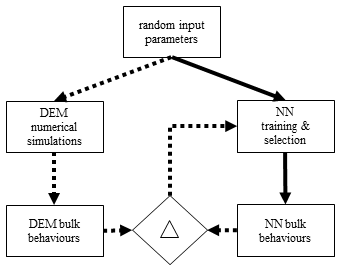
\includegraphics[width=.50\columnwidth]{images/127anntraining}
\caption[ANN training]{ANN training.}
\label{fig:127anntraining}
\end{figure}

Initially, as shown in Fig. \ref{fig:019methodology} in the training phase
(dashed lines) \acs{DEM} simulations are performed
with random initial input parameters.
The behaviours obtained are used to train the following regression models:
\begin{itemize}
  \item{Bayesian linear,}
  \item{Gaussian non linear,}
  \item{Artificial Neural Network (\acs{ANN}).}
\end{itemize}
For all the three models training consists in a loop that continues until the
difference between the outputs of each model and its samples is below the
limit ($\Delta$) (see Chapter \ref{cap:ann} for more details).\\
Thus, we were able to use the \acs{DEM} parameter combinations and their
corresponding bulk values to train the models.
Especially, we divided the samples in three pools: the first, with 70\% of the
samples, as \textit{training set}, the second, with 15\% of the samples, as
\textit{generalization set}, for early stopping, and the third, as \textit{test
set}, as suggested by Haykin (2009). The assignment of each sample to each pool
was random.

\subsection{ANN training concept specifications}
\label{subsec:anntrainingconceptspecifications}

The training of an \acs{ANN} consists in defining the weights and the biases for
each of its neuron.
We first defined the typology of Artificial Neural Networks (\acs{ANNs}) we used and
the input we fed them, see Benvenuti et al. \cite{RefWorks:180}.
Our \acs{ANNs} have three different layers: the input layer has a number of neurons
equal to the number of different inputs of the network, see Fig.
\ref{fig:018nnscheme}, with the scheme of how the Multilayer Perceptron \acs{ANN} ($MLPNN$) derives one
bulk-behaviour-dependent variable from the mutually independent simulation variables.
The hidden (or central) layer's number of neurons was to be investigated. 
The output layer contains one neuron for the output.
The transfer function for the neurons of the central layer is the tangential
sigmoid, while the neuron of the output layer use the linear transfer
function.\\
\begin{figure}[!htb]
\centering
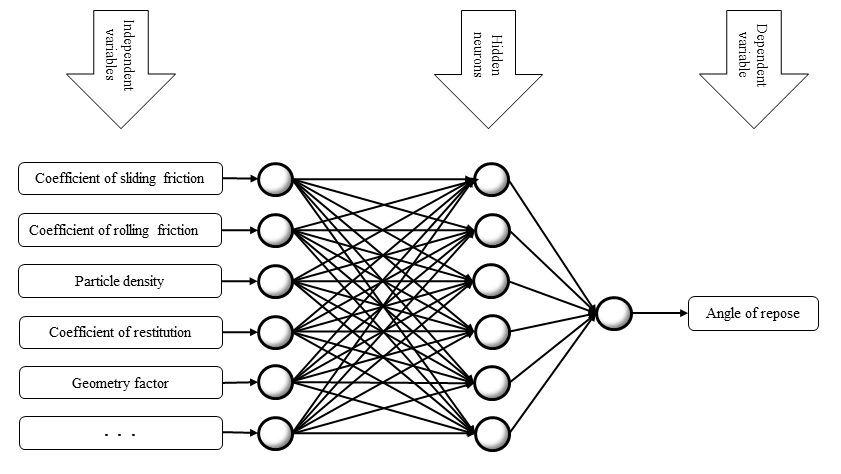
\includegraphics[width=.96\columnwidth]{images/129NN22}
\caption[ANN Scheme]{Artificial Neural Network (\acs{ANN}) Scheme. Regressors
are show in the left-hand side of the image. An example of a response is shown
in the right-hand side of the image.}
\label{fig:018nnscheme}
\end{figure}
We started with all the \acs{DEM} parameter combinations and their corresponding
numerical \acs{mupsh} from the \textit{training set} to create 36 \acs{ANNs} that
differed in their numbers of neurons in the hidden layer (between five to forty neurons).
The \textit{generalization set} was used to speed the training. 
We then determined the coefficient of determination (\acs{r2}), 
\begin{equation}
R^2 = \frac {SSR}{SST} = 1 - \frac {SSE}{SST} .
 \label{eq:rsquare}
\end{equation}

between the
$bulk-macro$ behaviours in the output of the \acs{ANN} and the \textit{test
set} simulations, which were not correlated with the remaining 70\% used for the
training.
Thus, we could select for \acs{mupsh} the \acs{ANN} with the maximum \acs{r2}, 
again as suggested by Vaferi et al. \cite{RefWorks:150}, and we noted its number
of neurons.
We repeated the same \acs{ANN} creation steps for \acs{mush}, \acs{rhob}
and \acs{AoR}, obtaining one trained \acs{ANN} for each bulk value. \\

\subsection{Sinter fine ANN training}
\label{subsec:sinterfineanntraining}

As said, we started with the sinter fine.
The first bulk value \acs{ANN} trained was the \acs{mupsh}, where we achieved a
$\acs{r2} = 0.96$ for an \acs{ANN} with fifteen neurons, a consistent agreement between the 
\acs{DEM} and the \acs{ANN} values, which demonstrates the accurate predictive power of
the \acs{ANN}, compared to the other two methods.
Increasing the number of neurons did not improve the \acs{r2}; it even started to
oscillate with higher numbers of neurons.
We subsequently obtained the optimal number of neurons for all \acs{ANNs}.\\
Later, we obtained Fig.
\ref{fig:022regression}, where the corresponding plot for the \acs{ANN} with the maximum \acs{r2} is shown. 
Each circle represents one of the 546 simulations.
\begin{figure}[!h] 
\centering 
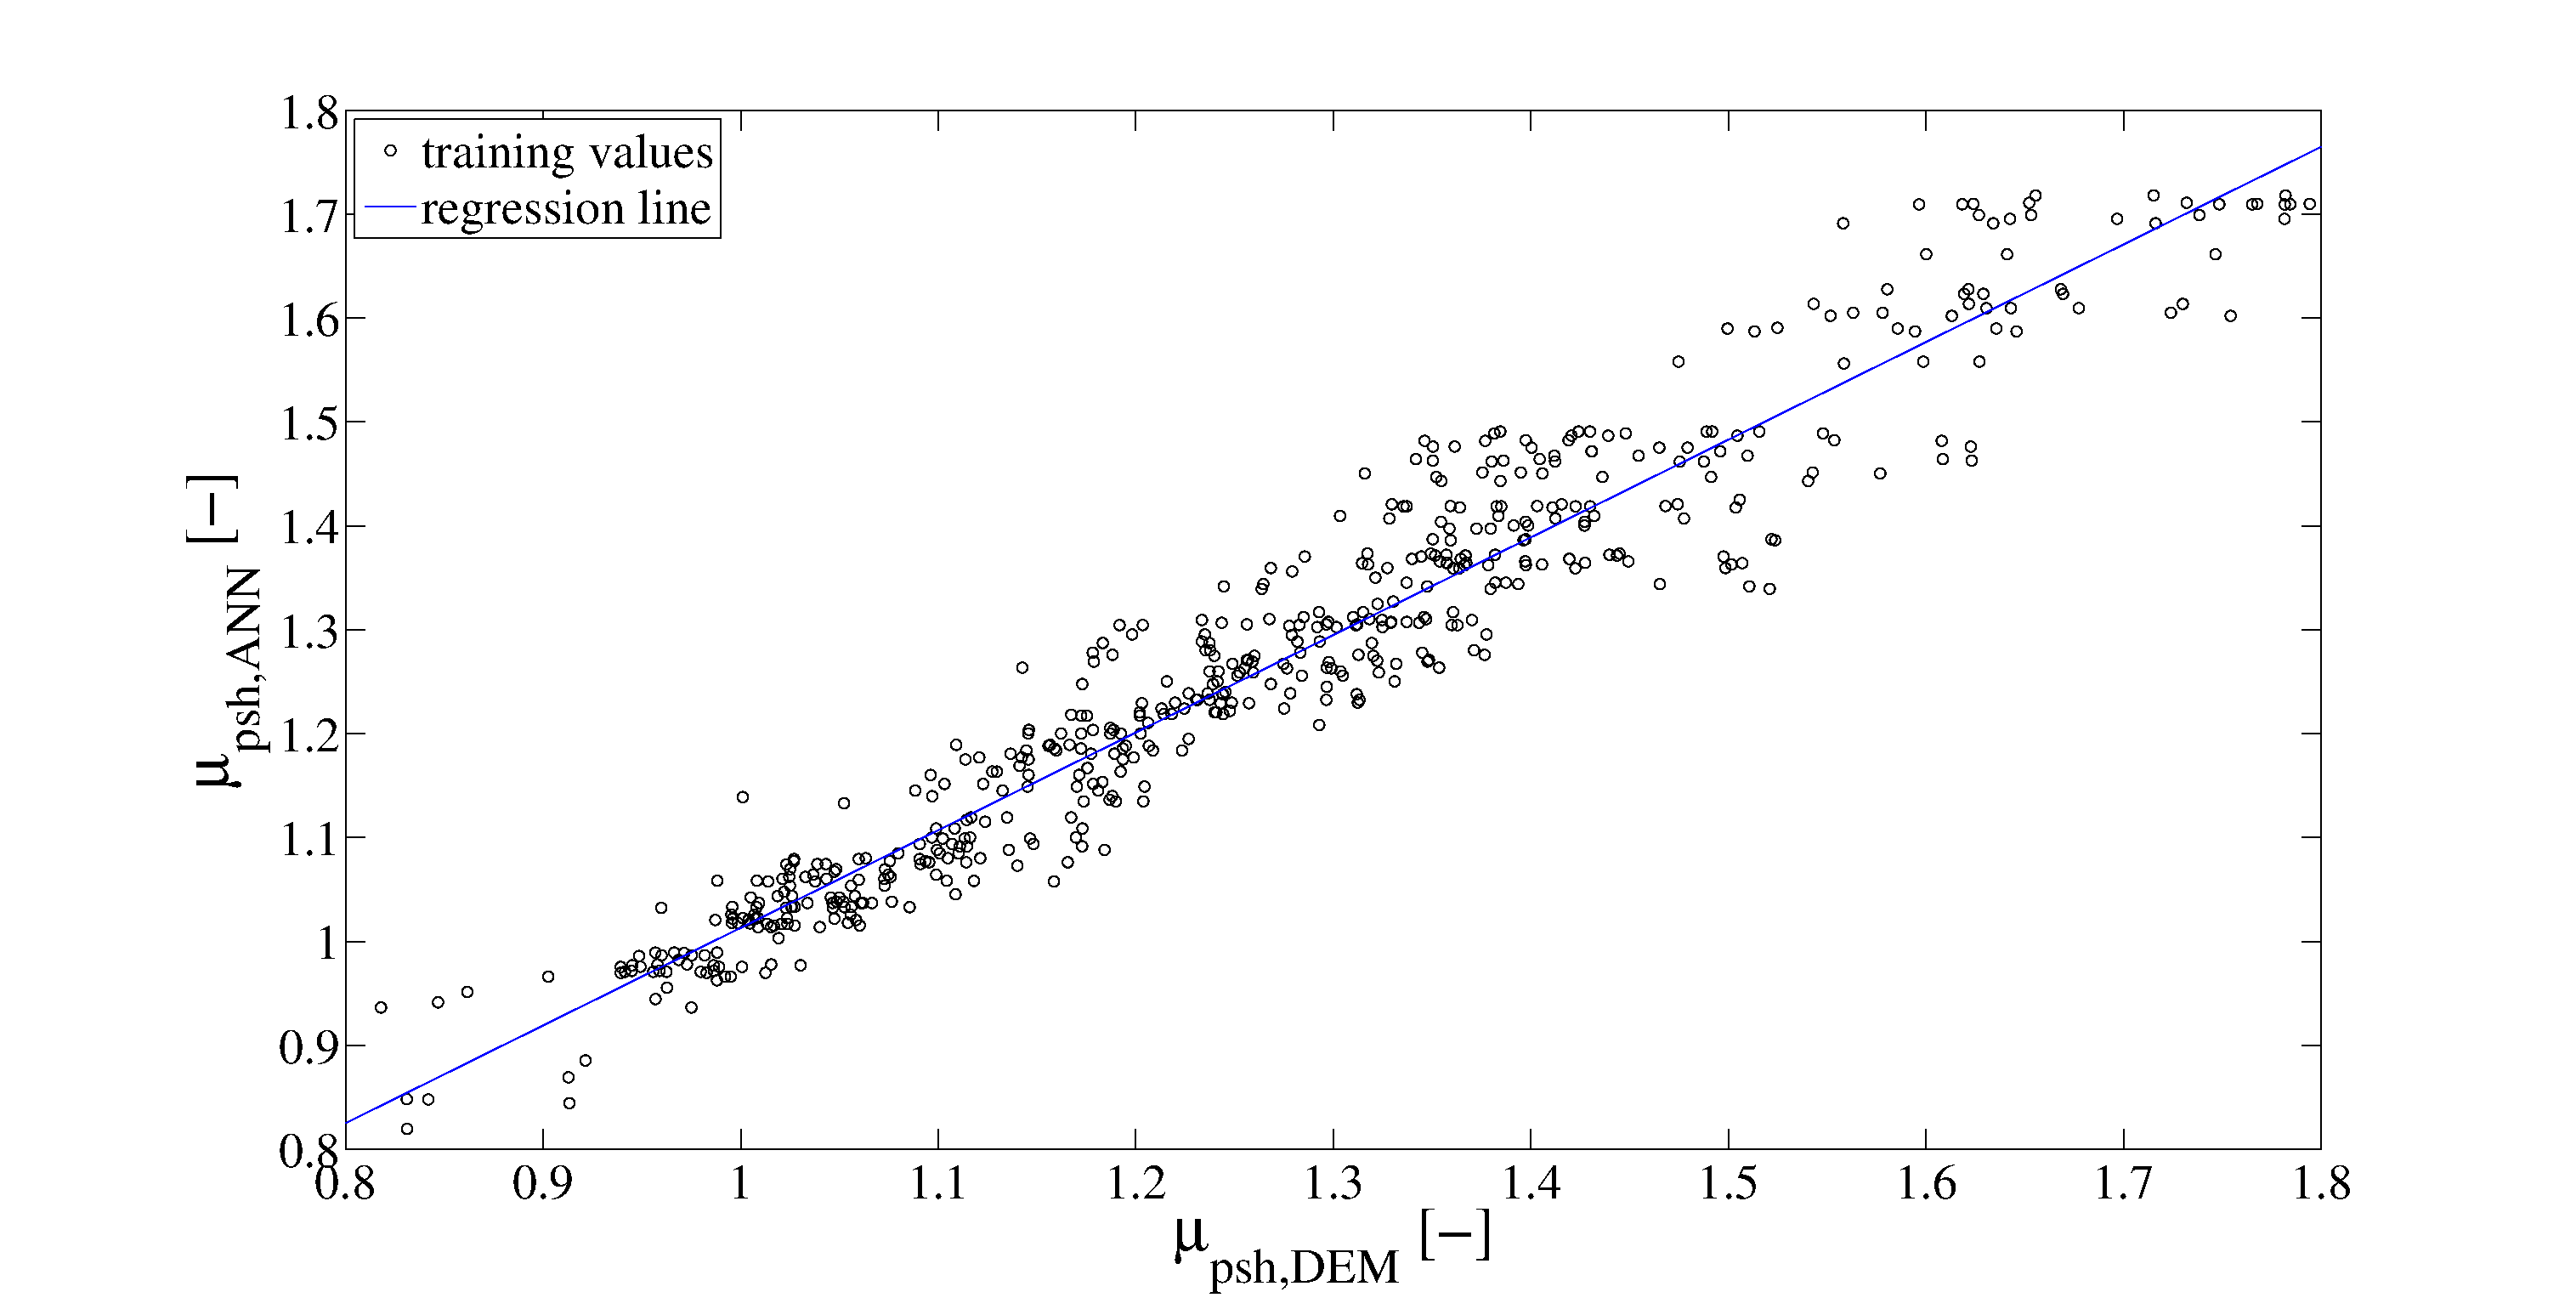
\includegraphics[width=.80\columnwidth]{images/022regression.eps}
%[width=.96\textwidth]
\caption[Comparison between prediction of the trained ANN and full DEM
simulation]{Comparison between prediction of the trained Artificial Neural
Network (\acs{ANN}) and 546 
\wrong{write down all the simulations performed at the end.}
full DEM simulations of the coefficient of pre-shear
(\acs{mupsh}).}
\label{fig:022regression} 
\end{figure}

\section{Statistical tools comparison}
\label{sec:statisticaltoolscomparison}

%\begin{figure}[htbp]
  %\null\hfill
  \subfloat[SCT Bayesian linear regressor.]{
	  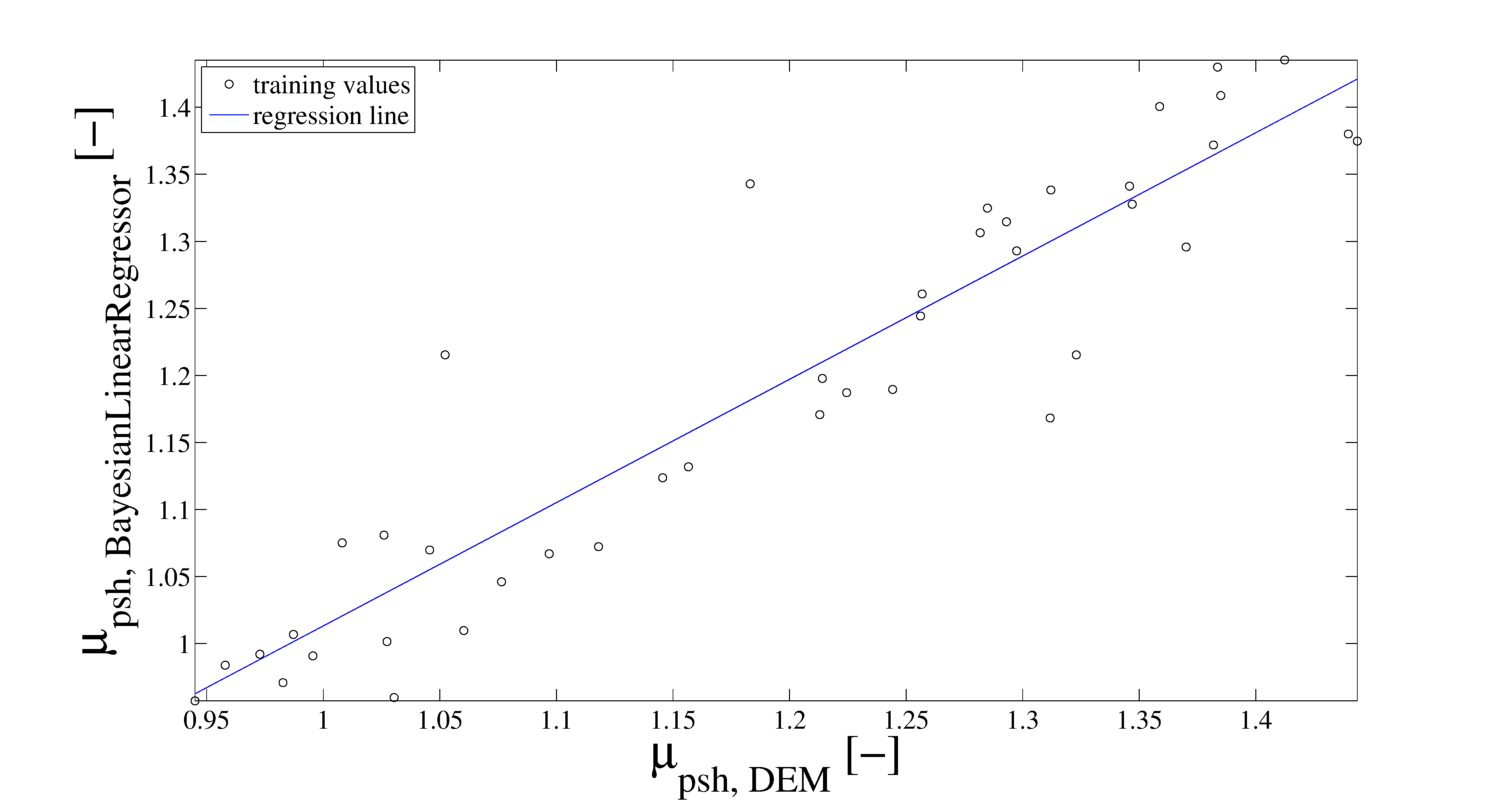
\includegraphics[width=.48\columnwidth]{images/069sctbayesianlinearregressor}
	  \label{fig:069sctbayesianlinearregressor}
  }
  \quad
    \subfloat[SCT Gaussian non linear regressor.]{
	  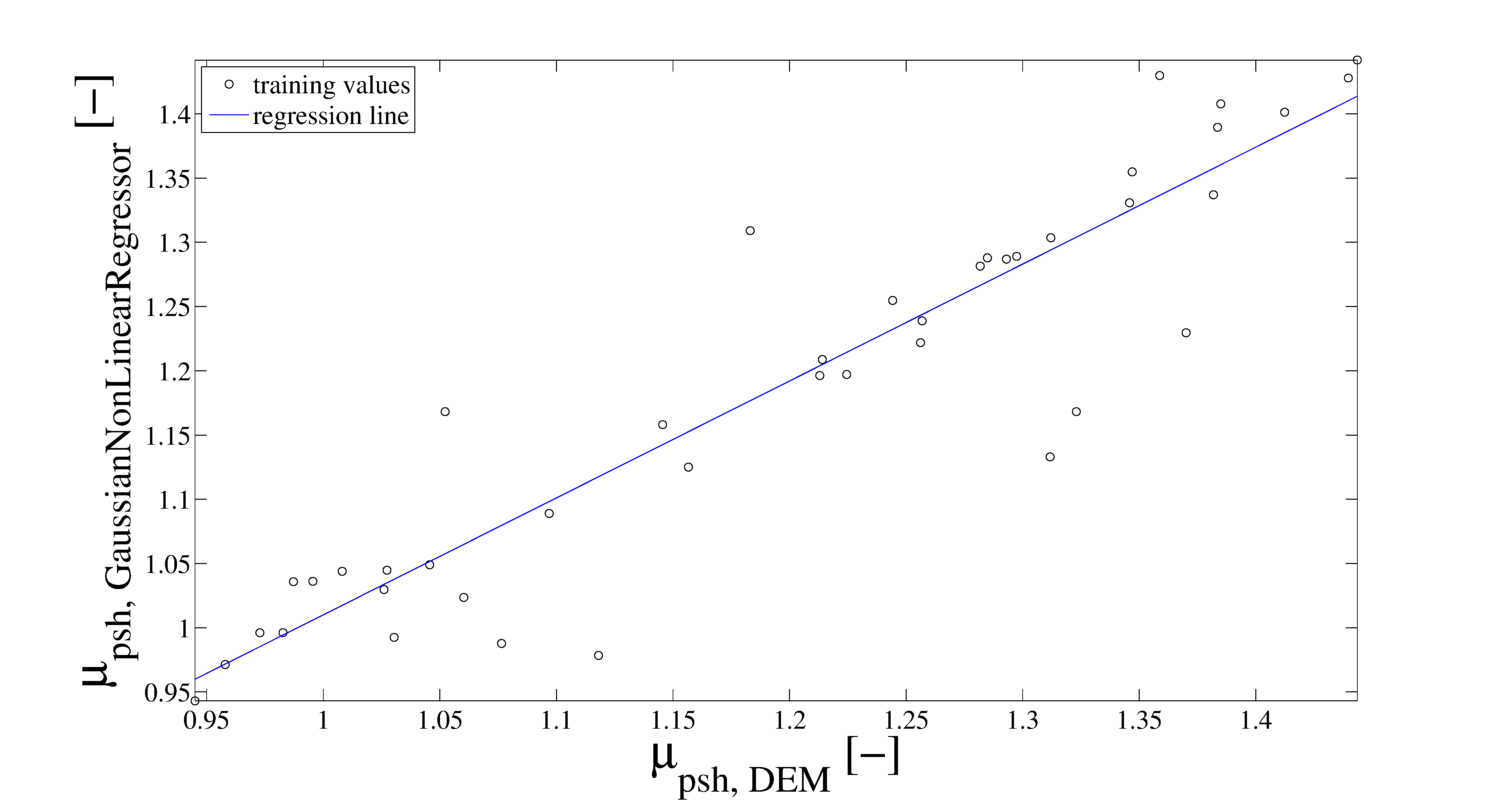
\includegraphics[width=.48\columnwidth]{images/070sctgaussiannonlinearregressor}
	  \label{fig:070sctgaussiannonlinearregressor}
  }
  \\
 % \hfill
  \subfloat[SCT ANN non linear regression.]{
	  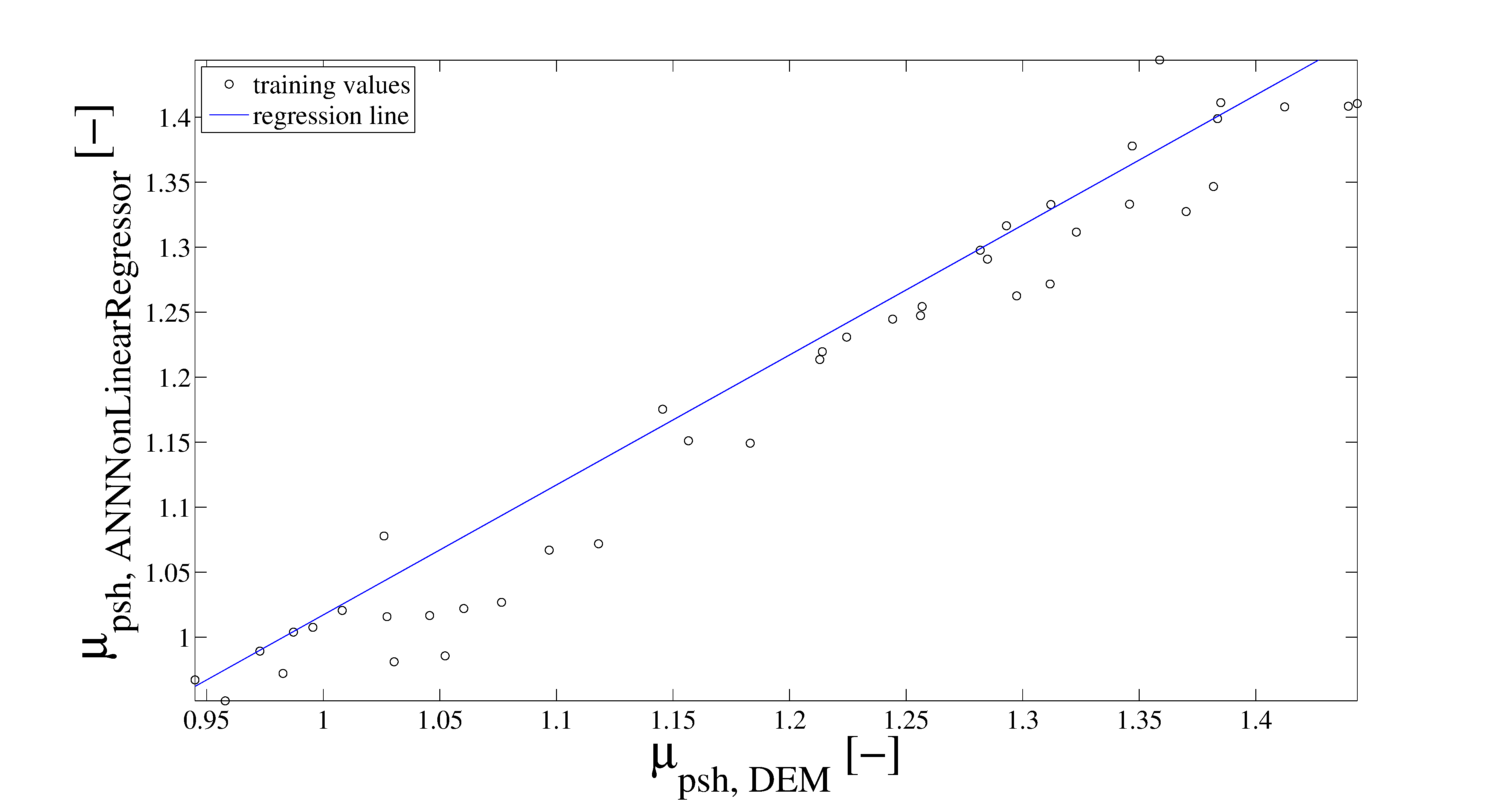
\includegraphics[width=.48\columnwidth]{images/071annnonlinearregressor}
	  \label{fig:071annnonlinearregressor}
  }
  \quad
    \subfloat[AoR Bayesian linear regressor.]{
	  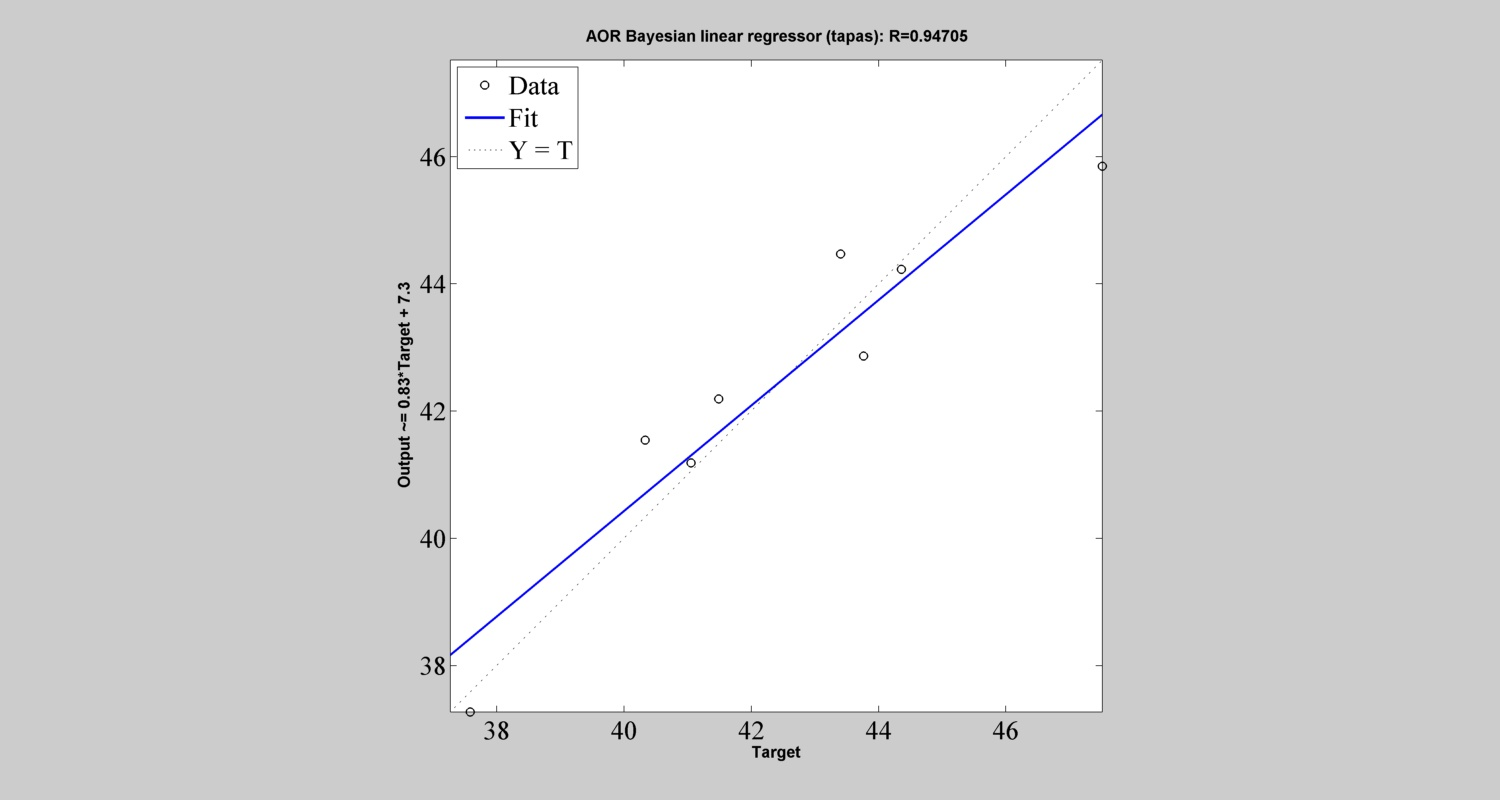
\includegraphics[width=.48\columnwidth]{images/072aorbayesianlinearregression}
	  \label{fig:072aorbayesianlinearregression}  }
  \\
    \subfloat[AoR Gaussian non linear regressor.]{
	  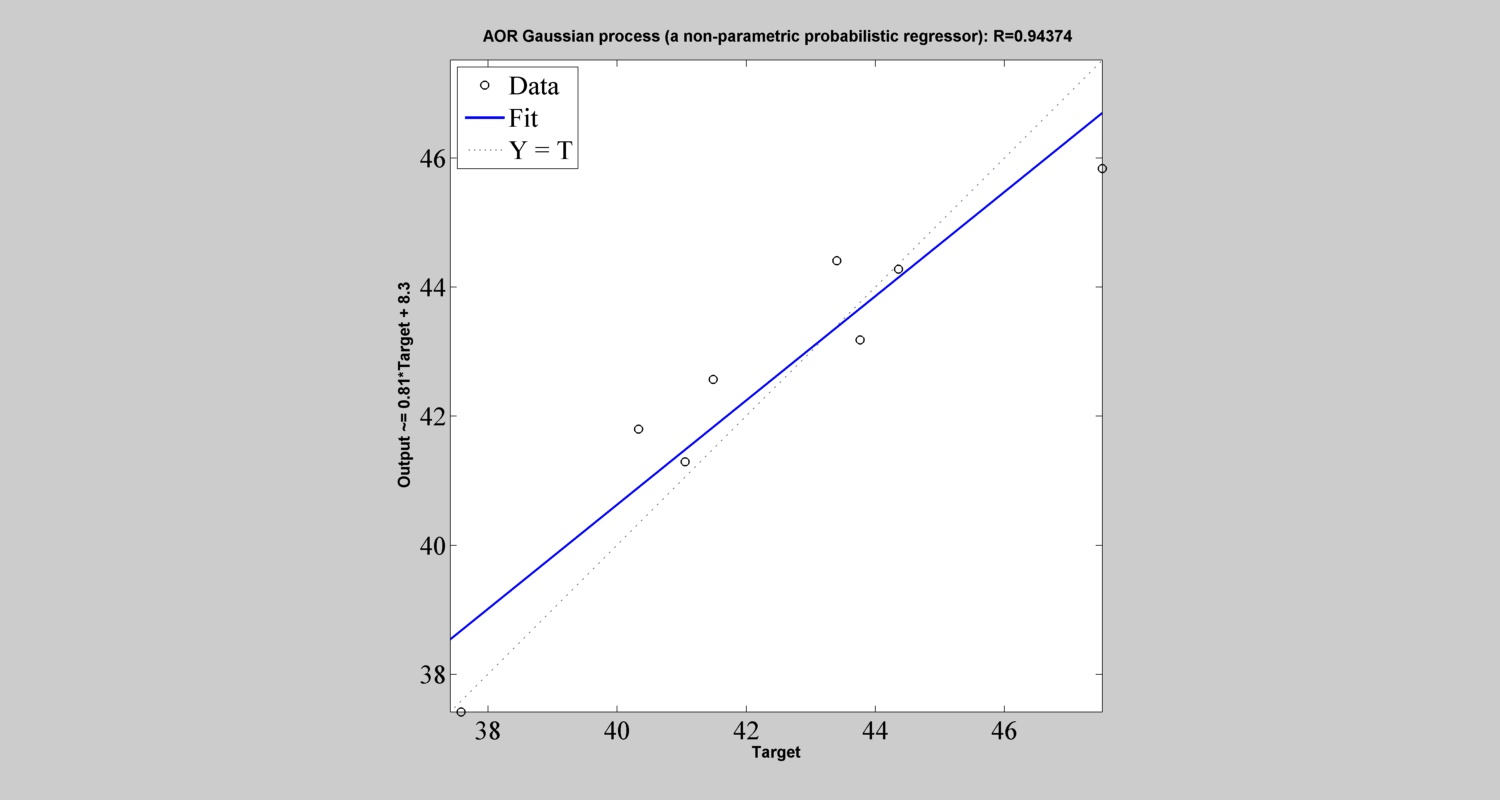
\includegraphics[width=.48\columnwidth]{images/073aorgaussiannonlinearregression}
	  \label{fig:073aorgaussiannonlinearregression}
  }
  \quad
 % \hfill
  \subfloat[AoR ANN non linear regression.]{
	  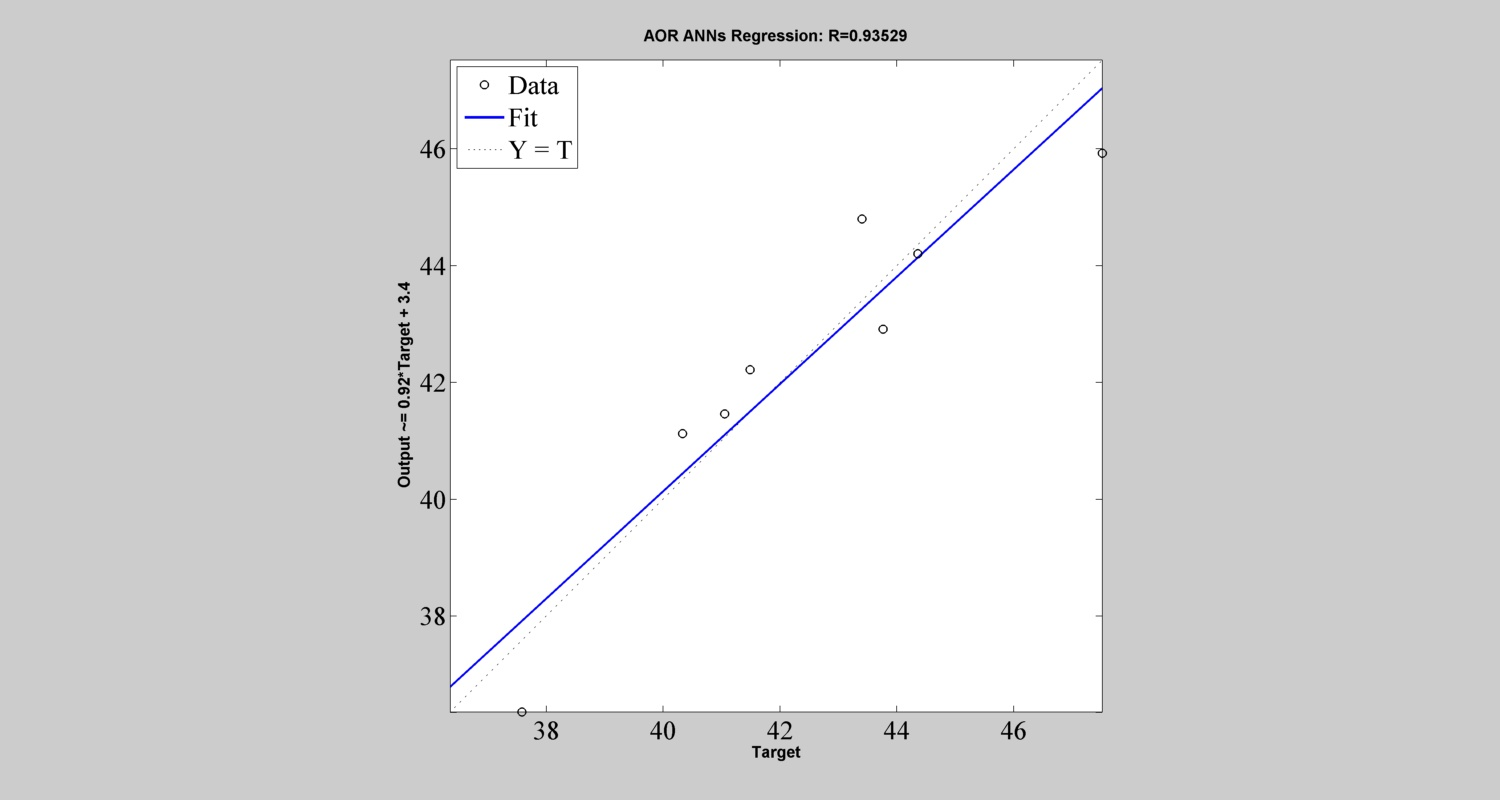
\includegraphics[width=.48\columnwidth]{images/074aorannnonlinearegression}
	  \label{fig:074aorannnonlinearegression}
  }
 % \hfill\null
  \caption{Regressions.}
  \label{fig:077regressions}
\end{figure}

% \begin{figure}%[!h] 
% \centering 
% 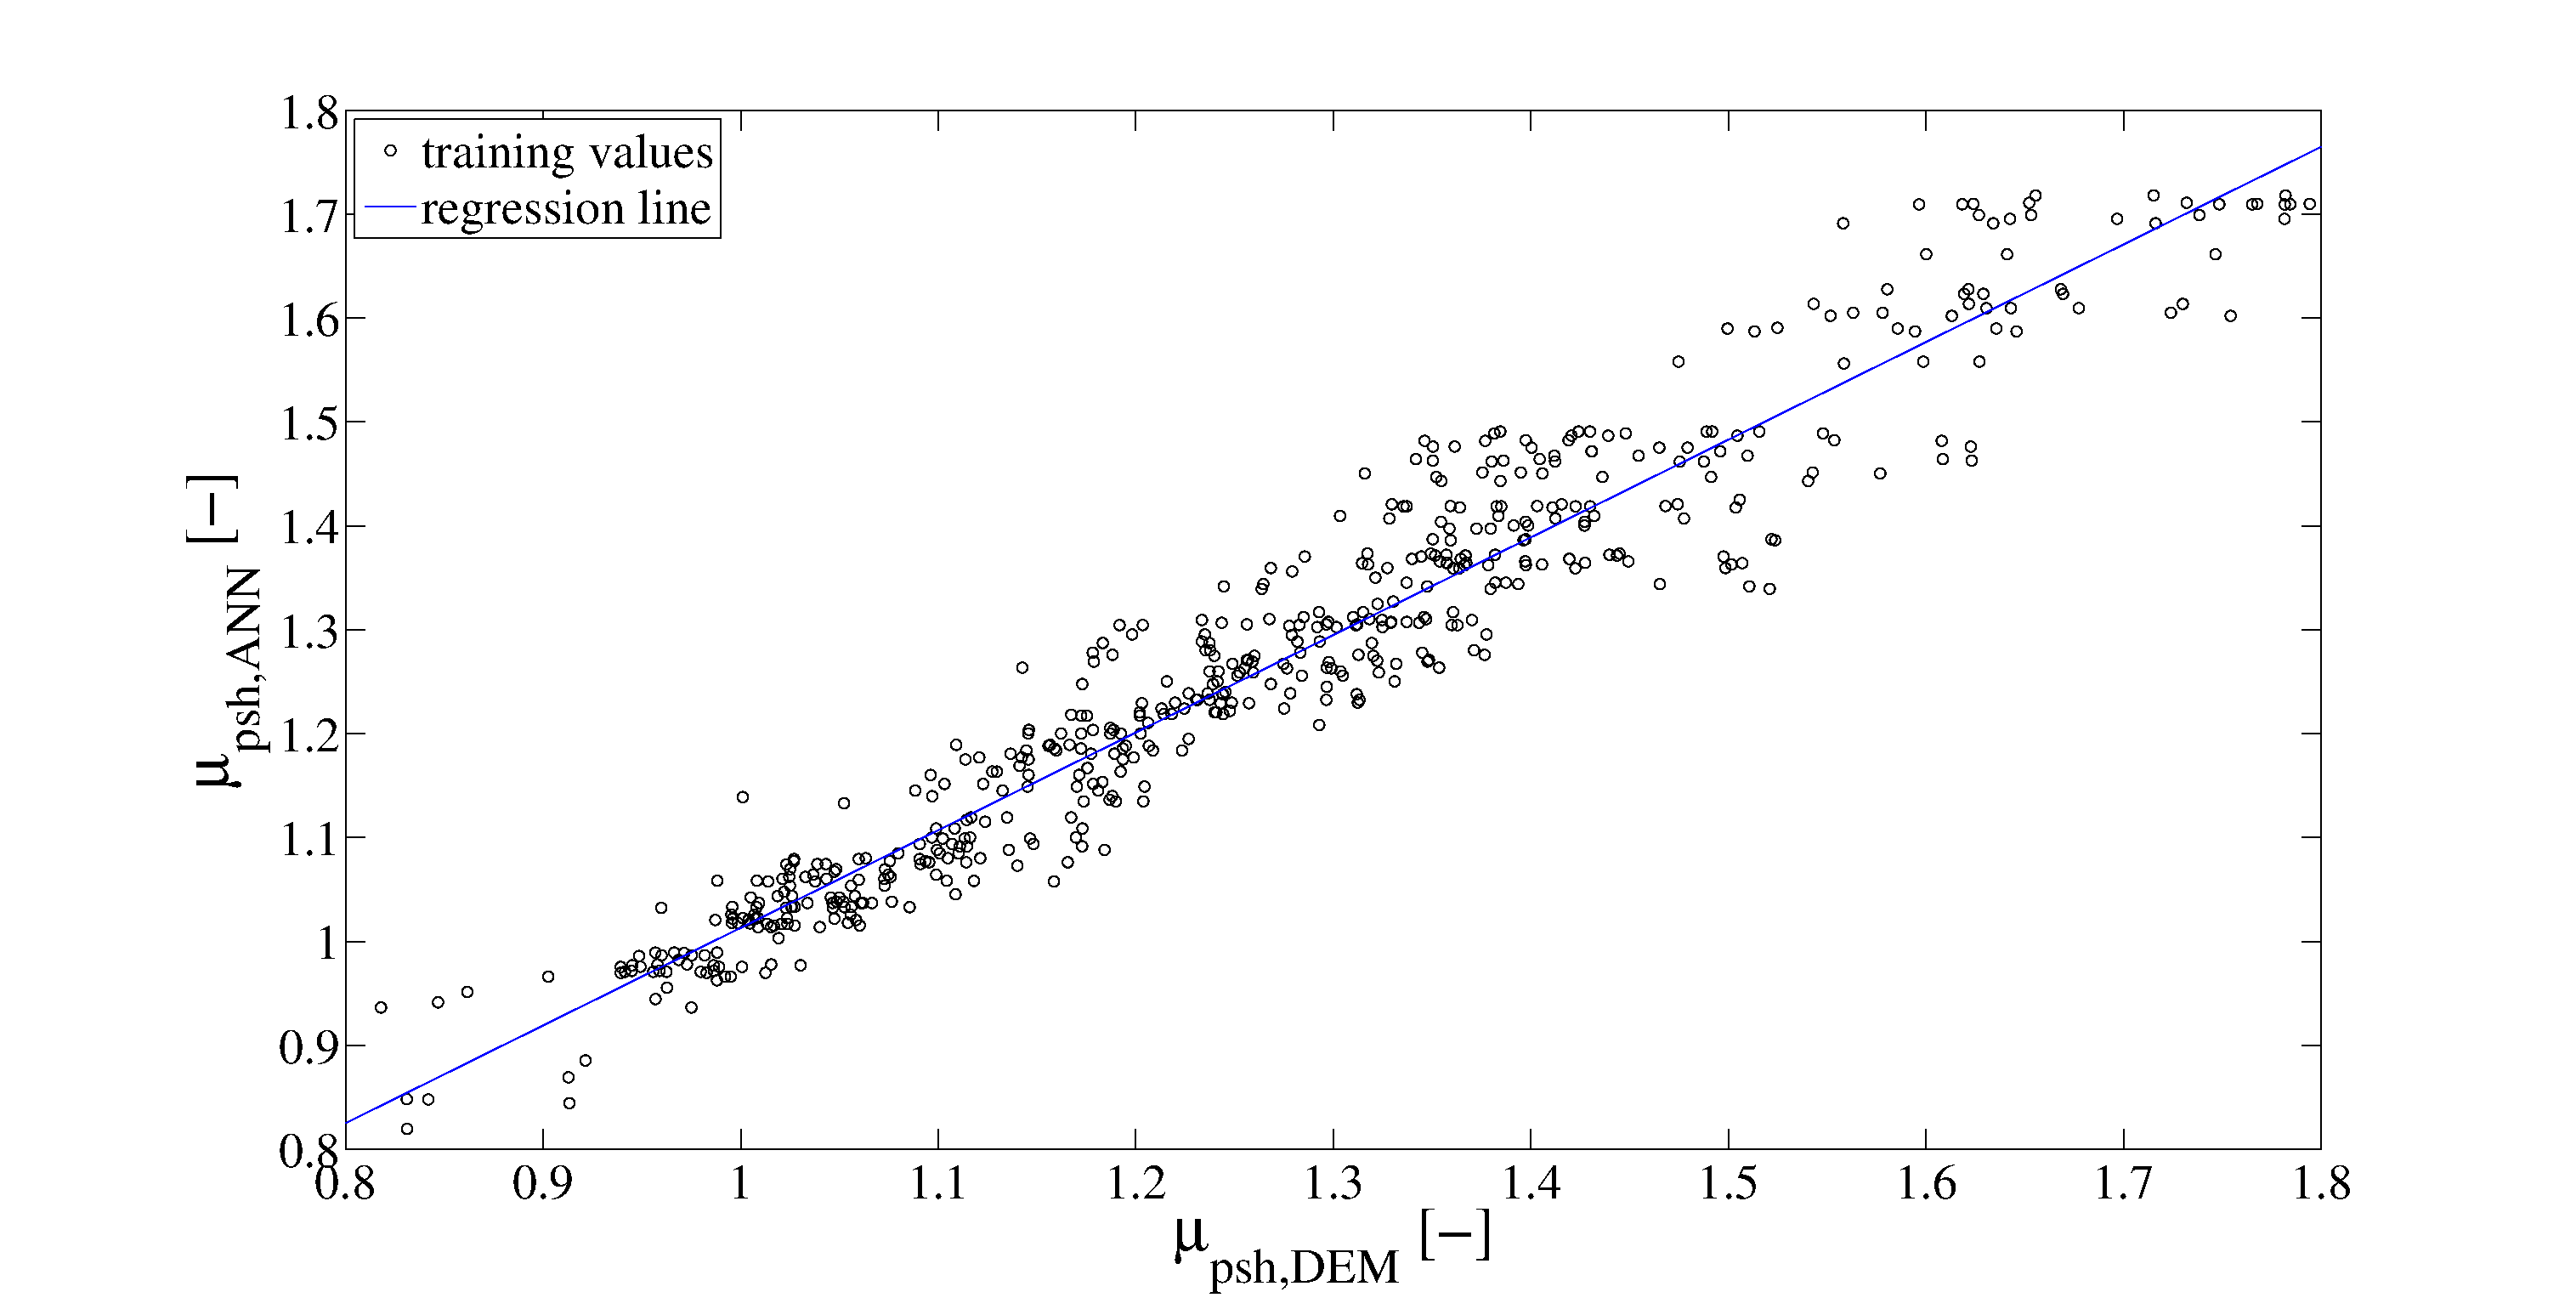
\includegraphics[width=.80\columnwidth]{images/022regression.eps}
% %[width=.48\textwidth]
% \caption[Comparison between prediction of the trained ANN and full DEM
% simulation]{Comparison between prediction of the trained Artificial Neural
% Network ($ANN$) and 546 
% \wrong{write down all the simulations performed at the end.}
% full DEM simulations of the coefficient of pre-shear
% (\ac{mupsh}).}
% \label{fig:022regression} 
% \end{figure}
\begin{figure}[htbp]
	\centering
  %\null\hfill
  \subfloat[SCT Bayesian linear regressor.]{
	  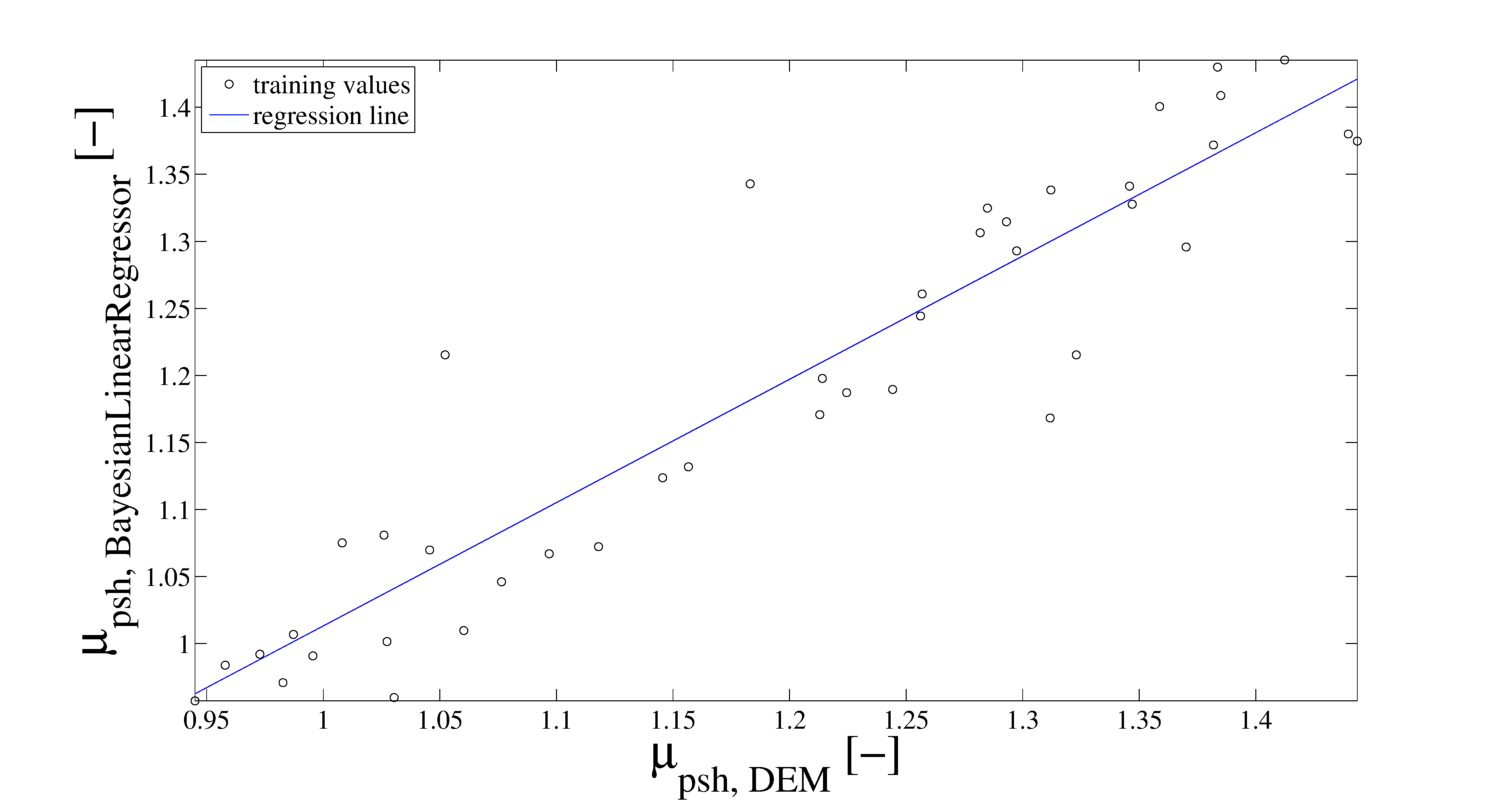
\includegraphics[width=.75\columnwidth]{images/137SCTBayesianLinearRegressor}
	  \label{fig:137SCTBayesianLinearRegressor}
  }
  \\
    \subfloat[SCT Gaussian non linear regressor.]{
	  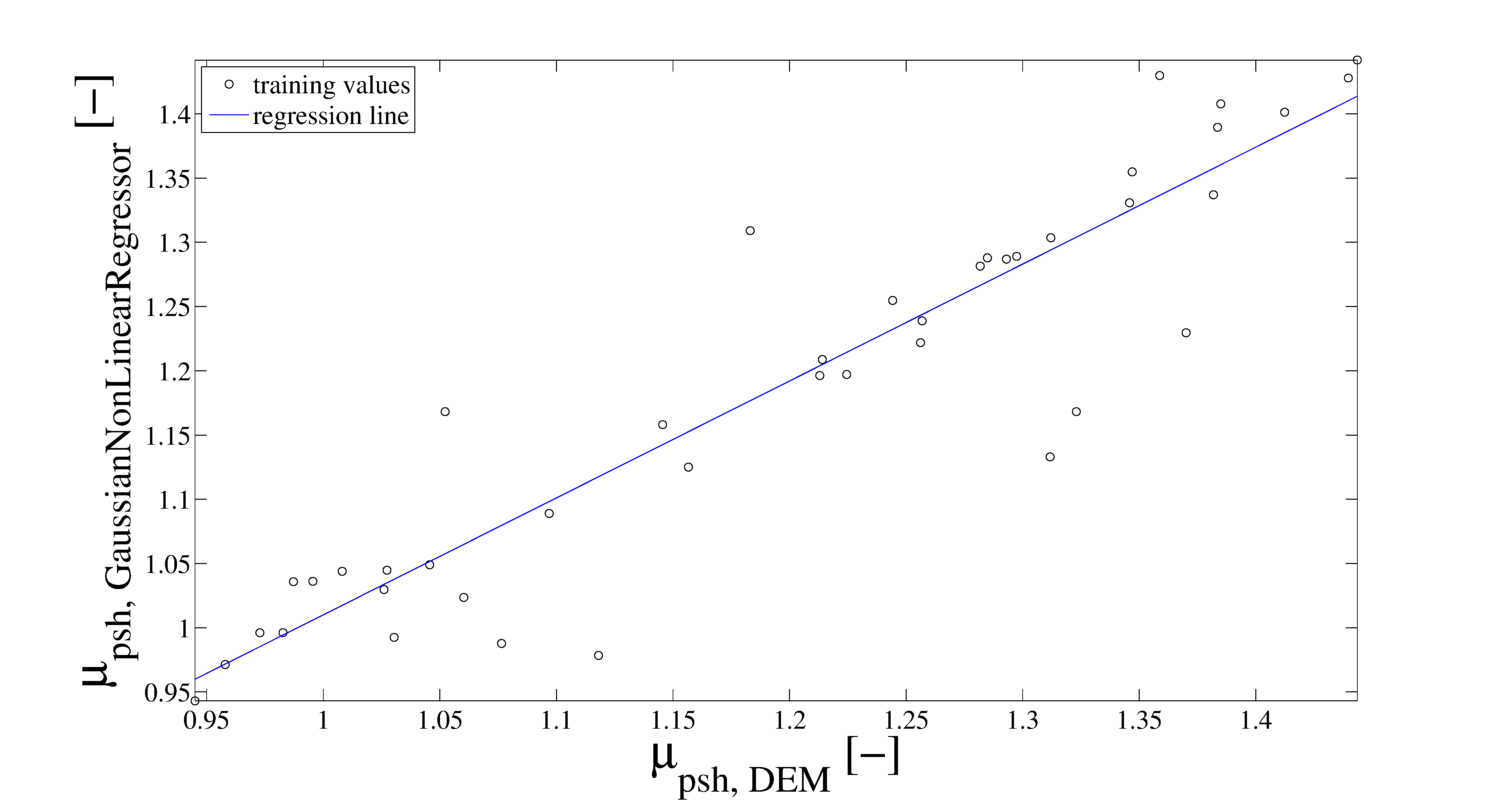
\includegraphics[width=.75\columnwidth]{images/138SCTGaussianNonLinearRegressor}
	  \label{fig:138SCTGaussianNonLinearRegressor}
  }
  \\
 % \hfill
  \subfloat[SCT ANN non linear regression.]{
	  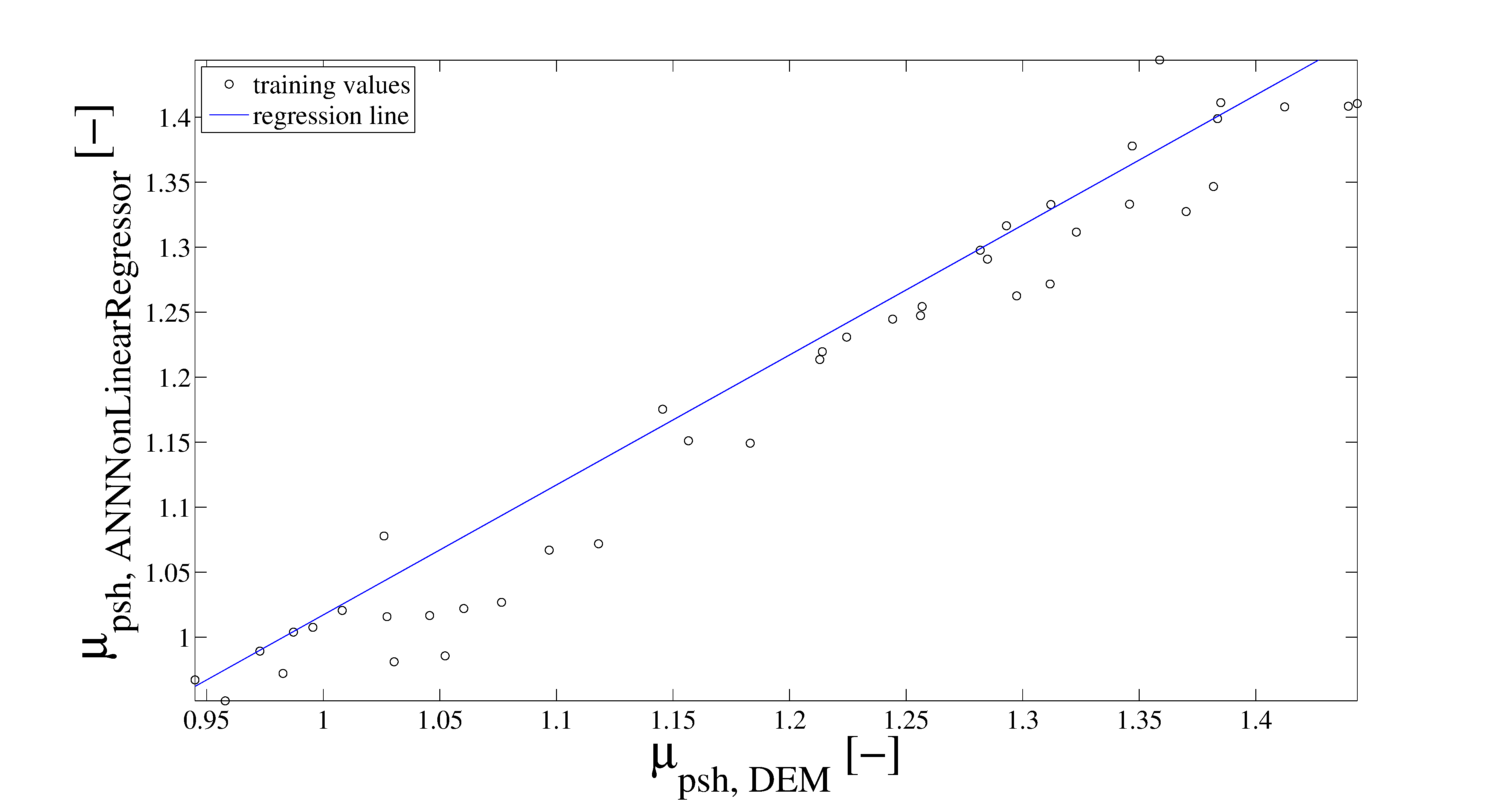
\includegraphics[width=.75\columnwidth]{images/139SCTANNNonLinearRegressor}
	  \label{fig:139SCTANNNonLinearRegressor}
  }
  \caption{Regressions comparison for the \acs{mupsh}.}
  \label{fig:143sctregressions}
\end{figure}

% \begin{figure}%[!h] 
% \centering 
% 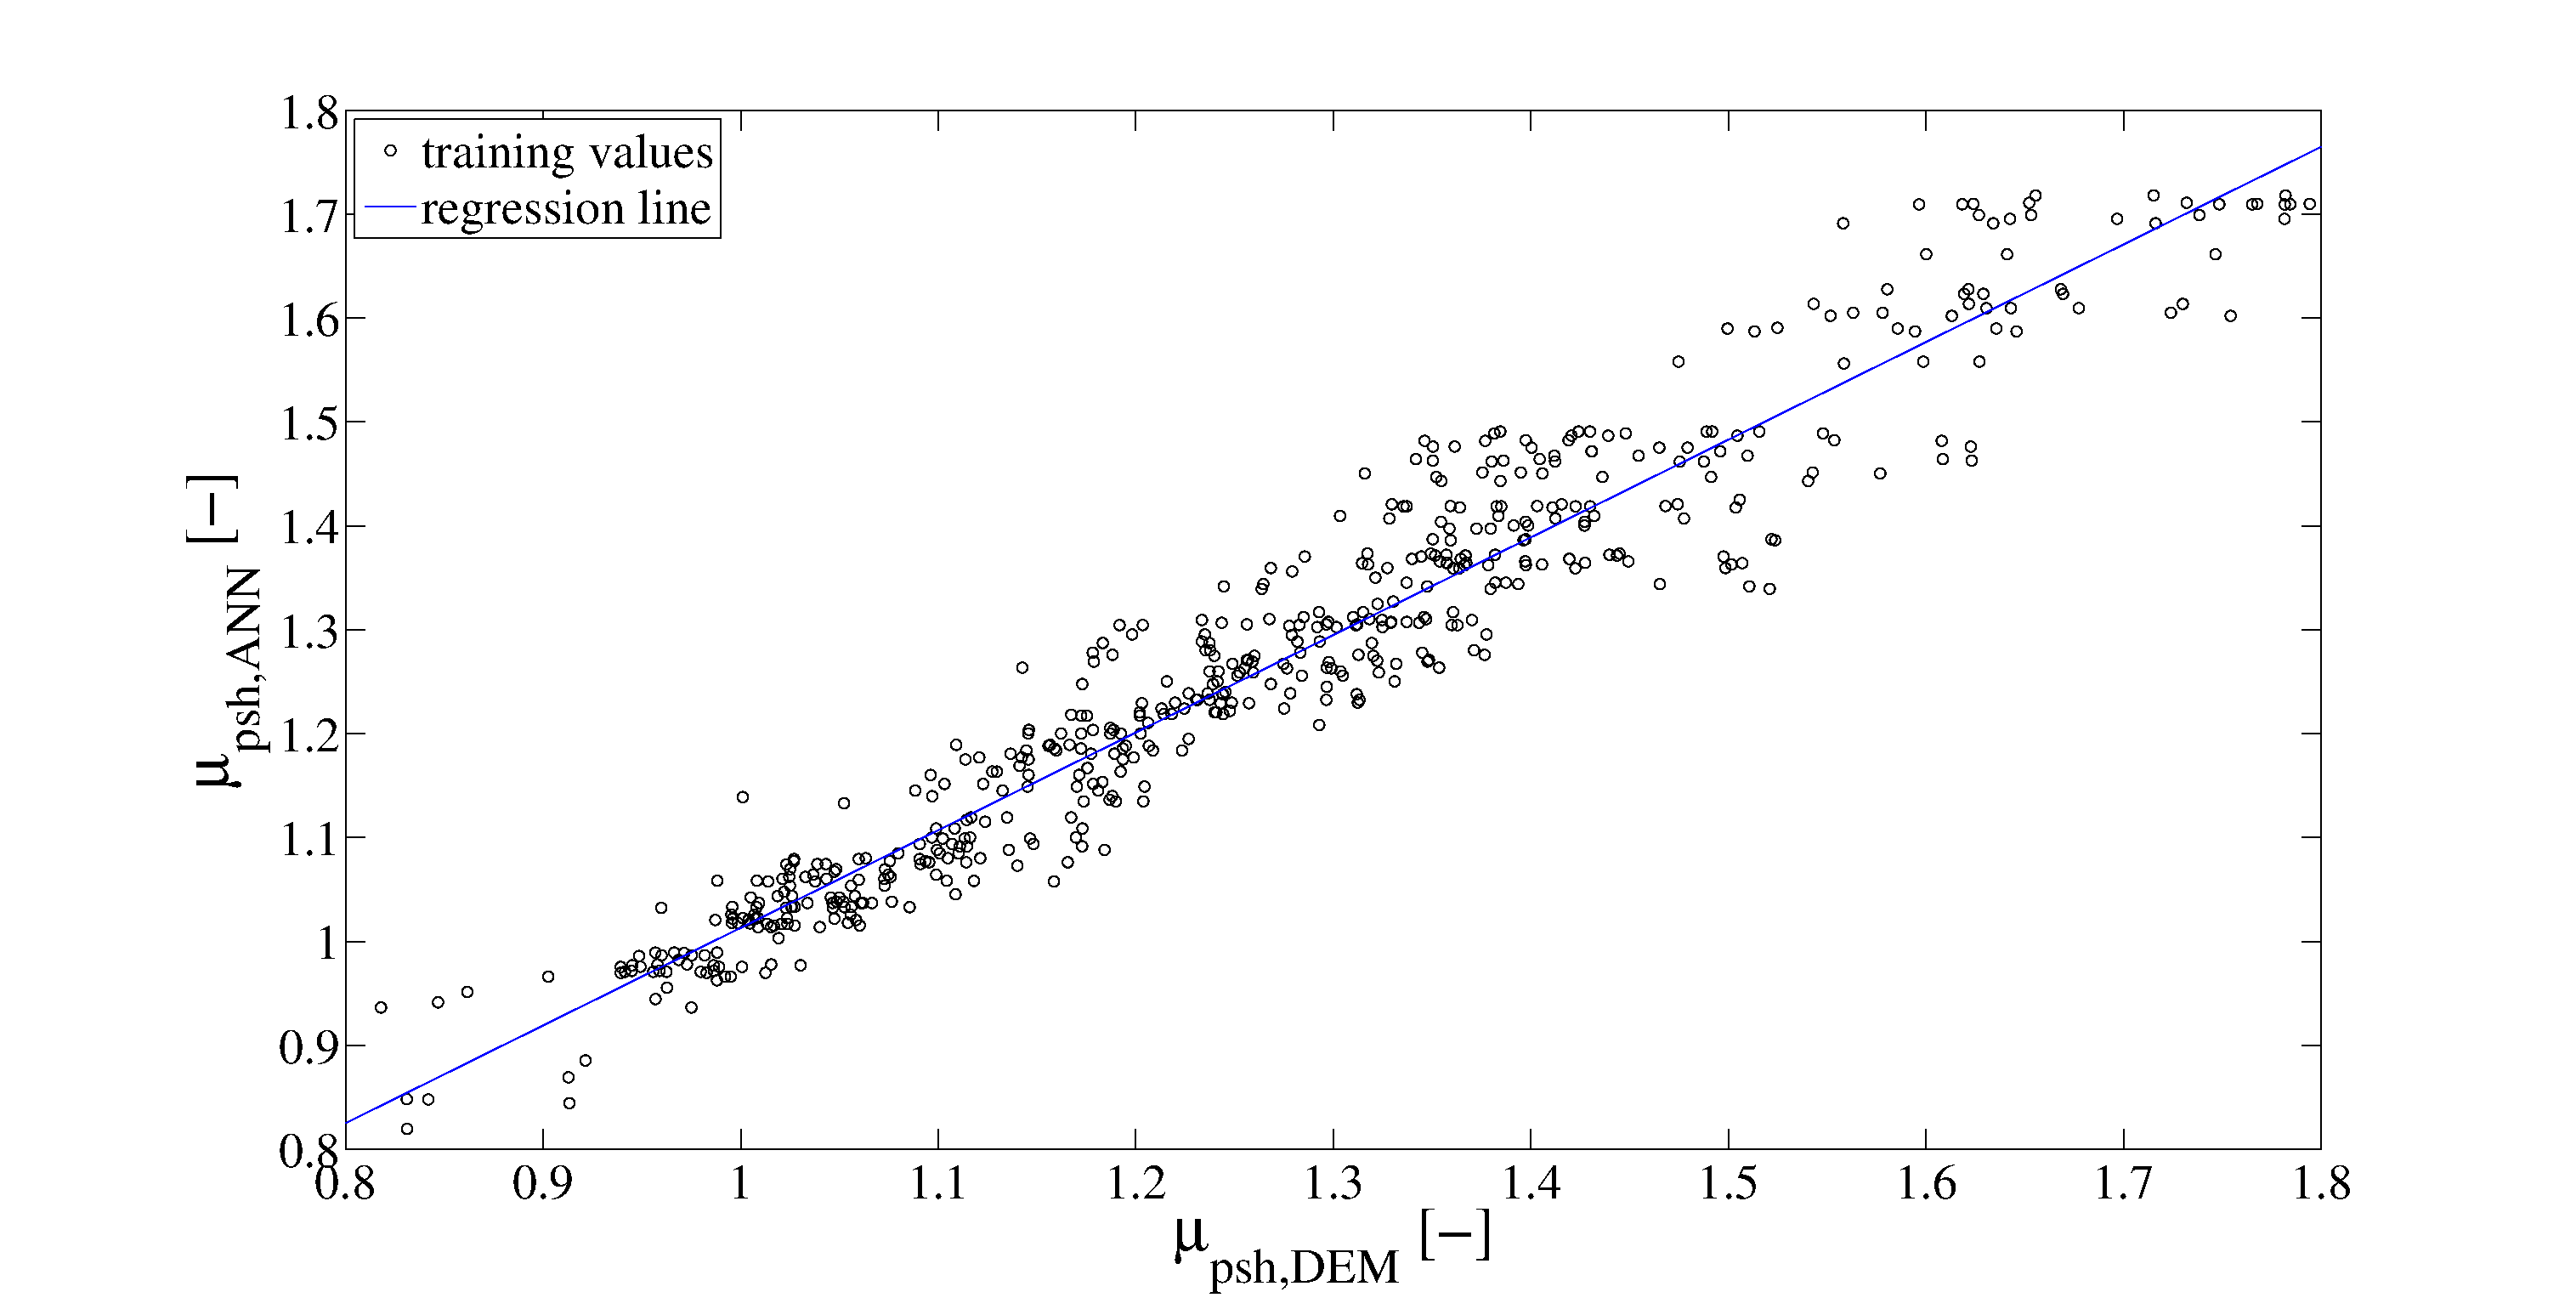
\includegraphics[width=.80\columnwidth]{images/022regression.eps}
% %[width=.48\textwidth]
% \caption[Comparison between prediction of the trained ANN and full DEM
% simulation]{Comparison between prediction of the trained Artificial Neural
% Network (\acs{ANN}) and 546 
% \wrong{write down all the simulations performed at the end.}
% full DEM simulations of the coefficient of pre-shear
% (\acs{mupsh}).}
% \label{fig:022regression} 
% \end{figure}
\begin{figure}[htbp]
	\centering

	 % \resizebox{12cm}{!}{\input{images/137SCTBayesianLinearRegressor.tikz}}


    \subfloat[AoR Bayesian linear regressor.]{
	  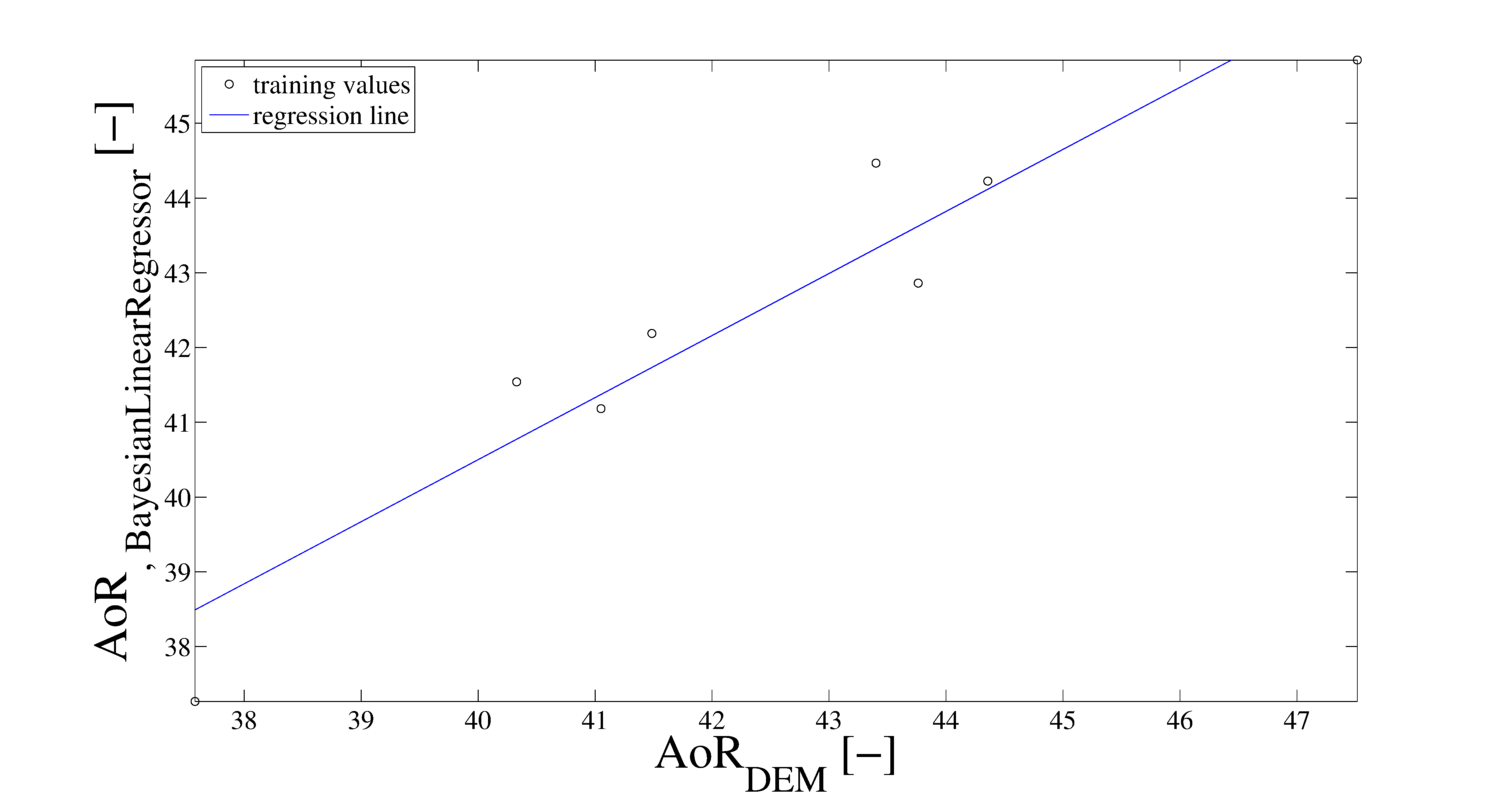
\includegraphics[width=.75\columnwidth]{images/140AoRBayesianLinearRegressor}
	  \label{fig:140AoRBayesianLinearRegressor}  }
  \\
    \subfloat[AoR Gaussian non linear regressor.]{
	  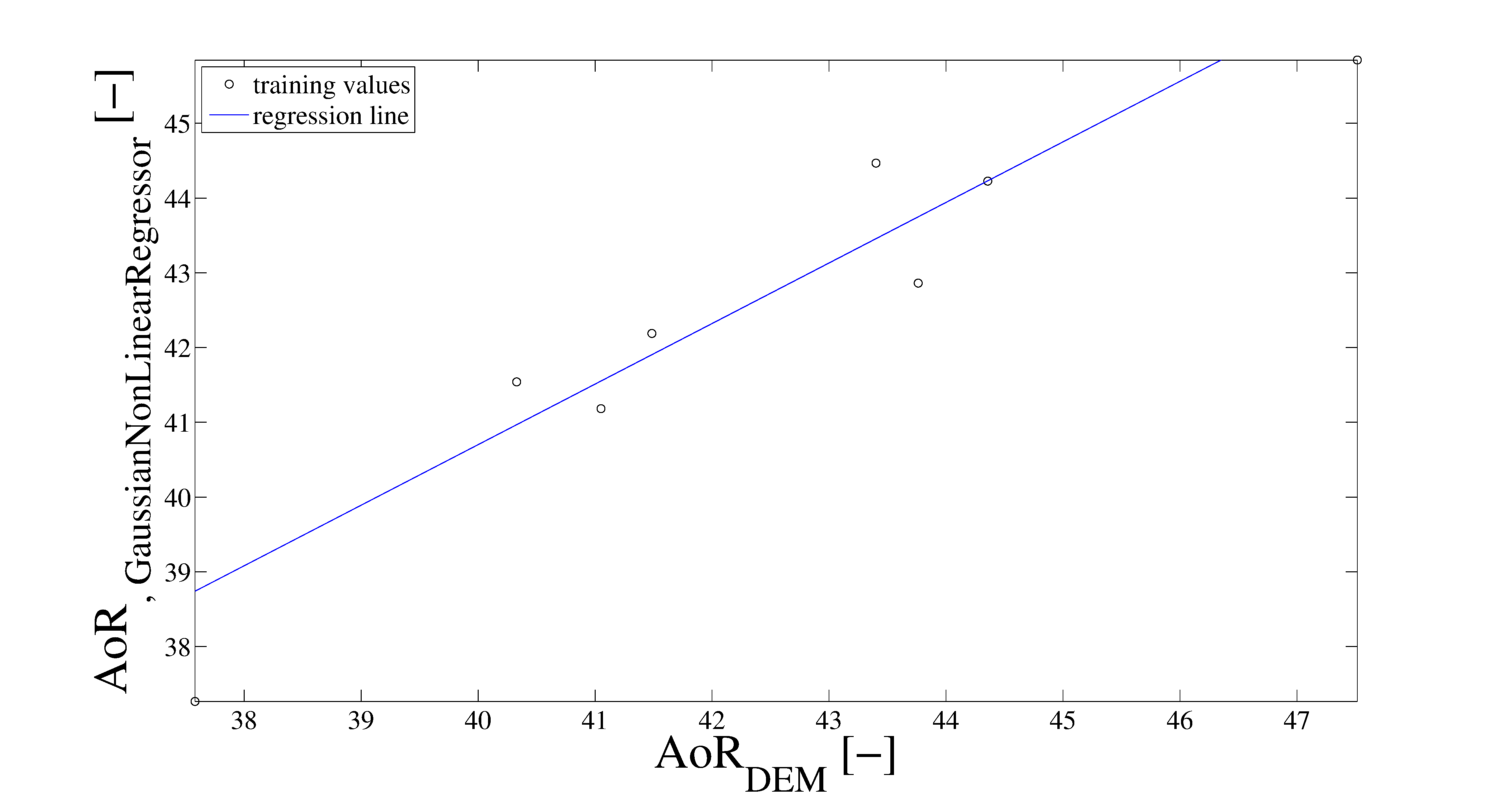
\includegraphics[width=.75\columnwidth]{images/141AoRGaussianNonLinearRegressor}
	  \label{fig:141AoRGaussianNonLinearRegressor}
  }
  \\
 % \hfill
  \subfloat[AoR ANN non linear regression.]{
	  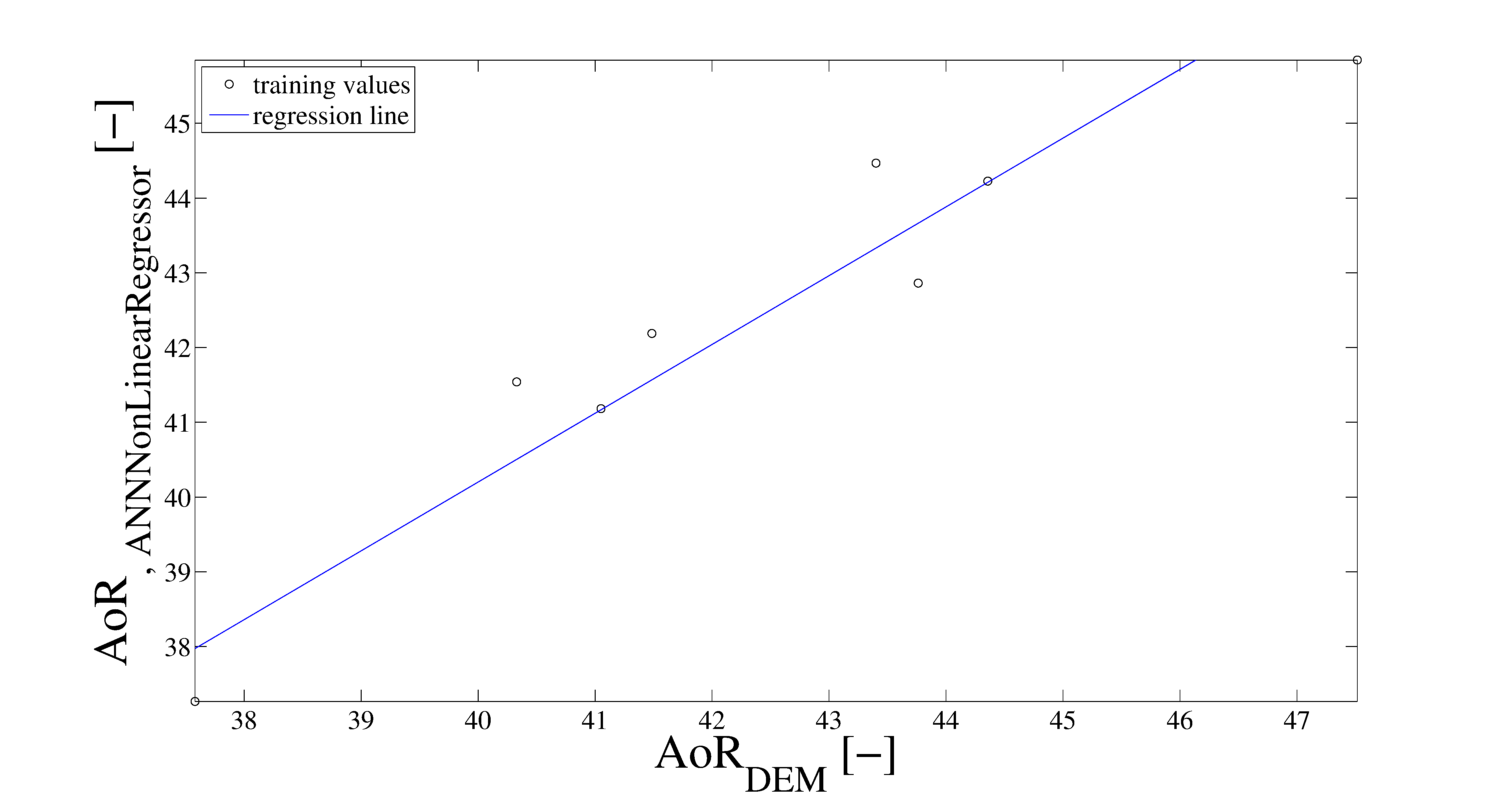
\includegraphics[width=.75\columnwidth]{images/142AoRANNNonLinearRegressor}
	  \label{fig:142AoRANNNonLinearRegressor}
  }
 % \hfill\null
  \caption{Regressions comparison for the \acs{AoR}.}
  \label{fig:144aorregressions}
\end{figure}

% \begin{figure}%[!h] 
% \centering 
% 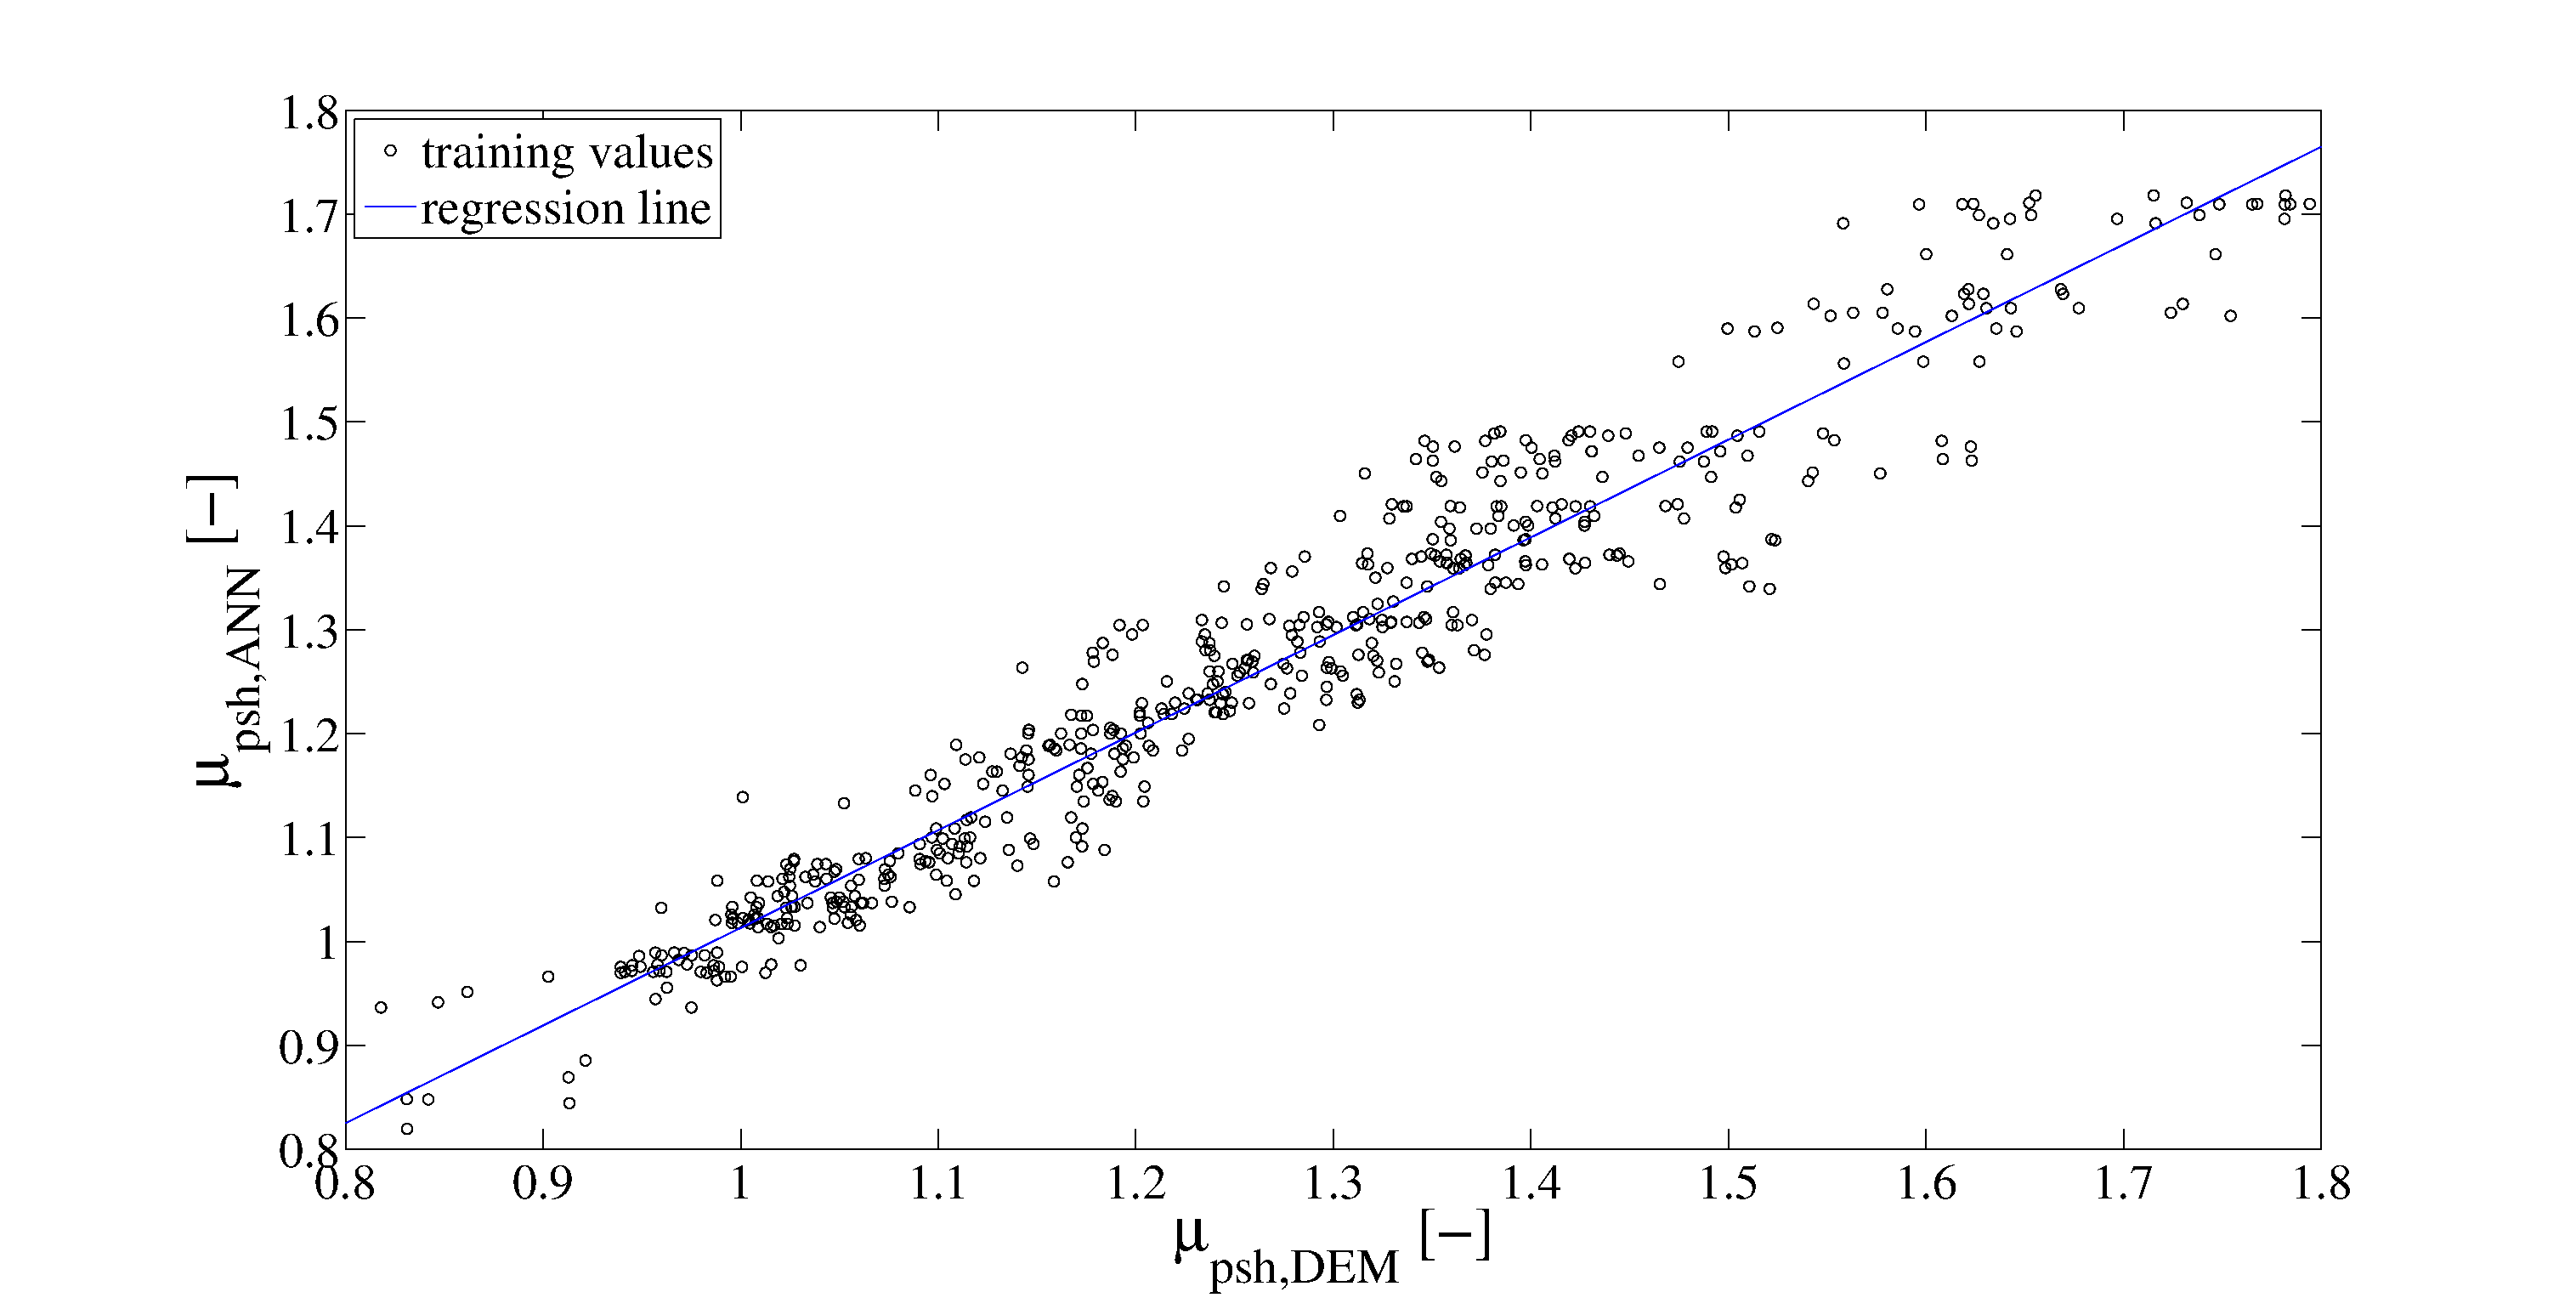
\includegraphics[width=.80\columnwidth]{images/022regression.eps}
% %[width=.48\textwidth]
% \caption[Comparison between prediction of the trained ANN and full DEM
% simulation]{Comparison between prediction of the trained Artificial Neural
% Network (\acs{ANN}) and 546 
% \wrong{write down all the simulations performed at the end.}
% full DEM simulations of the coefficient of pre-shear
% (\acs{mupsh}).}
% \label{fig:022regression} 
% \end{figure}

We checked \acs{r2}, \textit{mean absolute error}, 
\begin{equation}
MAE = \frac{\sum _{i=1}^{n} (x_{i}-\widehat{x}_{i})}{n} ,
\label{eq:meanAbsoluteError}
\end{equation}
\textit{mean squared error},
\begin{equation}
MSE = \frac{\sum _{i=1}^{n} (x_{i}-\widehat{x}_{i})^{2}}{n}
\label{eq:meanSquareError}
\end{equation}
and \textit{root mean squared error},
\begin{equation}
RMSE = \sqrt{\frac{\sum _{i=1}^{n} (x_{i}-\widehat{x}_{i})^{2}}{n}}
\label{eq:rootMeanSquareError}
\end{equation}
for the \textit{Bayesian linear
regression}, the \textit{Gaussian nonlinear
regression}, and the
\textit{\acs{ANN} regression} to establish the most effective method.
All were trained with the same training set. 
For instance, a comparison of the \acs{r2} for the \acs{mupsh} can be see in 
Fig. \ref{fig:069sctbayesianlinearregressor},
Fig. \ref{fig:070sctgaussiannonlinearregressor}) Fig.
\ref{fig:071annnonlinearregressor}.\\
In fact, the check was performed for each method by comparing the \acs{DEM} bulk
values of the test set against the bulk values predicted by each method from the 
corresponding \acs{DEM} input values of the test set. \\
Table \ref{tab:15regressionvalues} shows a quantitative comparison between the
three methods. 
\begin{table}[htbp]
  \centering

    \begin{tabular}{lccc}
    \hline
          & Bayesian & Gaussian & ANN \\
          \hline
    Coefficient of determination (\acs{r2}) & 0.86  & 0.843 & 0.959 \\
    Root mean squared error & 0.057 & 0.061 & 0.031 \\
    Mean absolute error & 0.042 & 0.038 & 0.025 \\
    Mean squared error & 0.003 & 0.004 & 0.001 \\
    \hline
    \end{tabular}%
      \caption{Regression methods quantitative comparison.}
  \label{tab:15regressionvalues}%
\end{table}%
%************************************************

\section{Parameter Identification}
\label{sec:parameteridentification}

Since \acs{mupsh}, \acs{mush} and \acs{rhob} belonged to the shear-cell
simulations, their \acs{ANNs} were handled together: we had one cluster with three 
\acs{ANNs} for the shear cell and one with only one \acs{ANN} for the \acs{AoR}.
We could then proceed in identifying valid input parameters.
Oberkampf et al. \cite{RefWorks:160} suggested using a Design of Experiments
(\acs{DoE}) method to determine the parameter combinations to be simulated.
They stated that this approach allows optimization of computation time
with an acceptable loss of precision.
The speed of the trained \acs{ANNs} enabled us to follow a different approach to
maximizing the precision of the characterization.\\
We created random values
in the range and numbers defined in Table \ref{tab:12DEMRandominputvalues}
according to a standard uniform distribution.
The total number of combinations of these random values was 6,250,000.
These combinations were then fed to and processed by the selected
\acs{ANNs}, and thus three bulk values for the shear
cell and one for the \acs{AoR} were obtained.
The \acs{ANN} evaluation was significantly faster than the \acs{DEM} simulations. The
individuation of the numerical bulk behaviours for all the \acs{DEM} combinations
did not take more than a few seconds on a single core.
\begin{table}[h]
\centering
\begin{tabular}{lcccc}
\hline
 &  \ac{mus} & \ac{mur} & \ac{CoR} & \ac{rhop}  \\
  &	$[-]$  & $[-]$   & $[-]$   & $[kg/m3]$ \\
          \hline
    range & $[0.1 \ldots 1.0]$ & $[0.1 \ldots 1.0]$ & $[0.5 \ldots 0.9]$ &
    $[2000 \ldots 3500]$     \\
    \# rnd & 100   & 100   & 25    & 25    \\

\hline
\end{tabular}
\caption[DEM random input values]{DEM random input values. Within each range \#
random values are chosen.}
\label{tab:12DEMRandominputvalues}
\end{table}
% %************************************************

As can be seen in Fig. \ref{fig:019methodology}, in the parameters
identification phase (solid lines) we identify valid input parameters by comparing (\textbf{=}) \acs{ANNs} and
experimental behaviours.

\begin{figure}[!htb] 
\centering 
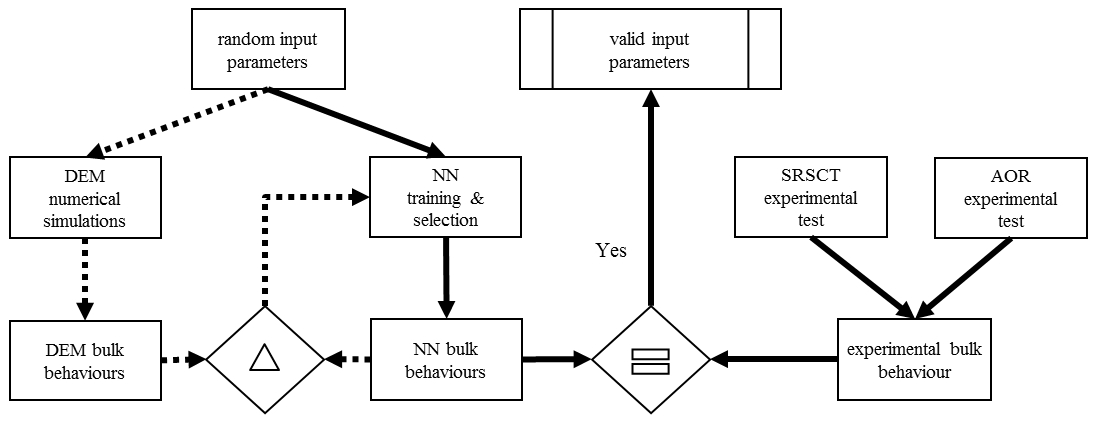
\includegraphics[width=.96\textwidth]{images/019methodology} 
\caption[Method]{Method. In the training phase (dashed lines)
$DEM$ simulations are performed
with random initial input parameters.
The behaviours obtained are used to train the
Artificial Neural Networks ($ANNs$) in a loop that continues until the
difference between the outputs of each $ANN$ and its simulations is below the
limit ($\Delta$).
In the parameters identification phase (solid
lines) we identify valid input parameters by comparing (\textbf{=}) $ANNs$ and
experimental behaviours.}
\label{fig:019methodology} 
\end{figure}

We obtained for each of the twelve load conditions of the \acs{SCT} three bulk
values (\acs{mupsh}, \acs{mush} and \acs{rhob}).
The fourth bulk value was the result of two angle of repose (\acs{AoR}) tests that
recreated the repose angle observed in a pile of the
real material. 
Subsequently, we compared the \acs{ANN} and experimental bulk behaviours for the
twelve shear-cell load conditions.
If in a DEM-parameter combination all the three bulk values differed by less 
than 5\% from those of the corresponding experiments, i.e.:
%************************************************
\begin{equation}
 \begin{cases}
\text{if } & \lvert{1-\frac{\mu_{psh,num}}{\mu_{psh,exp}}}\rvert < 5\%  ,\\
\text{and if } & \lvert{1-\frac{\mu_{sh,num}}{\mu_{sh,exp}}}\rvert < 5\% , \\ 
\text{and if } & \lvert{1-\frac{\rho_{p,num}}{\rho_{p,exp}}}\rvert < 5\% ,\\ 
\end{cases}
 \label{eq:check2}
\end{equation}
the combination was marked. The marked combinations were processed by the
\acs{AoR} \acs{ANN}, and then compared with the experiment.
Were considered valid those that differed by less than $5\%$ also in this
comparison (Eq. \ref{eq:checkaor}):
%************************************************
\begin{equation}
\text{if} ~~~~~~ \lvert{1-\frac{AoR_{num}}{AoR_{exp}}}\rvert < 5\% .
\label{eq:checkaor}
\end{equation}
%************************************************
Further, to prove the validity of the system, we tested the marked combinations
by modifying the experimental bulk values of the shear cell. 
We artificially decreased or increased the shear force, and thus \acs{mupsh} and
\acs{mush}, by a product coefficient ($P$), e.g. Eq. \ref{eq:pcoeff}:
%************************************************
\begin{equation}
\label{eq:pcoeff}
\mu_{psh, new} = \mu_{psh, old} \cdot P .
\end{equation}


\subsection{Value representation}
\label{subsec:valuerepresentation}

\begin{itemize}
  \item{parameter space plot;}
  \item{box plot;
  \improvement{explain about 25 and 75 percentile}
  }
  \item{density plot.}
\end{itemize}

%************************************************
%************************************************

\subsection{SCT parameter space for Sinter fine}
\label{subsec:sctparameterspace}

Experimental values identifying the bulk behavior, \acs{mupsh}, \acs{mush} and $\rho_{b}$, 
of sinter fine were acquired through \acs{SCT} tests. 
Table \ref{tab:05sinterTableExperimental} presents
these values for three load conditions: clearly the \acs{mupsh} decreases, and 
the \acs{mush} oscillates.
The \acs{rhob} has a clear average of 1,760 $kg/m^3$ with a 42 
$kg/m^3$ deviation.
Two \acs{AoR} tests were performed that gave an average angle of
38.85$^\circ$.
We obtained the radius (\acs{R}) mean and standard
deviations, as shown in Table
\ref{tab:09DEMFixedinputvalues}, from sieving experiments.
\wrong{description of 1068 is missing.}
The comparison between numerical and experimental behaviours led to a first
series of marked combinations ($MC1$) for one load condition of
the shear cell ($\acs{sigman} = 10,070$ Pa, P=1.0), as plotted in Fig.
\ref{fig:024radarpirker1schulze10070}, where 
the minimum and maximum values are shown, together with the mean. 
Each axis of the parameter space plot represents one simulation parameter.
The shaded area indicates valid parameter combinations, and dark shaded
values indicate the confidence range.
Note that the confidence interval is large, 
especially for the \acs{CoR}, which highlights its insignificant influence on the
characterization.
Both the \acs{rhop}  and the \acs{mus}, however, show a narrow confidence interval, 
which demonstrates their influence and the ability of this procedure to find
valid \acs{DEM} parameters.
These results agree with our examination of the ratio of the standard deviation
to the range, see Table \ref{tab:13DEMvalidvalues}.

\subsection{SCT cloud space}
\label{subsec:sctcloudspace}

Further, we observed that various \acs{DEM} parameter
combinations could reproduce the experimental behaviour, and thus evaluated
their mutual dependencies.
This is shown more clearly in a density plot (see Fig. 
\ref{fig:025cloudpirker1schulze10070} for $MC1$) 
of the particles' coefficient of restitution (\acs{CoR}) in relation to
the coefficients of sliding friction (\acs{mus}) and rolling friction (\acs{mur}); 
in the white area, no valid sets of simulation parameters could be found.
In each cell the valid sets are grouped according to the 4 different COR
ranges.
Each cell is coloured according to the group with the most members.
Multiple
combinations (250,407 or 4\% of the total) of \acs{mus} and \acs{mur} reproduced
the experimental behaviour with varying \acs{CoR}.
This underlines once more their correlation, as already stated by Wensrich and 
Katterfeld \cite{RefWorks:87}.
To further demonstrate the validity of the procedure, we modified the product
coefficient. 
First, we set it to $P=0.8$, and we obtained another
series of marked combinations ($MC2$).
It could be seen in the parameter space plot in Fig.
\ref{fig:026radarpirker08schulze10070} that the confidence range is narrower
than for $P=1.0$, while in the density plot in Fig. 
\ref{fig:027cloudpirker08schulze10070} the area
appears larger, although slightly less densely populated. Finally, for $P=1.2$
and its marked combinations ($MC3$) the parameter space plot in Fig.
\ref{fig:028radarpirker12schulze10070} shows a largely different confidence
range, while the density plot in Fig. \ref{fig:030cloudpirker12schulze10070} 
shows a smaller area. As expected, the procedure was highly sensitive to
variations in the experimental data.
Our approach could therefore be used
for a wide range of bulk materials.\\

\subsection{AoR and merge results}
\label{subsec:aorandmergeresults}

We then processed the random combinations with the \acs{AoR} \acs{ANN}. In Fig.
\ref{fig:031radarpirker1aor} the parameter space plot for the same criteria as
before could be seen.
In accordance with theory (Wensrich and Katterfeld \cite{RefWorks:87}), in a simulation dominated
by rolling particles, the coefficient of rolling friction has the maximum
influence. \\
Finally, we extracted from the $MC1$ values the \acs{AoR} \acs{ANN} behaviour
and compared it with the experimental one.
As could be seen in the parameter space plot in Fig.
\ref{fig:033radarpirker1schulze10070aor}, the confidence interval is very small,
indicating that all the parameters but the \acs{CoR} played an important role, 
and demonstrating the reliability of these parameter
combinations in representing the bulk behaviour.
From the initial 6,250,000 combinations, only 3,884 were valid (0.0621
\%), see Table \ref{tab:13DEMvalidvalues}.
%************************************************
\begin{table}[h]
\centering
\begin{tabular}{cccccc}
\hline
$\sigma_n$ (Pa) & $\tau$ (Pa) & $\mu_{psh}$ (-) & $\tau_{\%}$ (\%) &
$\mu_{sh}$ (-) & $\rho_b$ (kg/m3) \\
\hline
    1068  & 1059  & 0.9916 & 80 & 1.2333 & 1718 \\
    2069  & 1818  & 0.8787 & 80 & 0.9994 & 1759 \\
    10070 & 8232  & 0.8175 & 80 & 1.1712 & 1802 \\

\hline
\end{tabular}
\caption[Experimental results]{Experimental results. Values for three
load conditions}
\label{tab:05sinterTableExperimental}
\end{table}
\info{one table for each material? here or in the polydispersity chapter?}

\begin{table}[h]
\centering
\begin{tabular}{llccc}
\hline

          & type  & SSC & AoR   & SSC \& AoR \\
          \hline

    $\mu_s$ & mean  & 0.831 & 0.177 & 0.664 \\
    $[-]$   & std. dev. (SD) & 0.097 & 0.095 & 0.029 \\
          & range ($R$) & 0.9   & 0.9   & 0.9 \\
          & SD / R & 0.108 & 0.106 & 0.032 \\
          \hline
    $\mu_r$ & mean  & 0.692 & 0.830 & 0.916 \\
    $[-]$   & std. dev. (SD) & 0.215 & 0.193 & 0.042 \\
          & range ($R$) & 0.9   & 0.9   & 0.9 \\
          & SD / R & 0.239 & 0.214 & 0.046 \\
          \hline
              COR   & mean  & 0.708 & 0.590 & 0.590 \\
   $ [-]$   & std. dev. (SD) & 0.104 & 0.073 & 0.065 \\
          & range ($R$) & 0.4   & 0.4   & 0.4 \\
          & SD / R & 0.259 & 0.183 & 0.161 \\
          \hline
    $\rho_p$ & mean  & 2245.7 & 3192.8 & 2283.9 \\
    $[kg/m3]$ & std. dev. (SD) & 80.5  & 277.4 & 67.1 \\
          & range ($R$) & 1500  & 1500  & 1500 \\
          & SD / R & 0.054 & 0.185 & 0.045 \\
          \hline
    valid & number & 290203 & 816552 & 3884 \\
    combinations & [$\%$] & 4.64  & 13.06 & 0.06 \\  

\hline
\end{tabular}
\caption[DEM valid values]{DEM valid values. For each parameter we show the
valid parameters statistics in the two tests and in their intersection.
Finally, we show the number of valid parameters combinations over the total
(6250000).}
\label{tab:13DEMvalidvalues}
\end{table}


%************************************************
\begin{figure}[htbp]
\centering 
  \subfloat[Parameter space plot, \acs{SCT}, $\sigma_n=1068$ Pa, P=1.0.]{
	  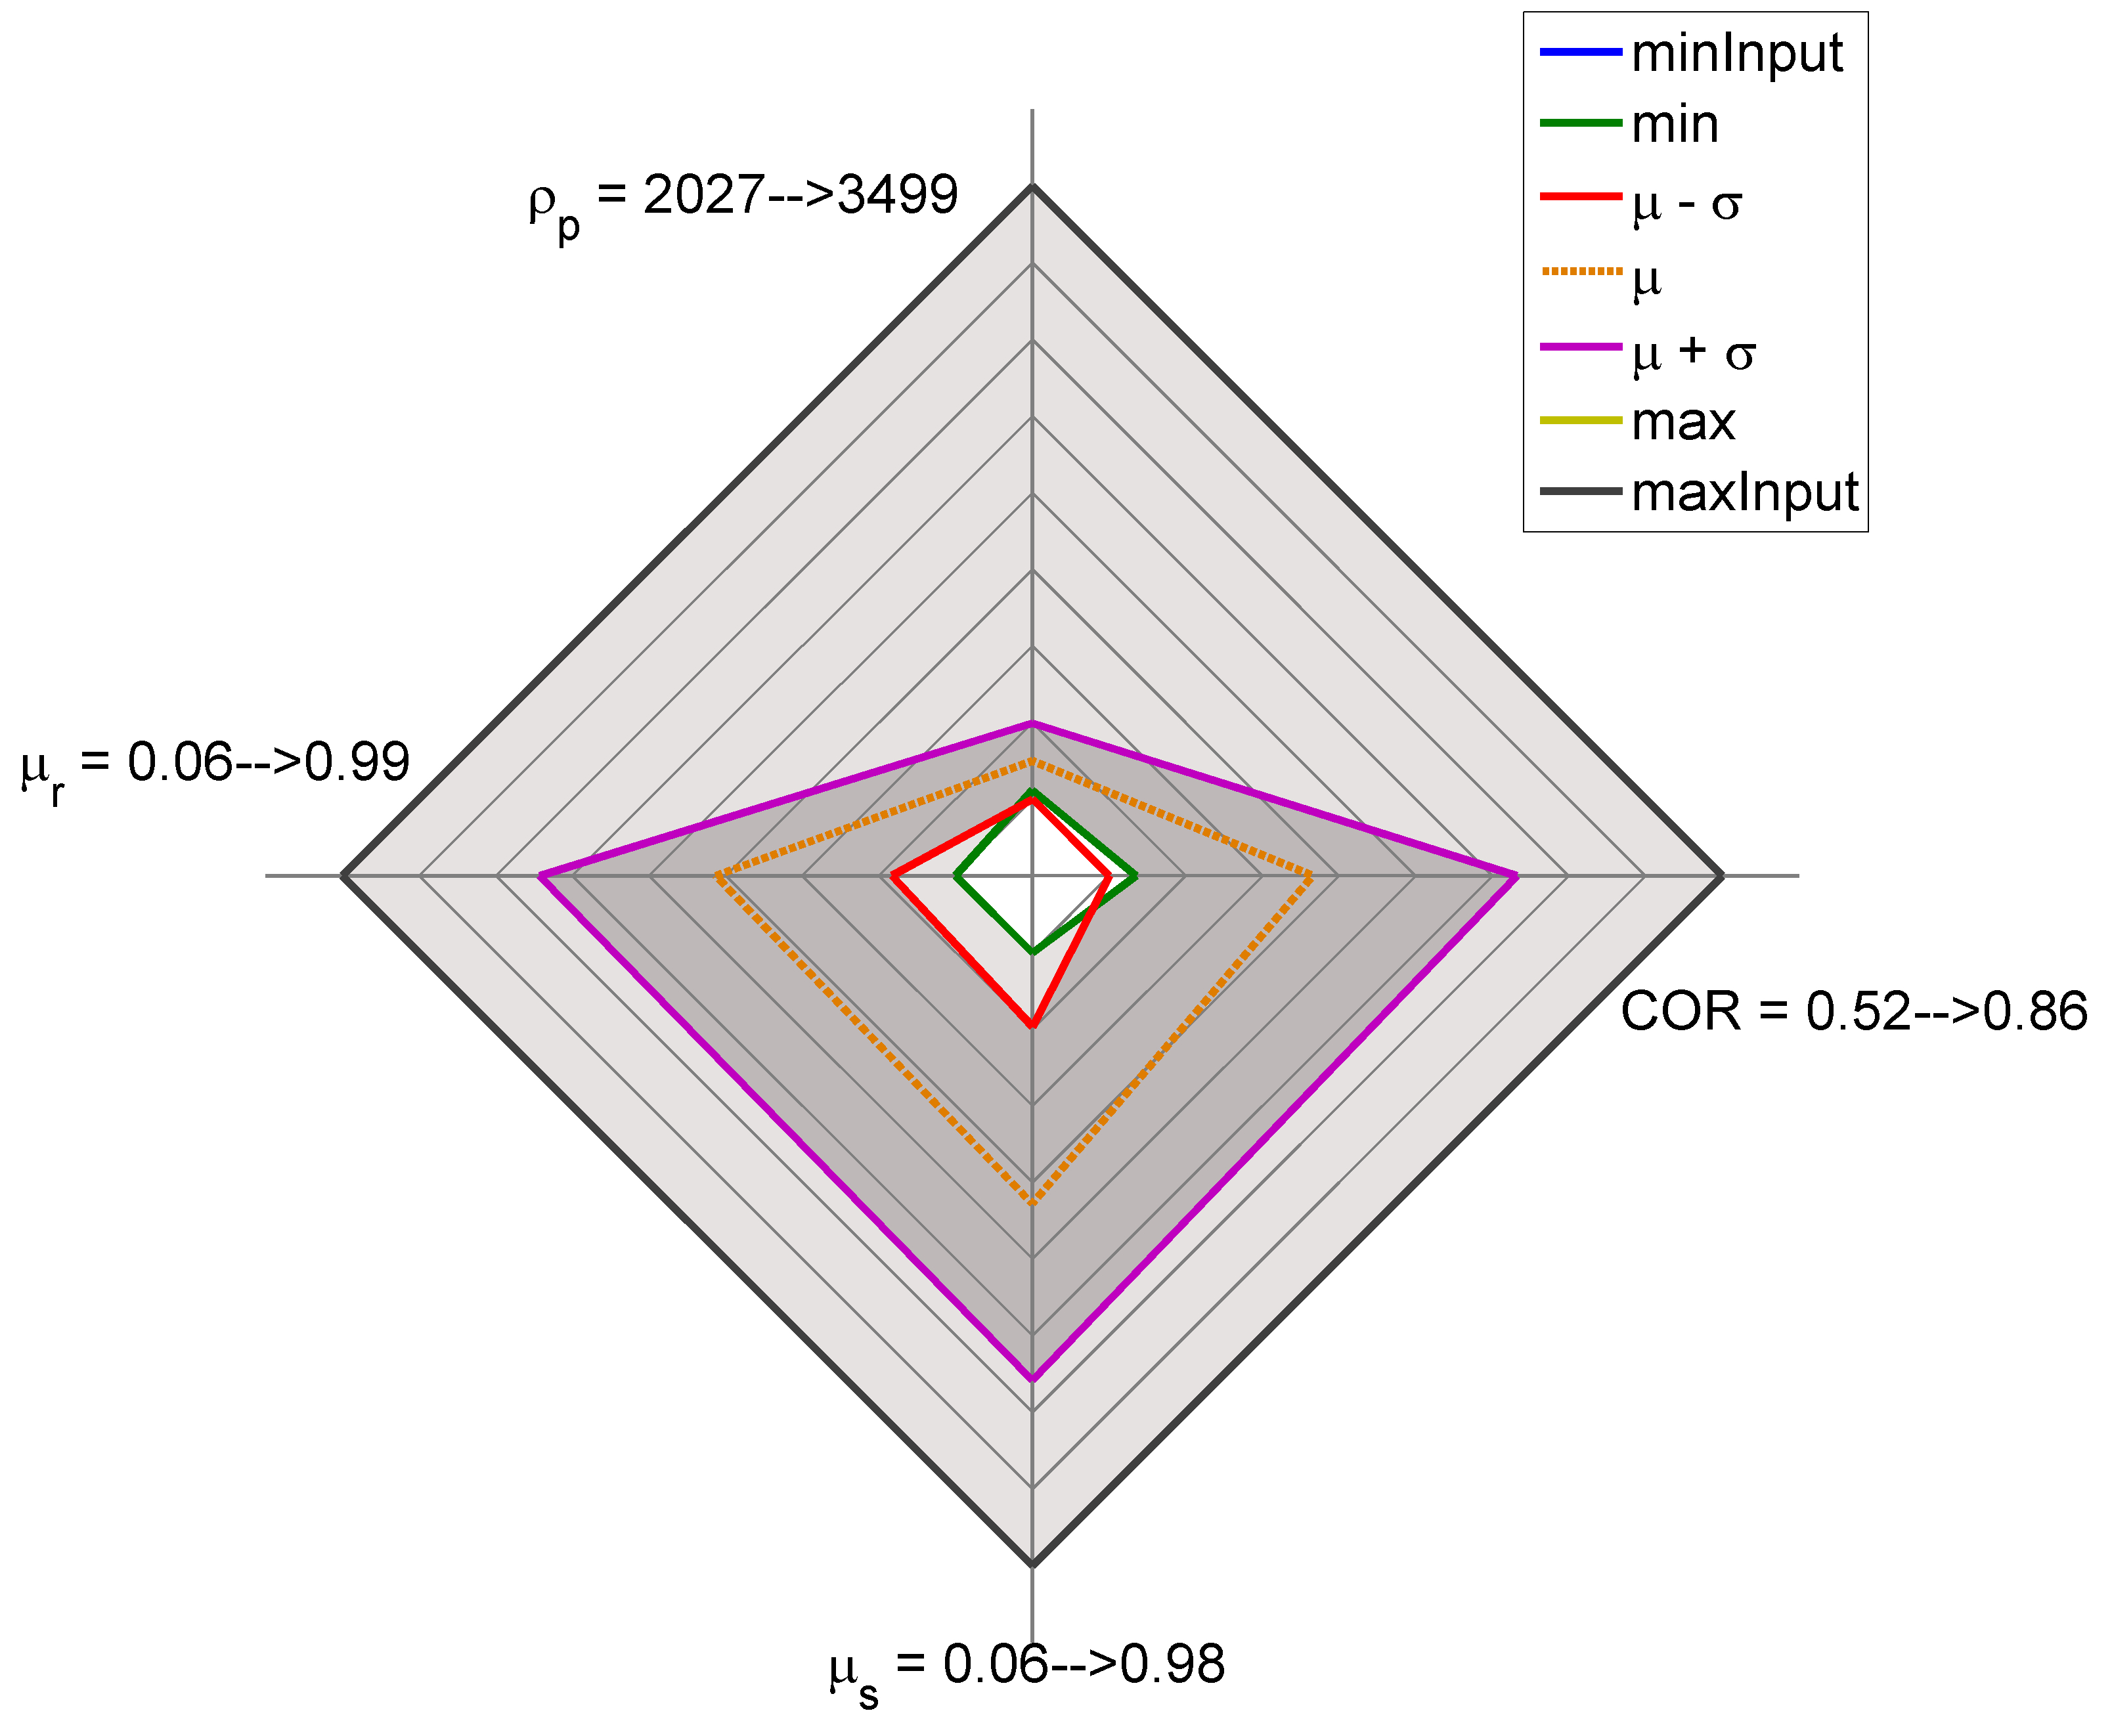
\includegraphics[width=.35\columnwidth]{images/041radarpirker1schulze1068}
	  \label{fig:041radarpirker1schulze1068}
  }
  \\
    \subfloat[Parameter space plot, \acs{SCT}, $\sigma_n=10070$ Pa, P=0.8.]{
	  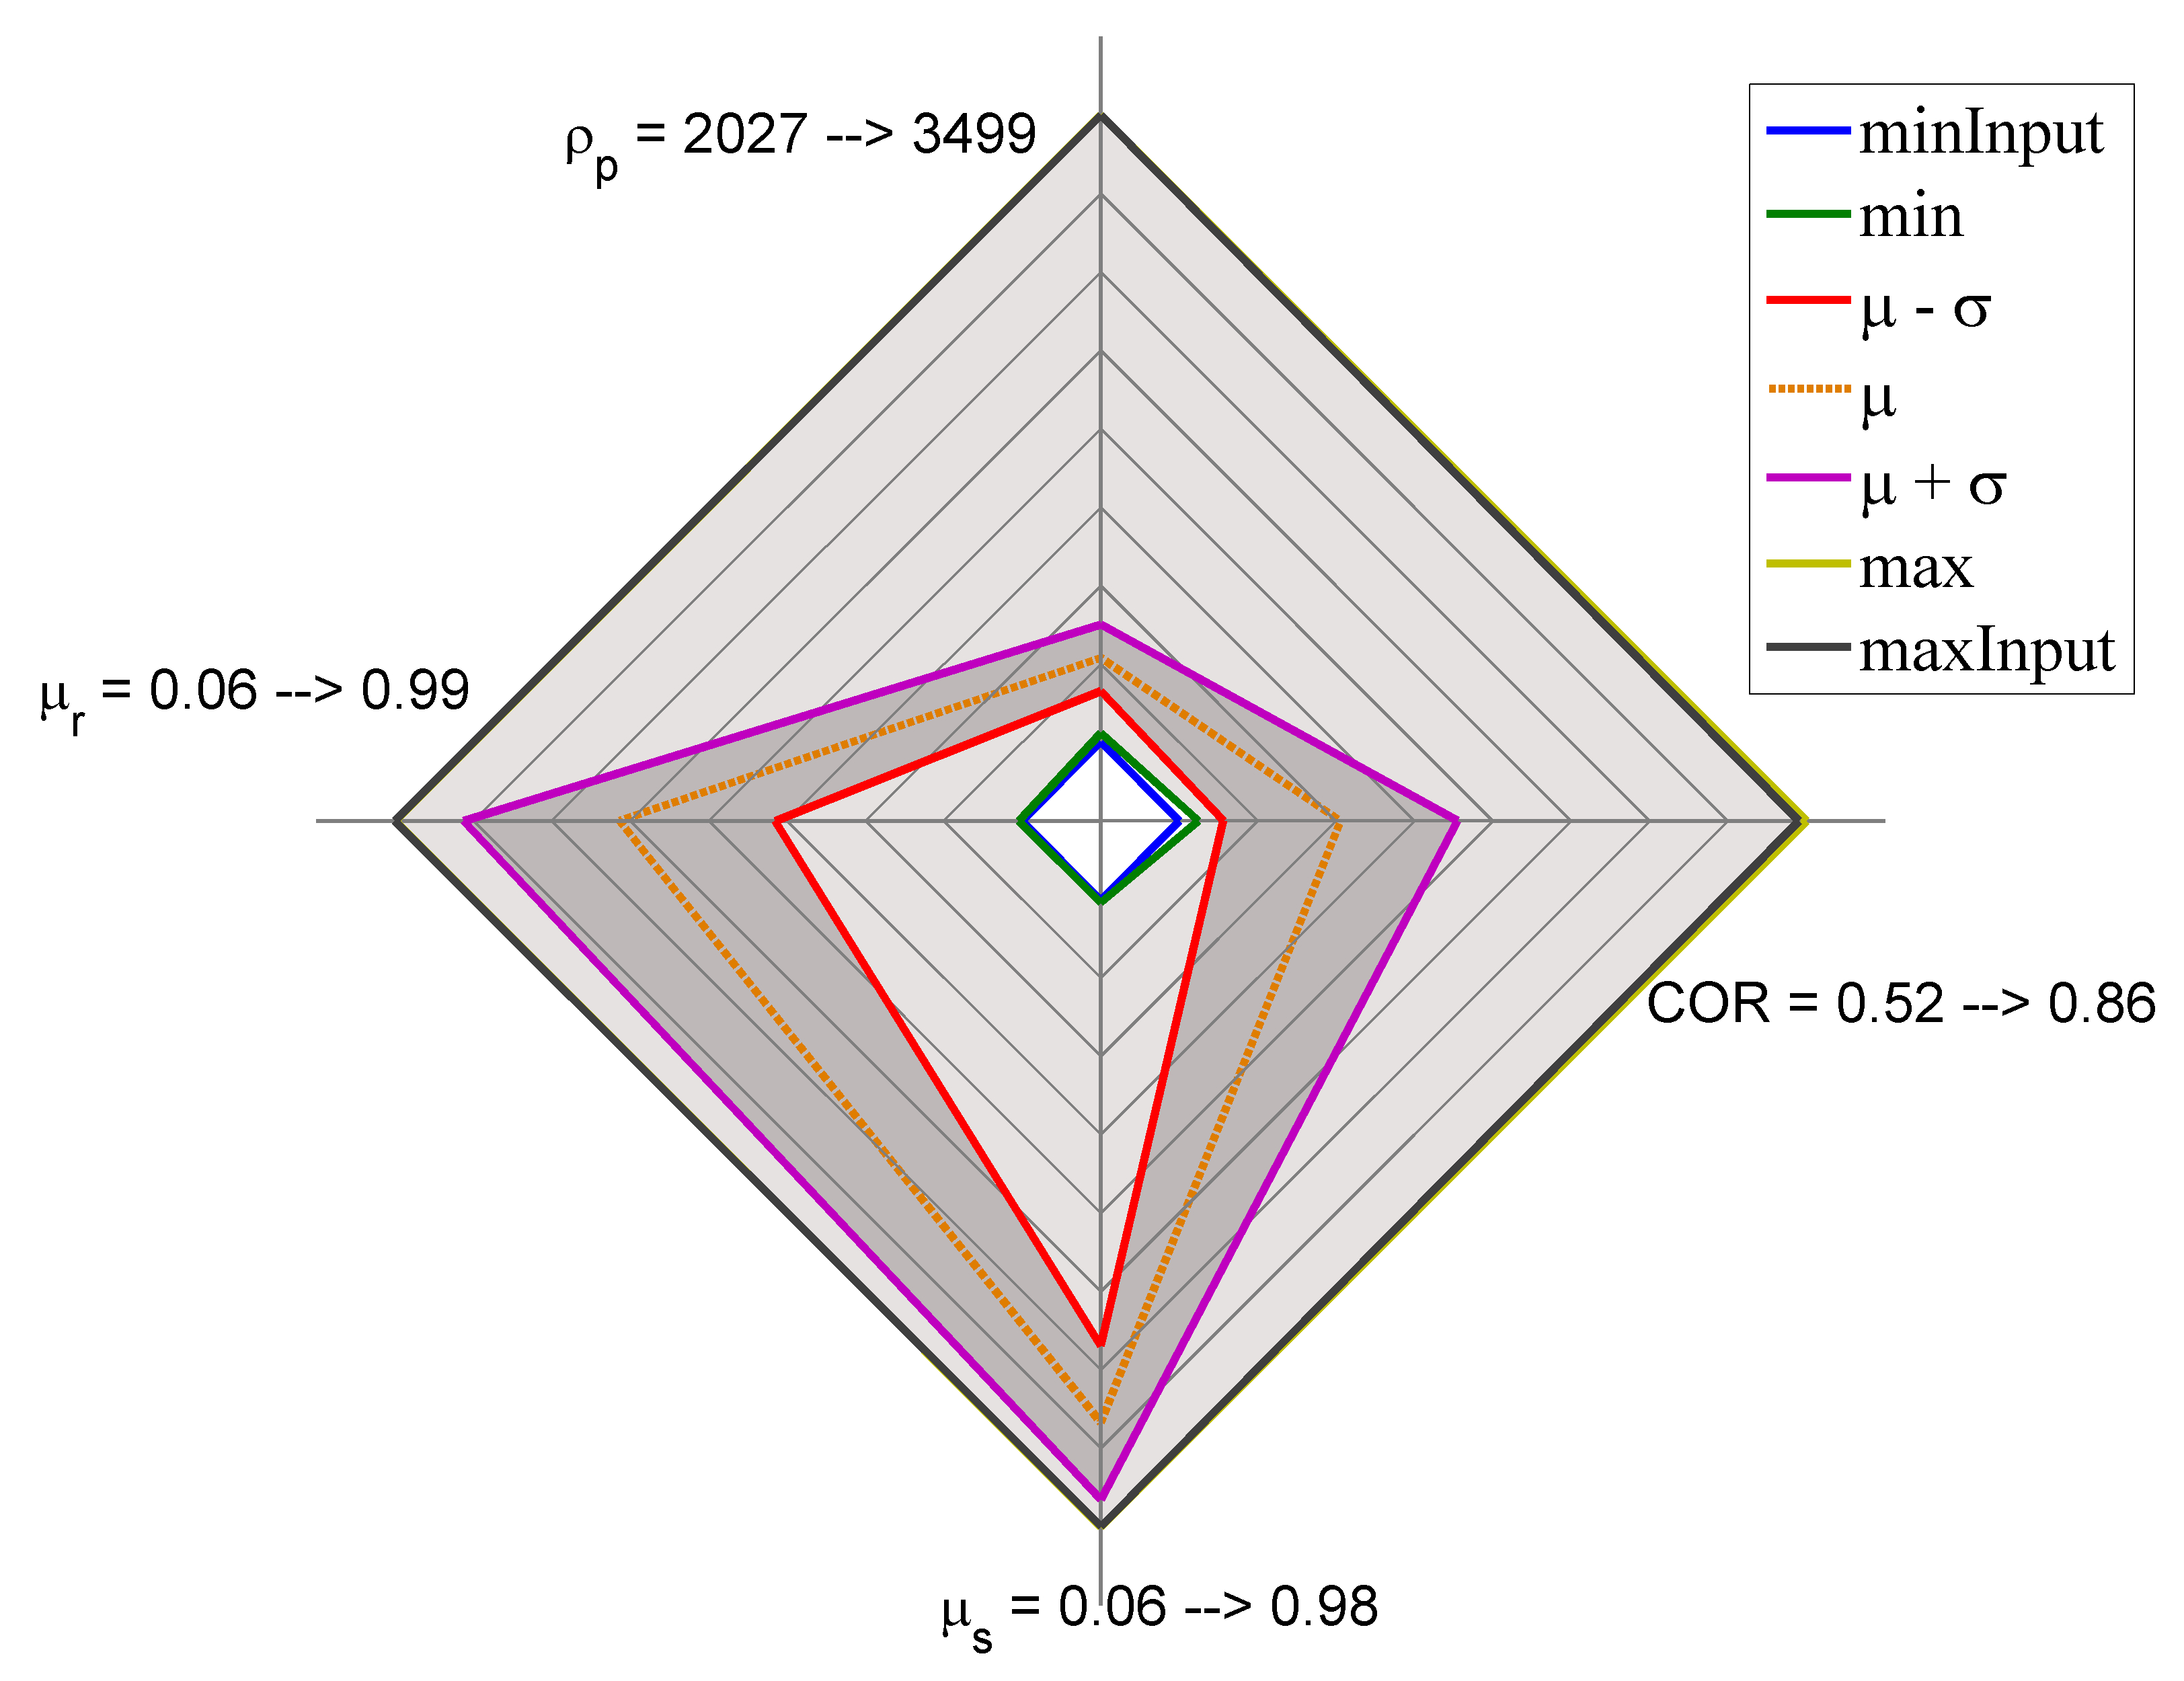
\includegraphics[width=.35\columnwidth]{images/026radarpirker08schulze10070}
	  \label{fig:026radarpirker08schulze10070}
  }
  \\
  \subfloat[Parameter space plot, \acs{SCT}, $\sigma_n=10070$ Pa, P=1.0.]{
	  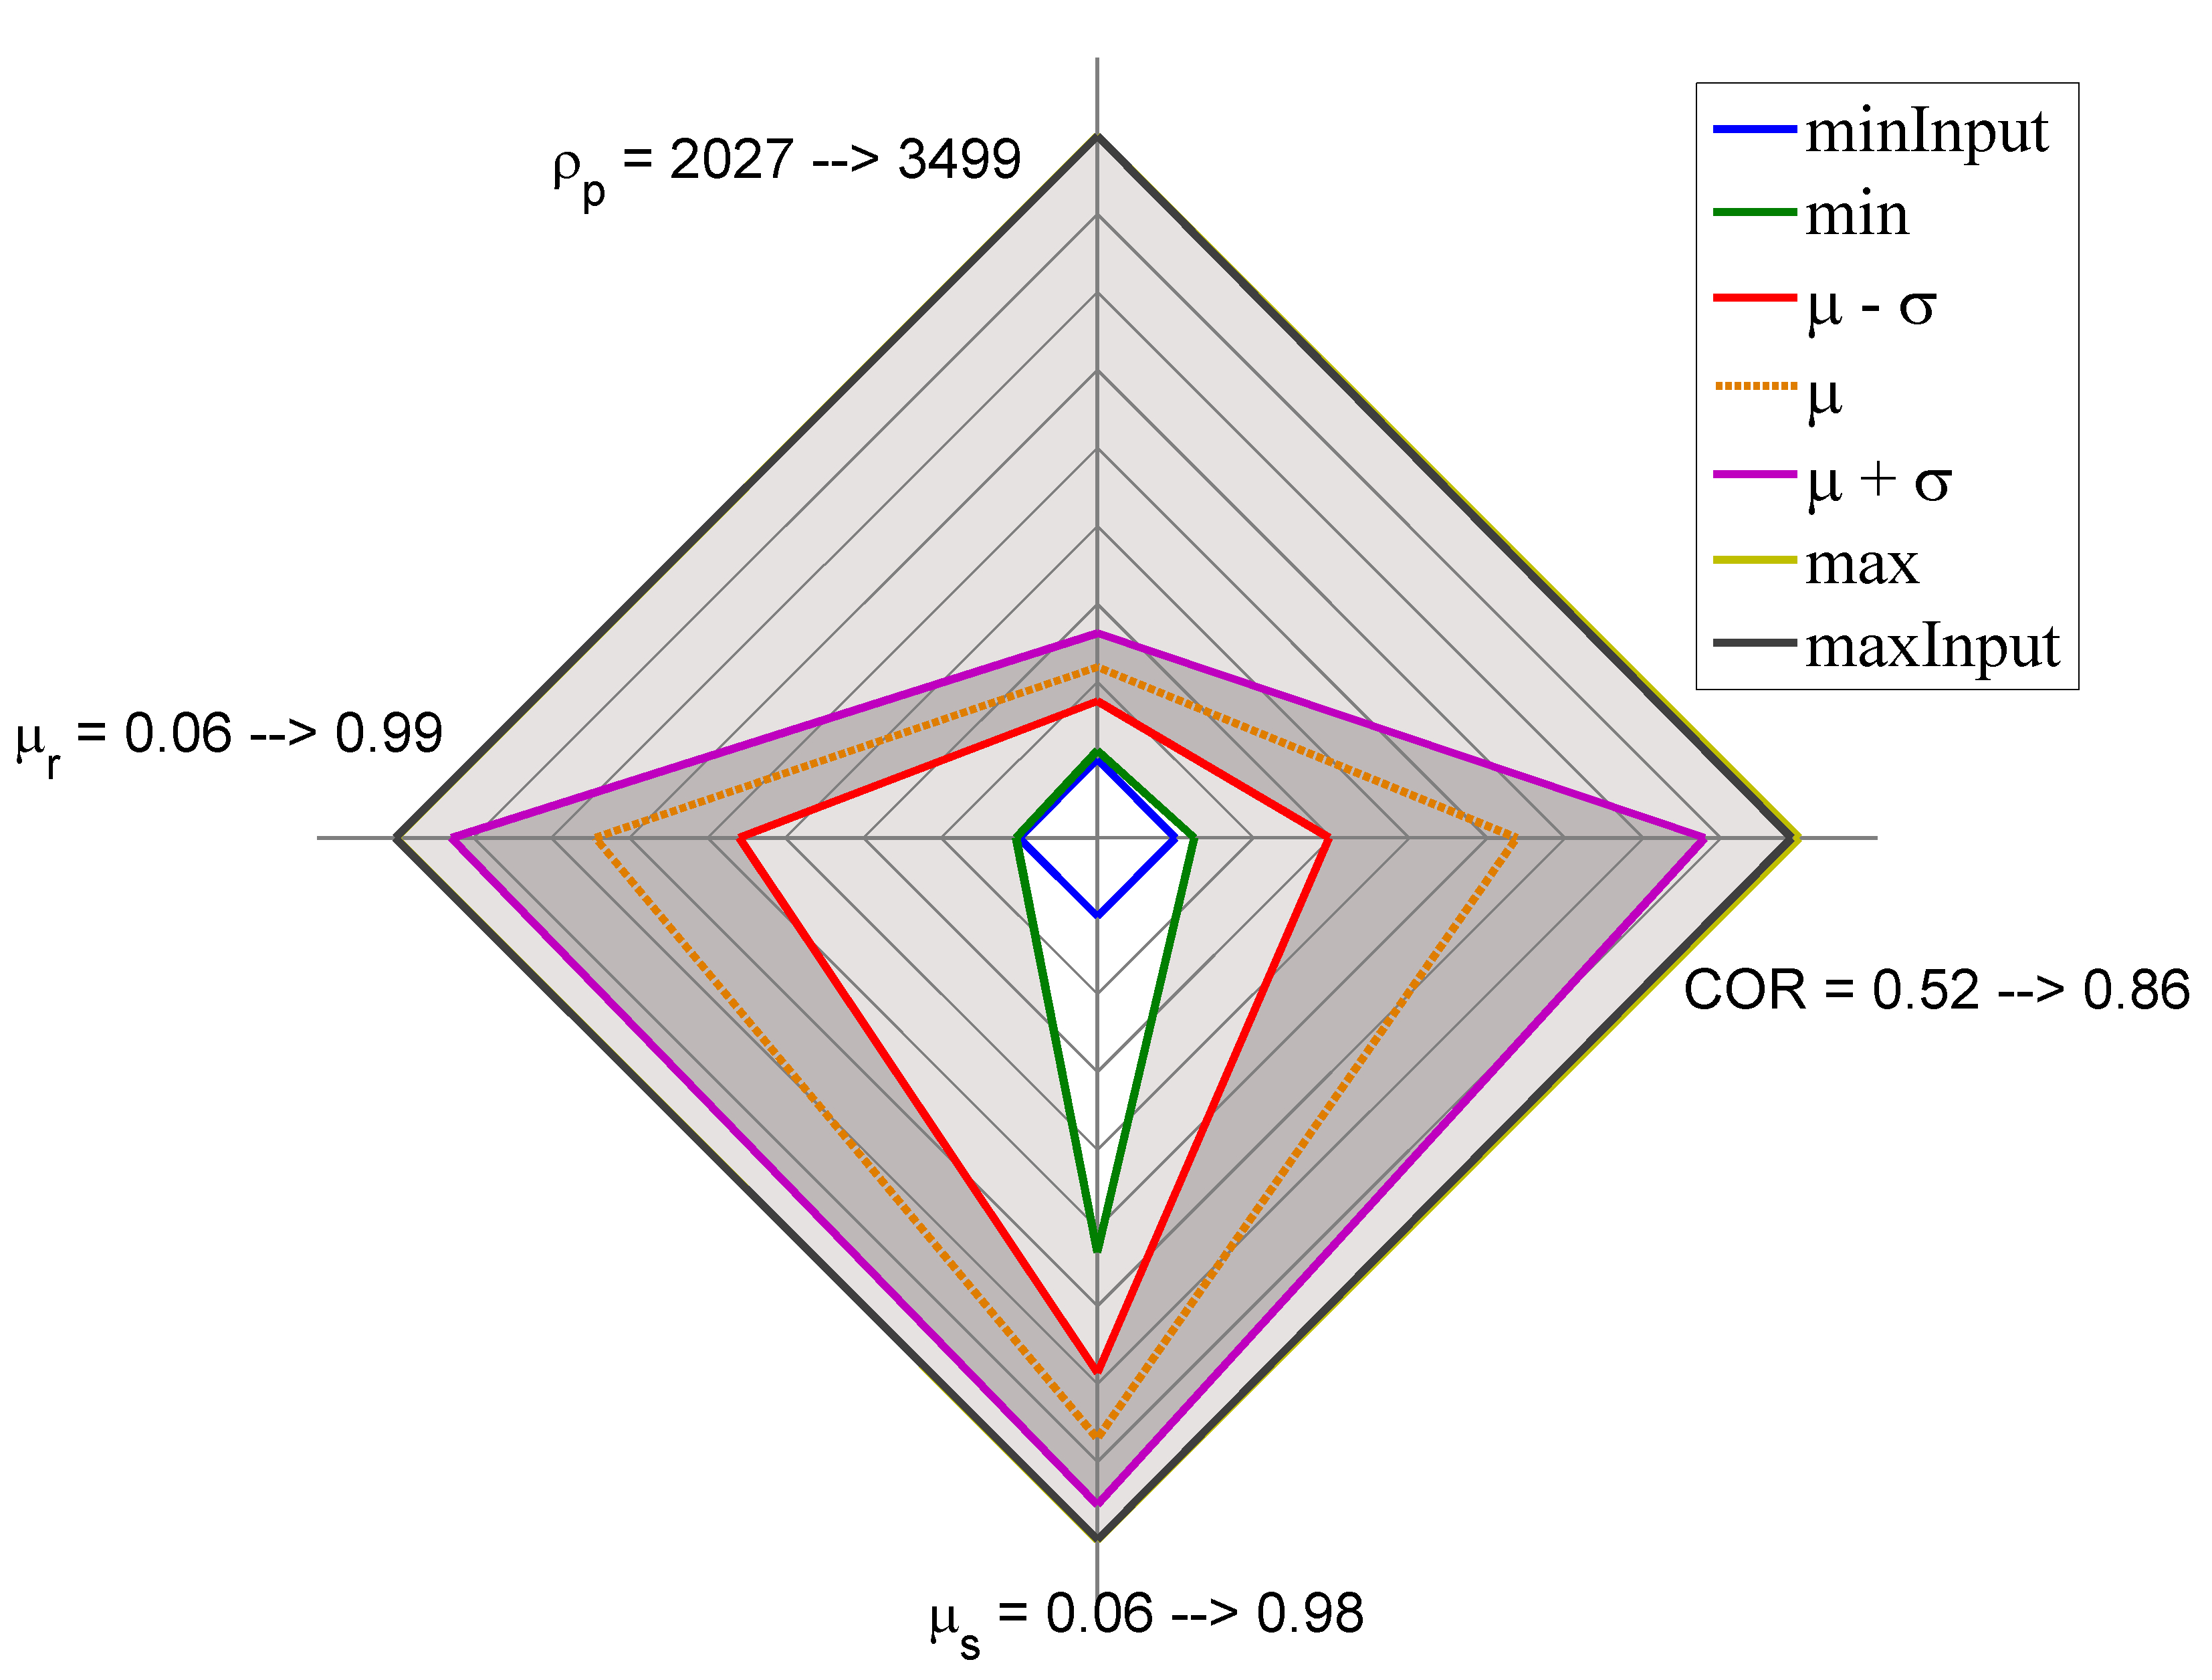
\includegraphics[width=.35\columnwidth]{images/024radarpirker1schulze10070}
	  \label{fig:024radarpirker1schulze10070}
  }
  \quad
    \subfloat[Box plot, \acs{SCT}, $\sigma_n=10070$ Pa, P=1.0.]{
	  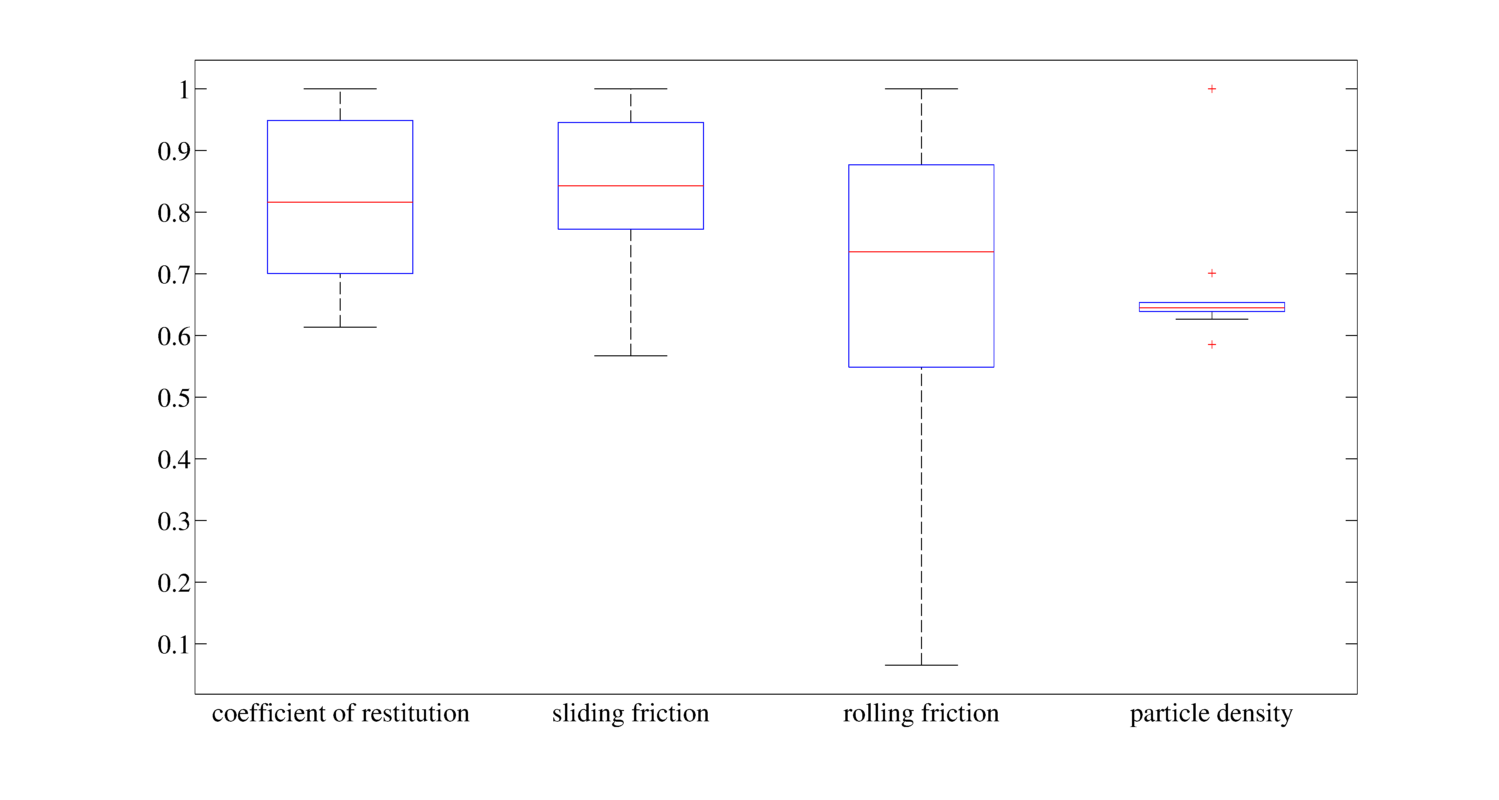
\includegraphics[width=.35\columnwidth]{images/075sctboxplot}
	  \label{fig:075sctboxplot}  }
  \\
    \subfloat[Parameter space plot, \acs{SCT}, $\sigma_n=10070$ Pa, P=1.2.]{
	  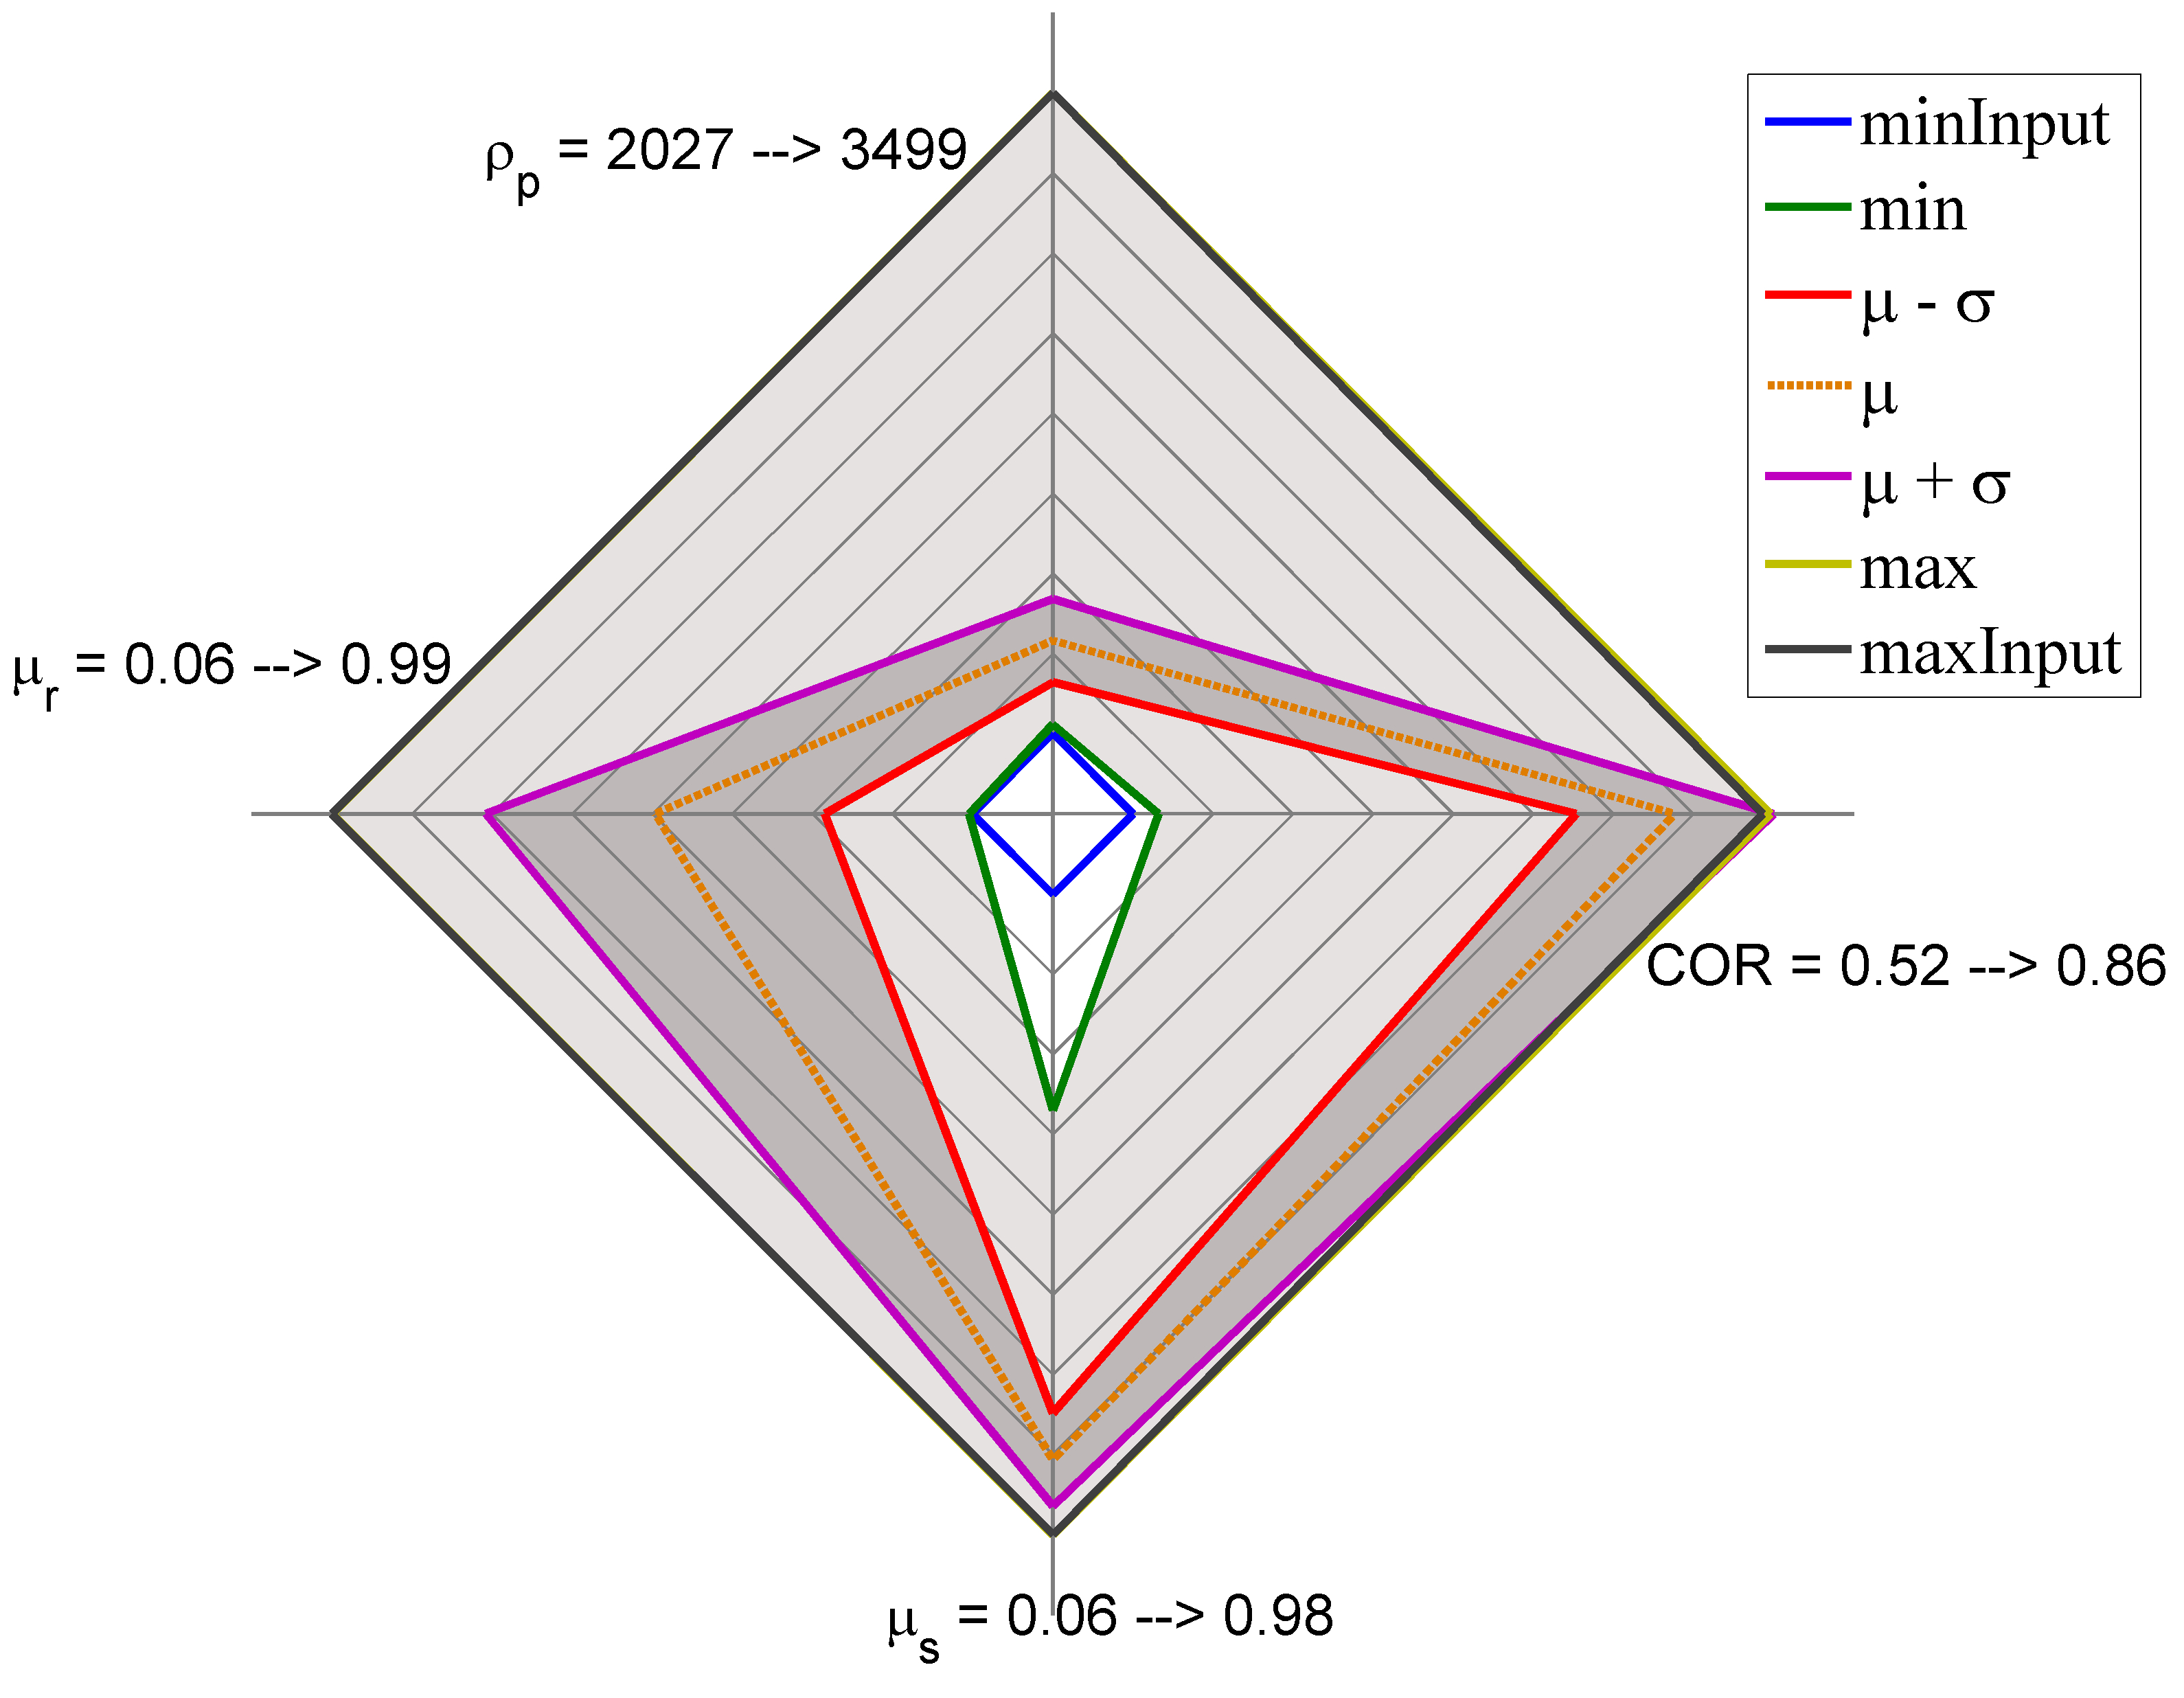
\includegraphics[width=.35\columnwidth]{images/028radarpirker12schulze10070}
	  \label{fig:028radarpirker12schulze10070}
  }
  \caption{SCT parameter space plots.}
  \label{fig:079sctparameterspaceplots}
\end{figure}
\begin{figure}[htbp]
\centering 
  \subfloat[Density plot, $SSC$, $\sigma_n=10070$ Pa, P=0.8.]{
	  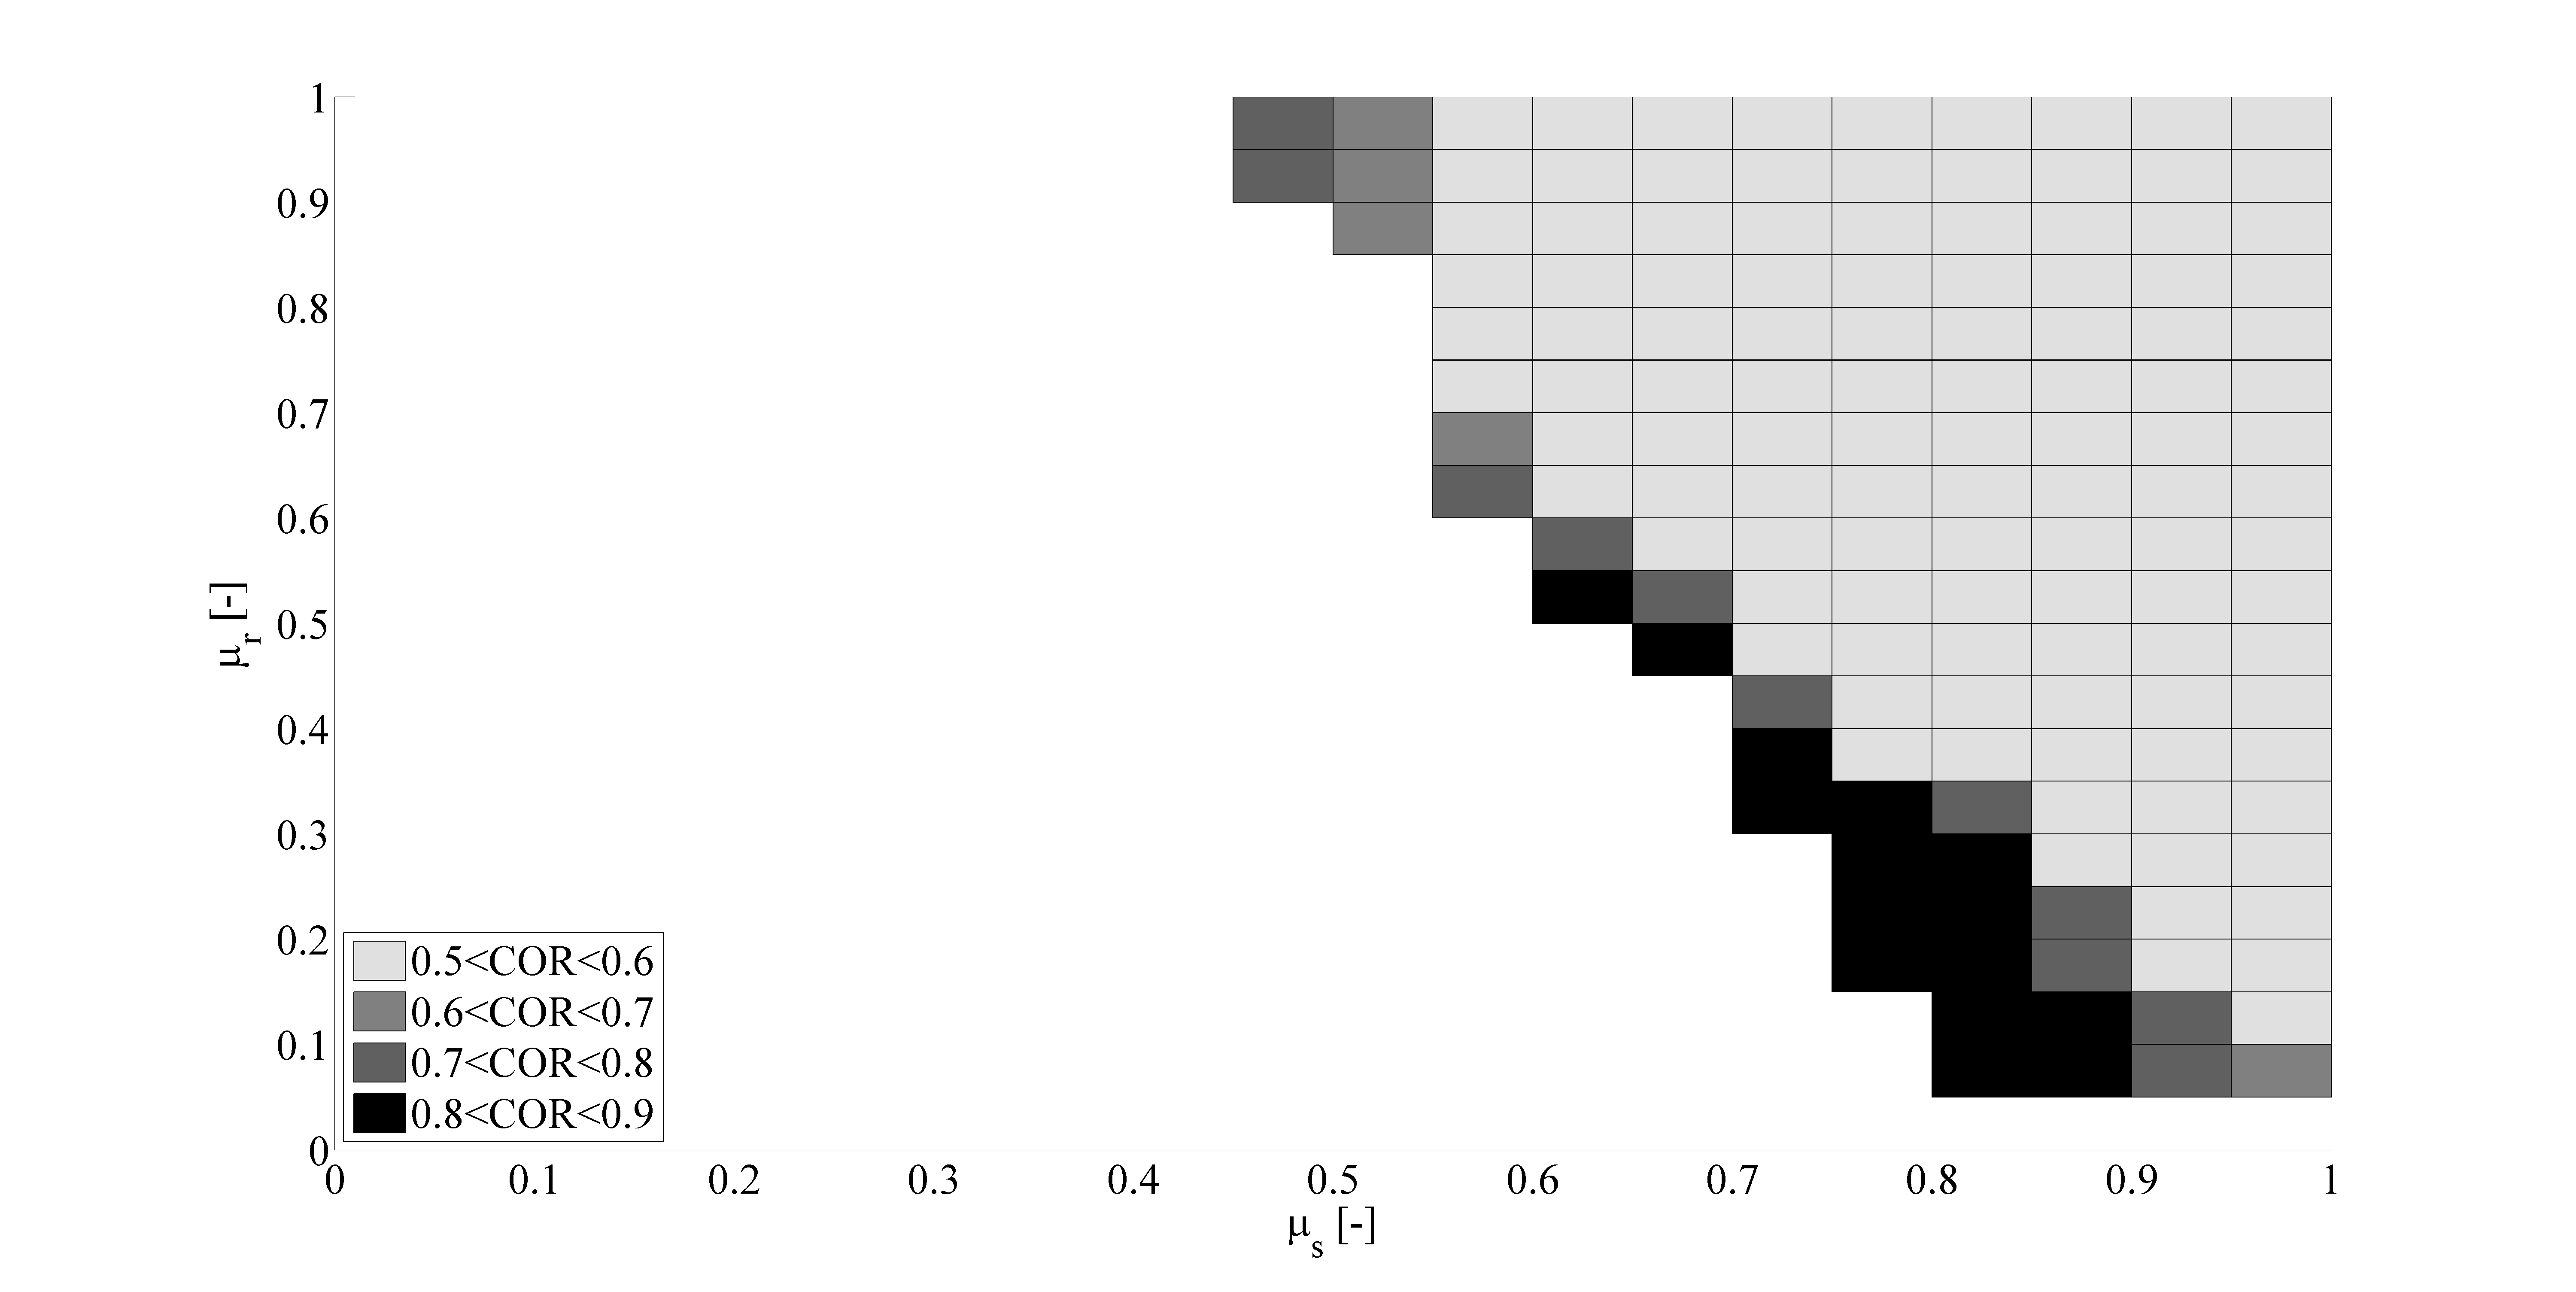
\includegraphics[width=.48\columnwidth]{images/027cloudpirker08schulze10070}
	  \label{fig:027cloudpirker08schulze10070}
  }
  \\
    \subfloat[Density plot, $SSC$, $\sigma_n=10070$ Pa, P=1.0.]{
	  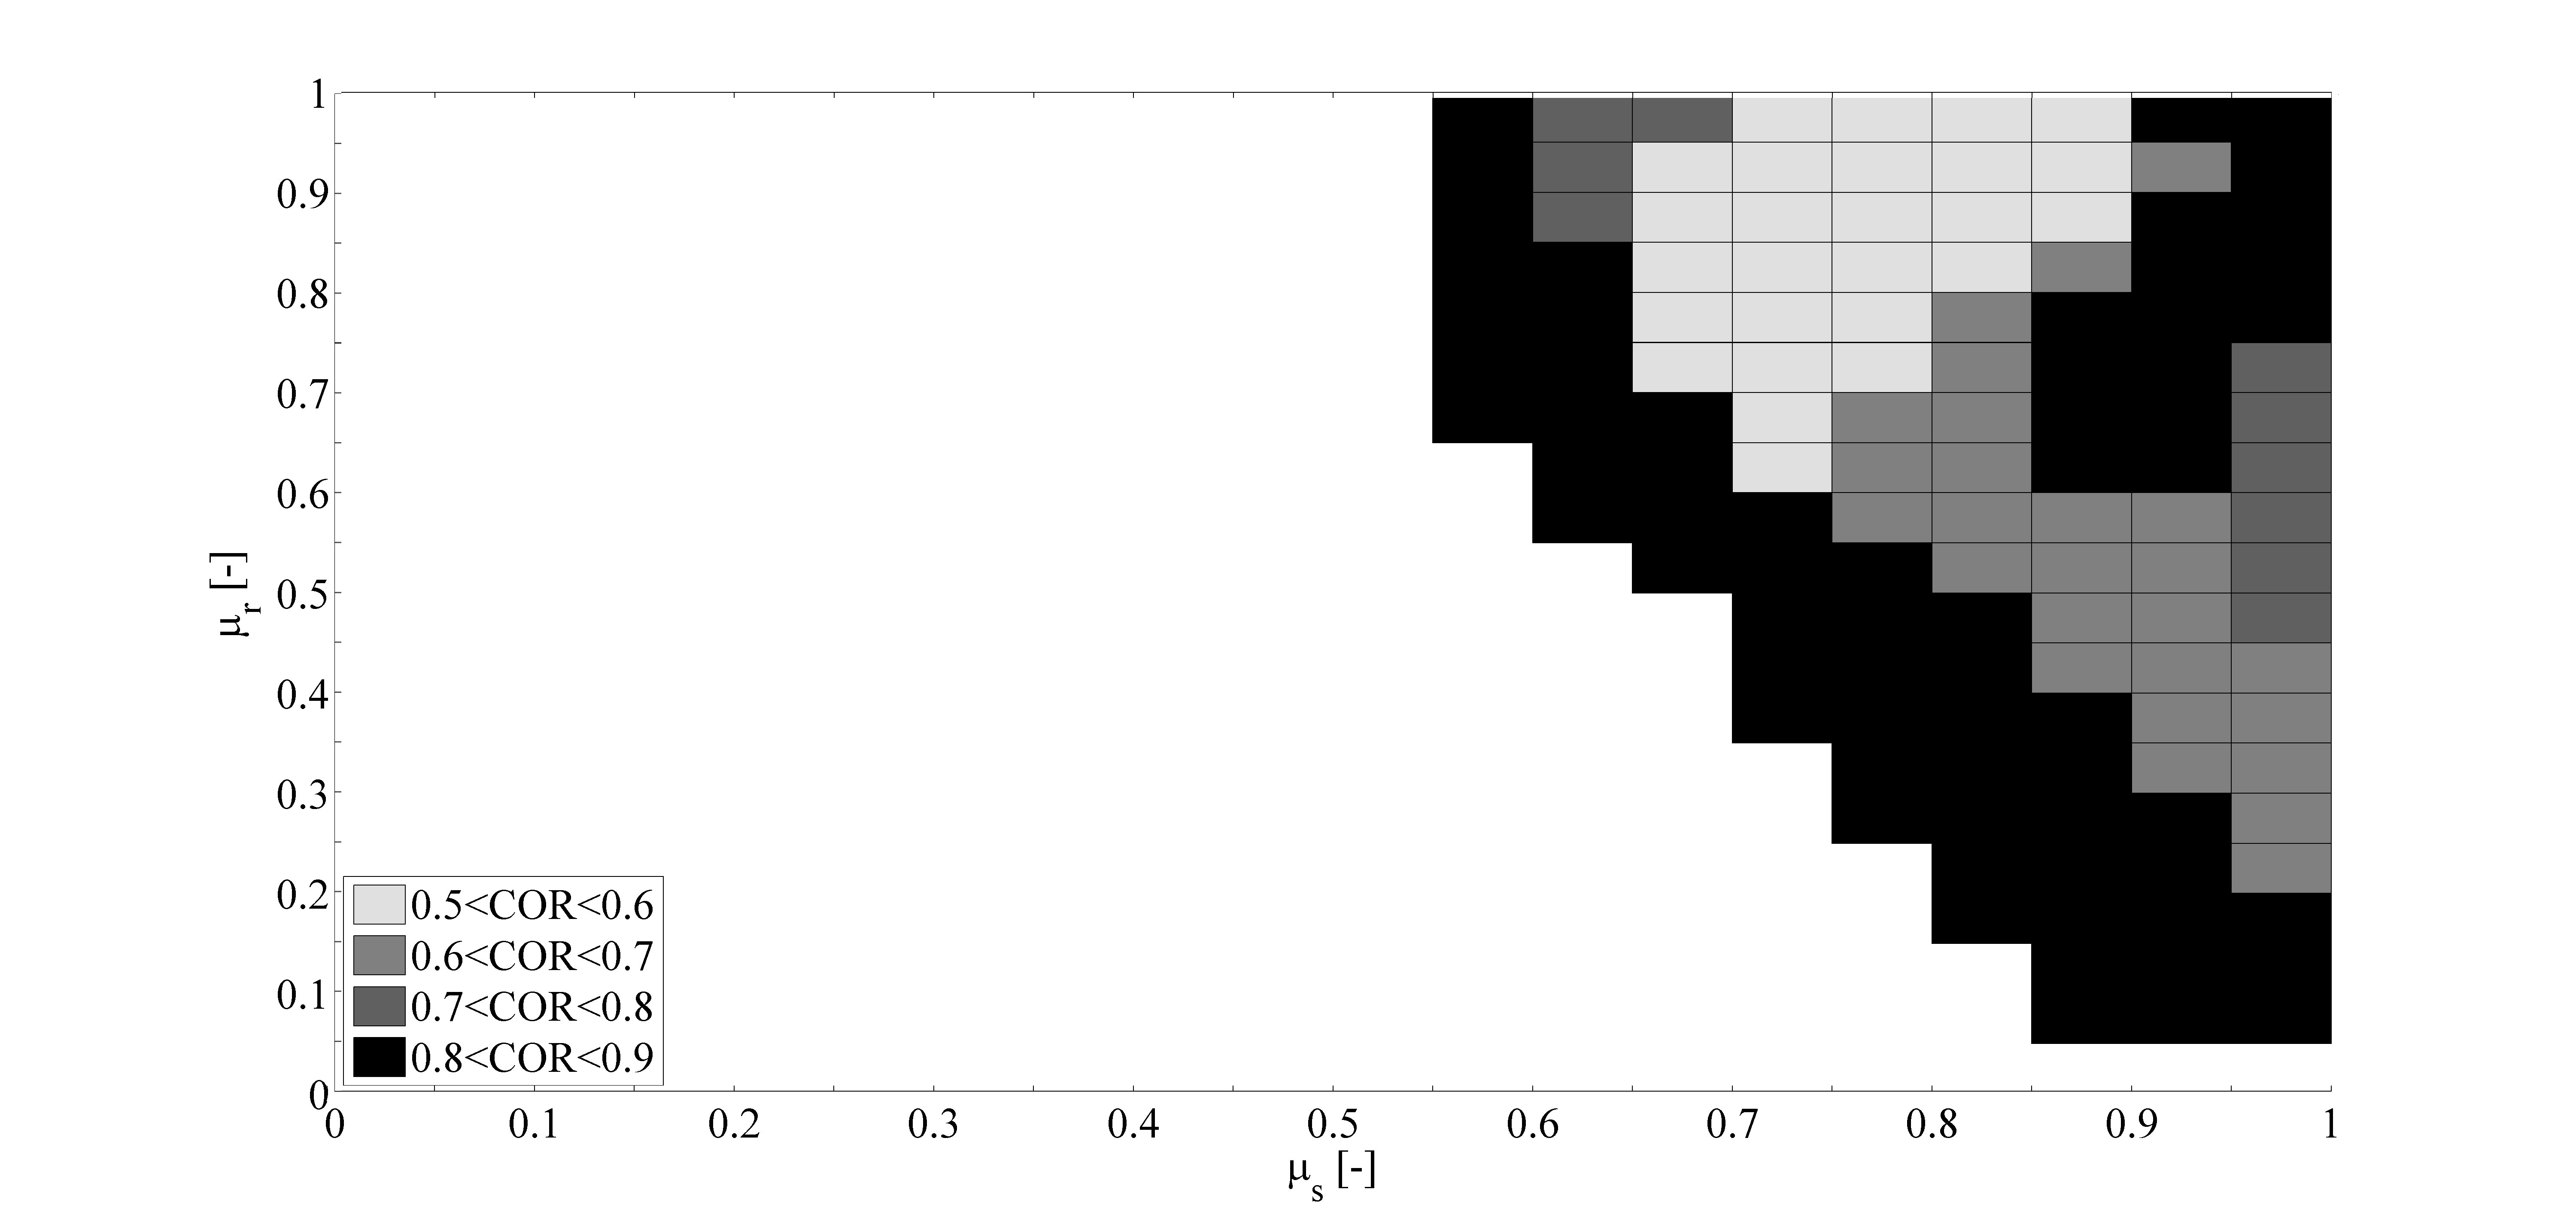
\includegraphics[width=.48\columnwidth]{images/025cloudpirker1schulze10070}
	  \label{fig:025cloudpirker1schulze10070}
  }
  \\
  \subfloat[Density plot, $SSC$, $\sigma_n=10070$ Pa, P=1.2.]{
	  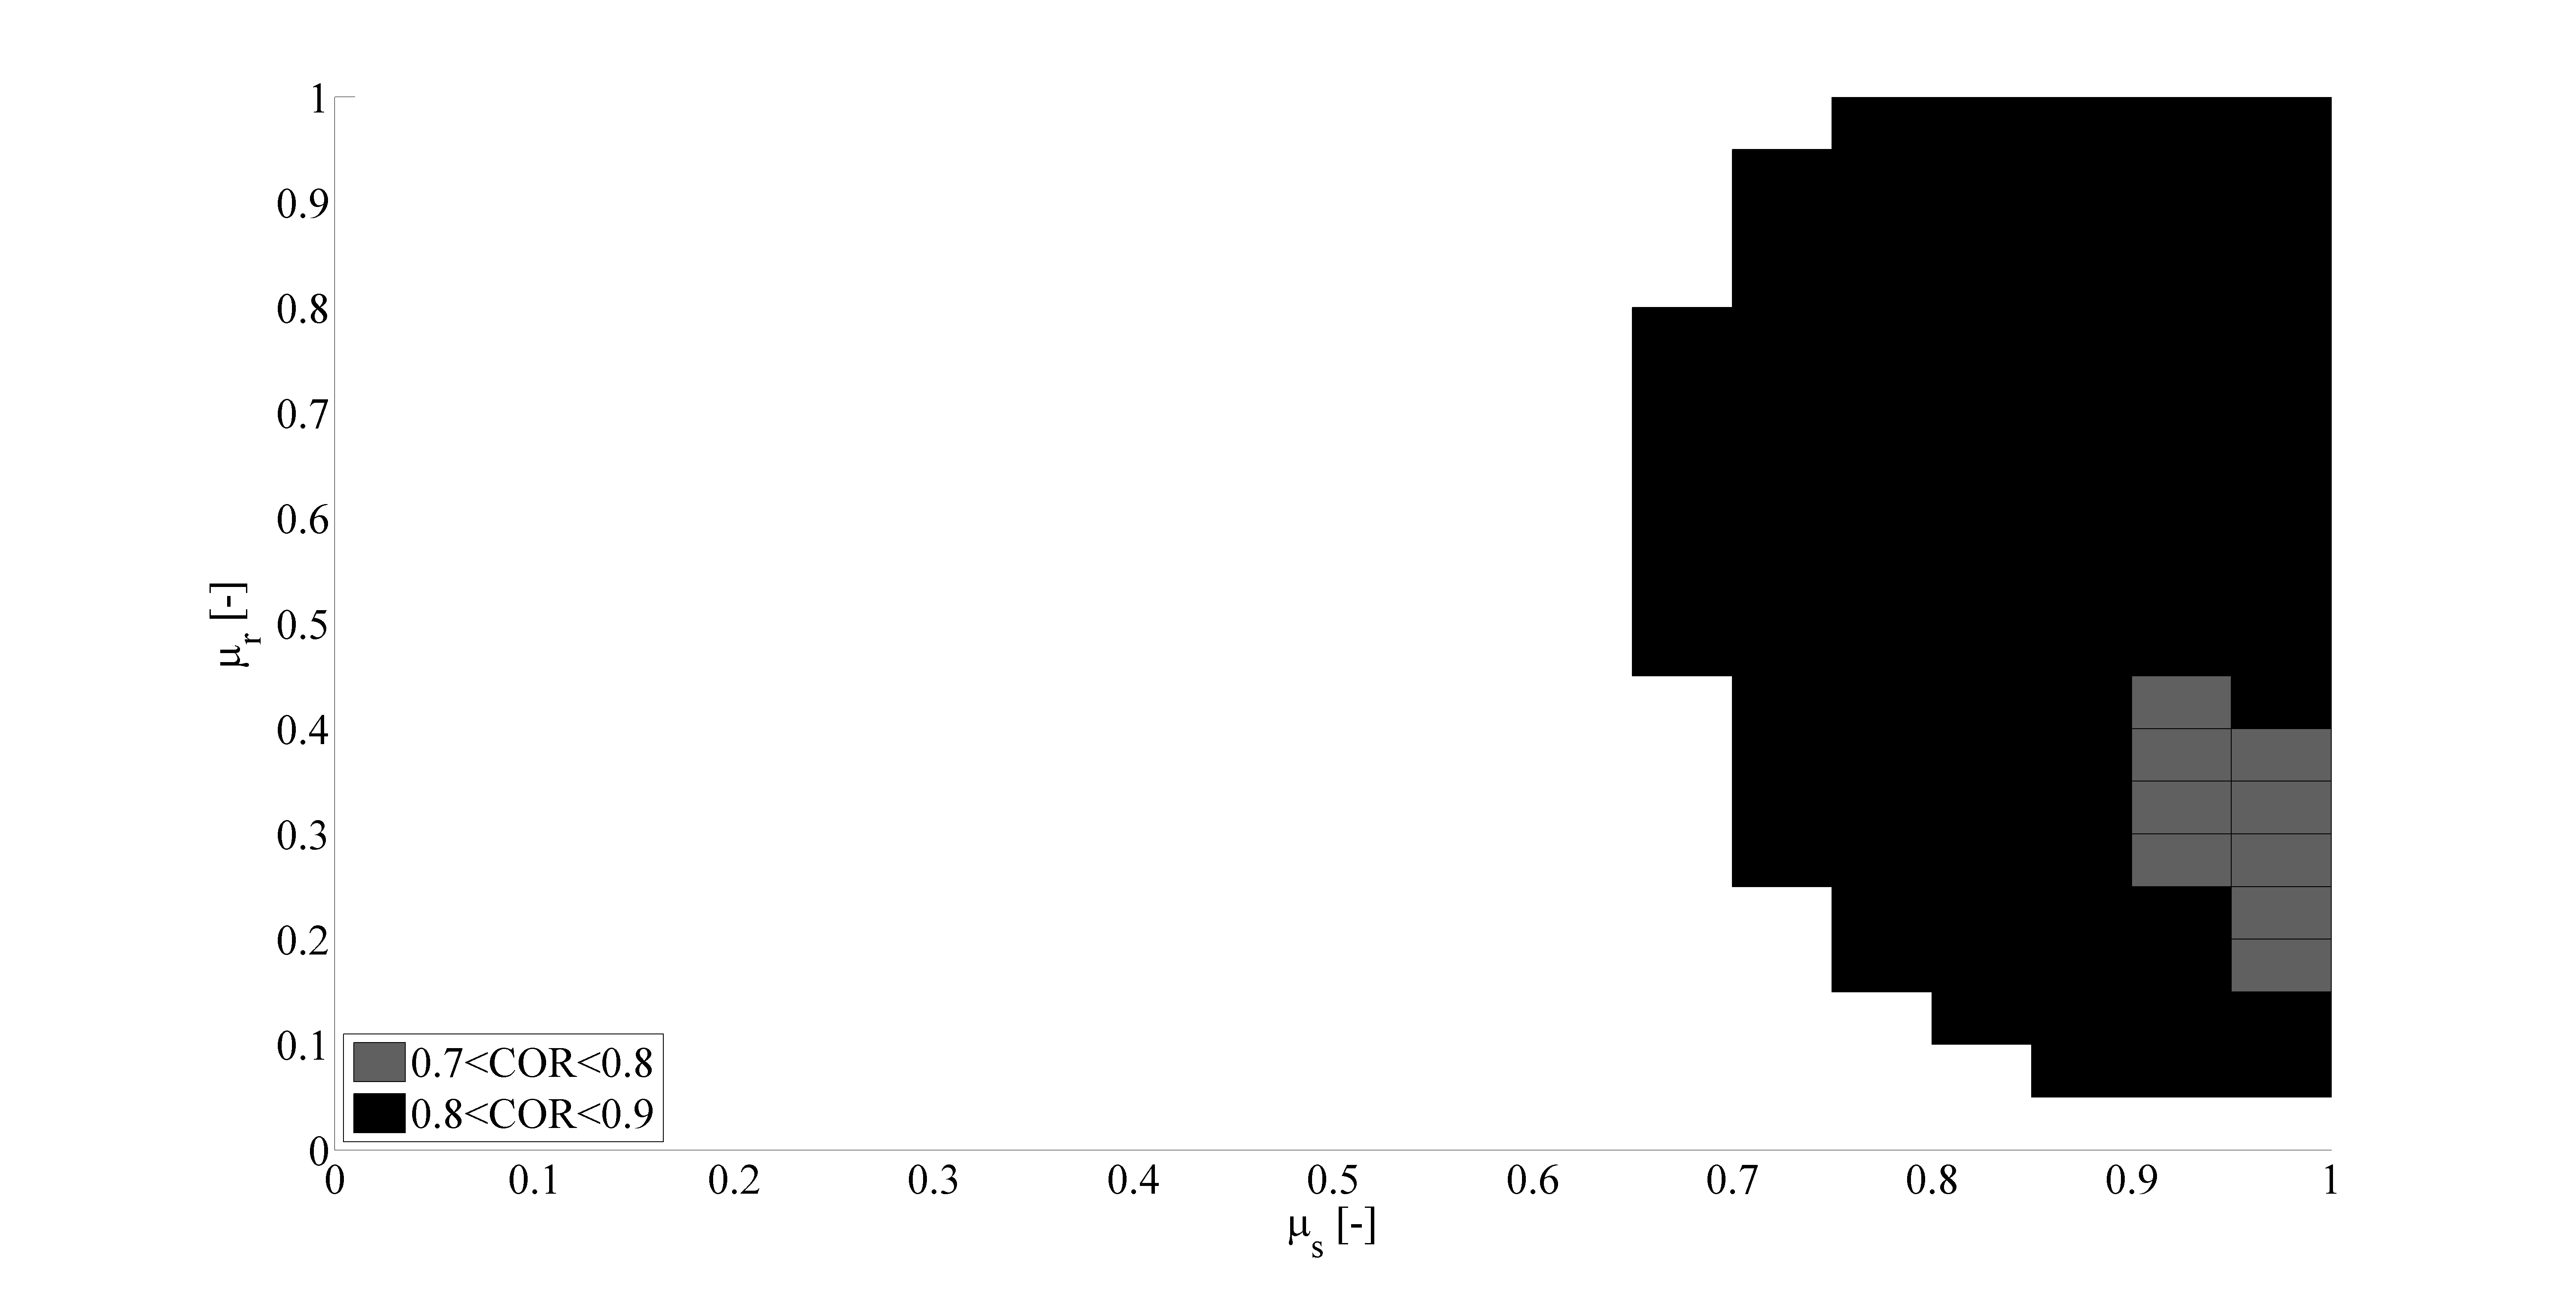
\includegraphics[width=.48\columnwidth]{images/030cloudpirker12schulze10070}
	  \label{fig:030cloudpirker12schulze10070}
  }
  \\
  \caption{Density plot comparison of SCT results.}
  \label{fig:080sctdensityplots}
\end{figure}
\begin{figure}[htbp]
\centering 
  \subfloat[Parameter space plot, $AoR_{exp} = 38.85 ^\circ$.]{
	  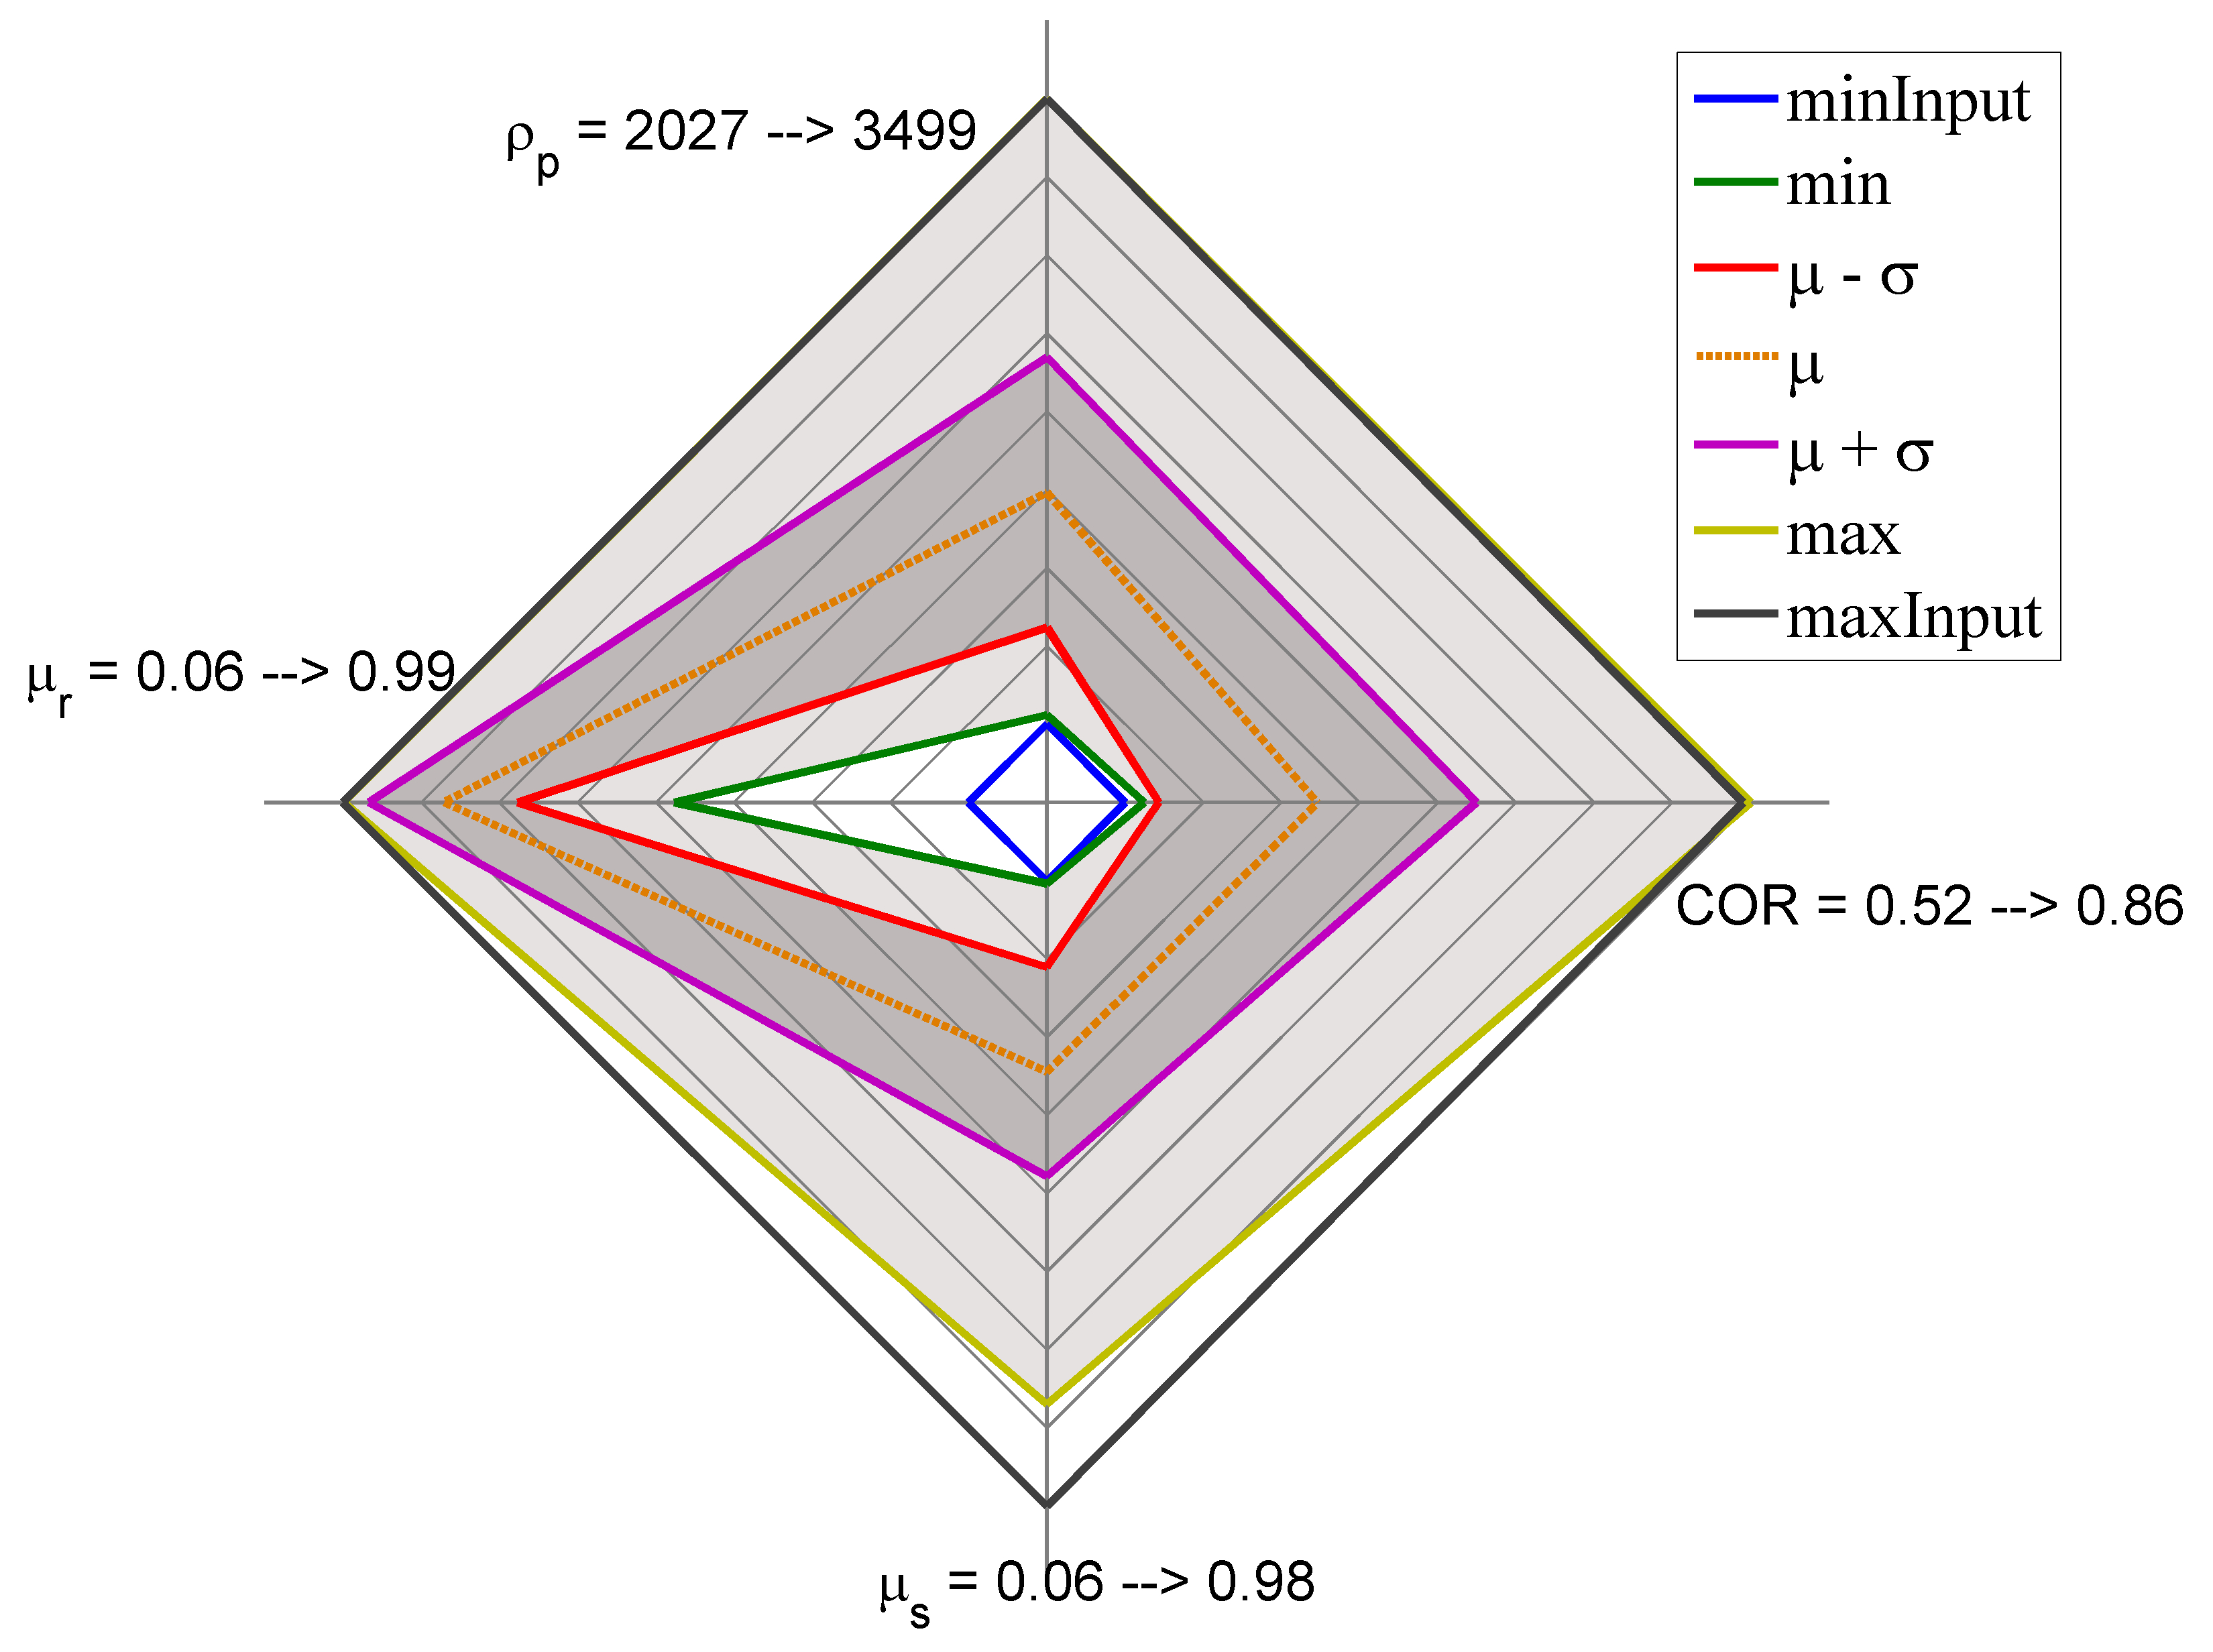
\includegraphics[width=.40\columnwidth]{images/031radarpirker1aor}
	  \label{fig:031radarpirker1aor}
  }
  \quad
    \subfloat[Box plot, $AoR_{exp} = 38.85 ^\circ$.]{
	  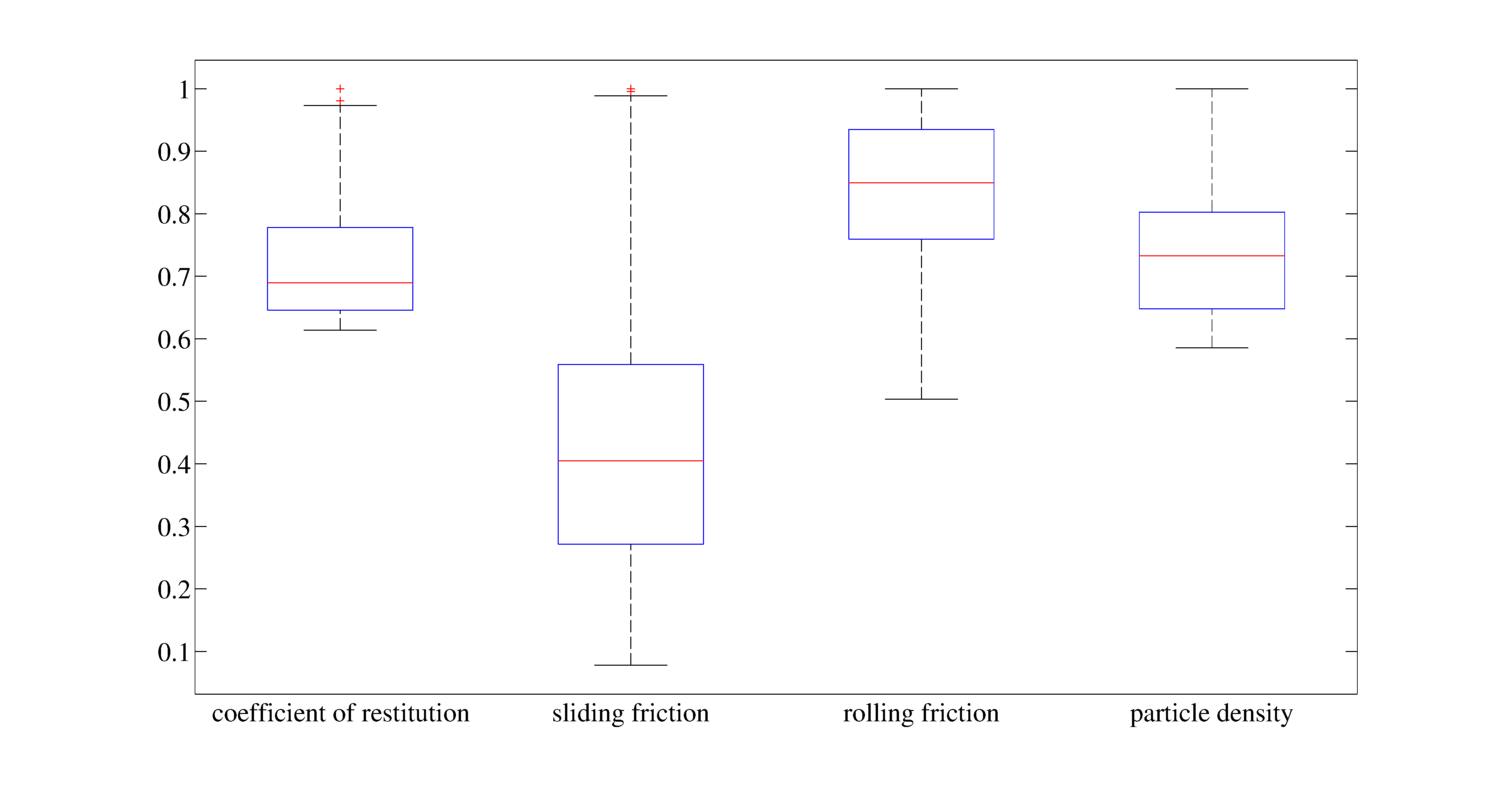
\includegraphics[width=.40\columnwidth]{images/076aorboxplot}
	  \label{fig:076aorboxplot}
  }
  \\
  \subfloat[Parameter space plot, $AoR_{exp} = 38.85 
        ^\circ$ \& $SSC$: $\sigma_n=10070$ Pa.]{
	  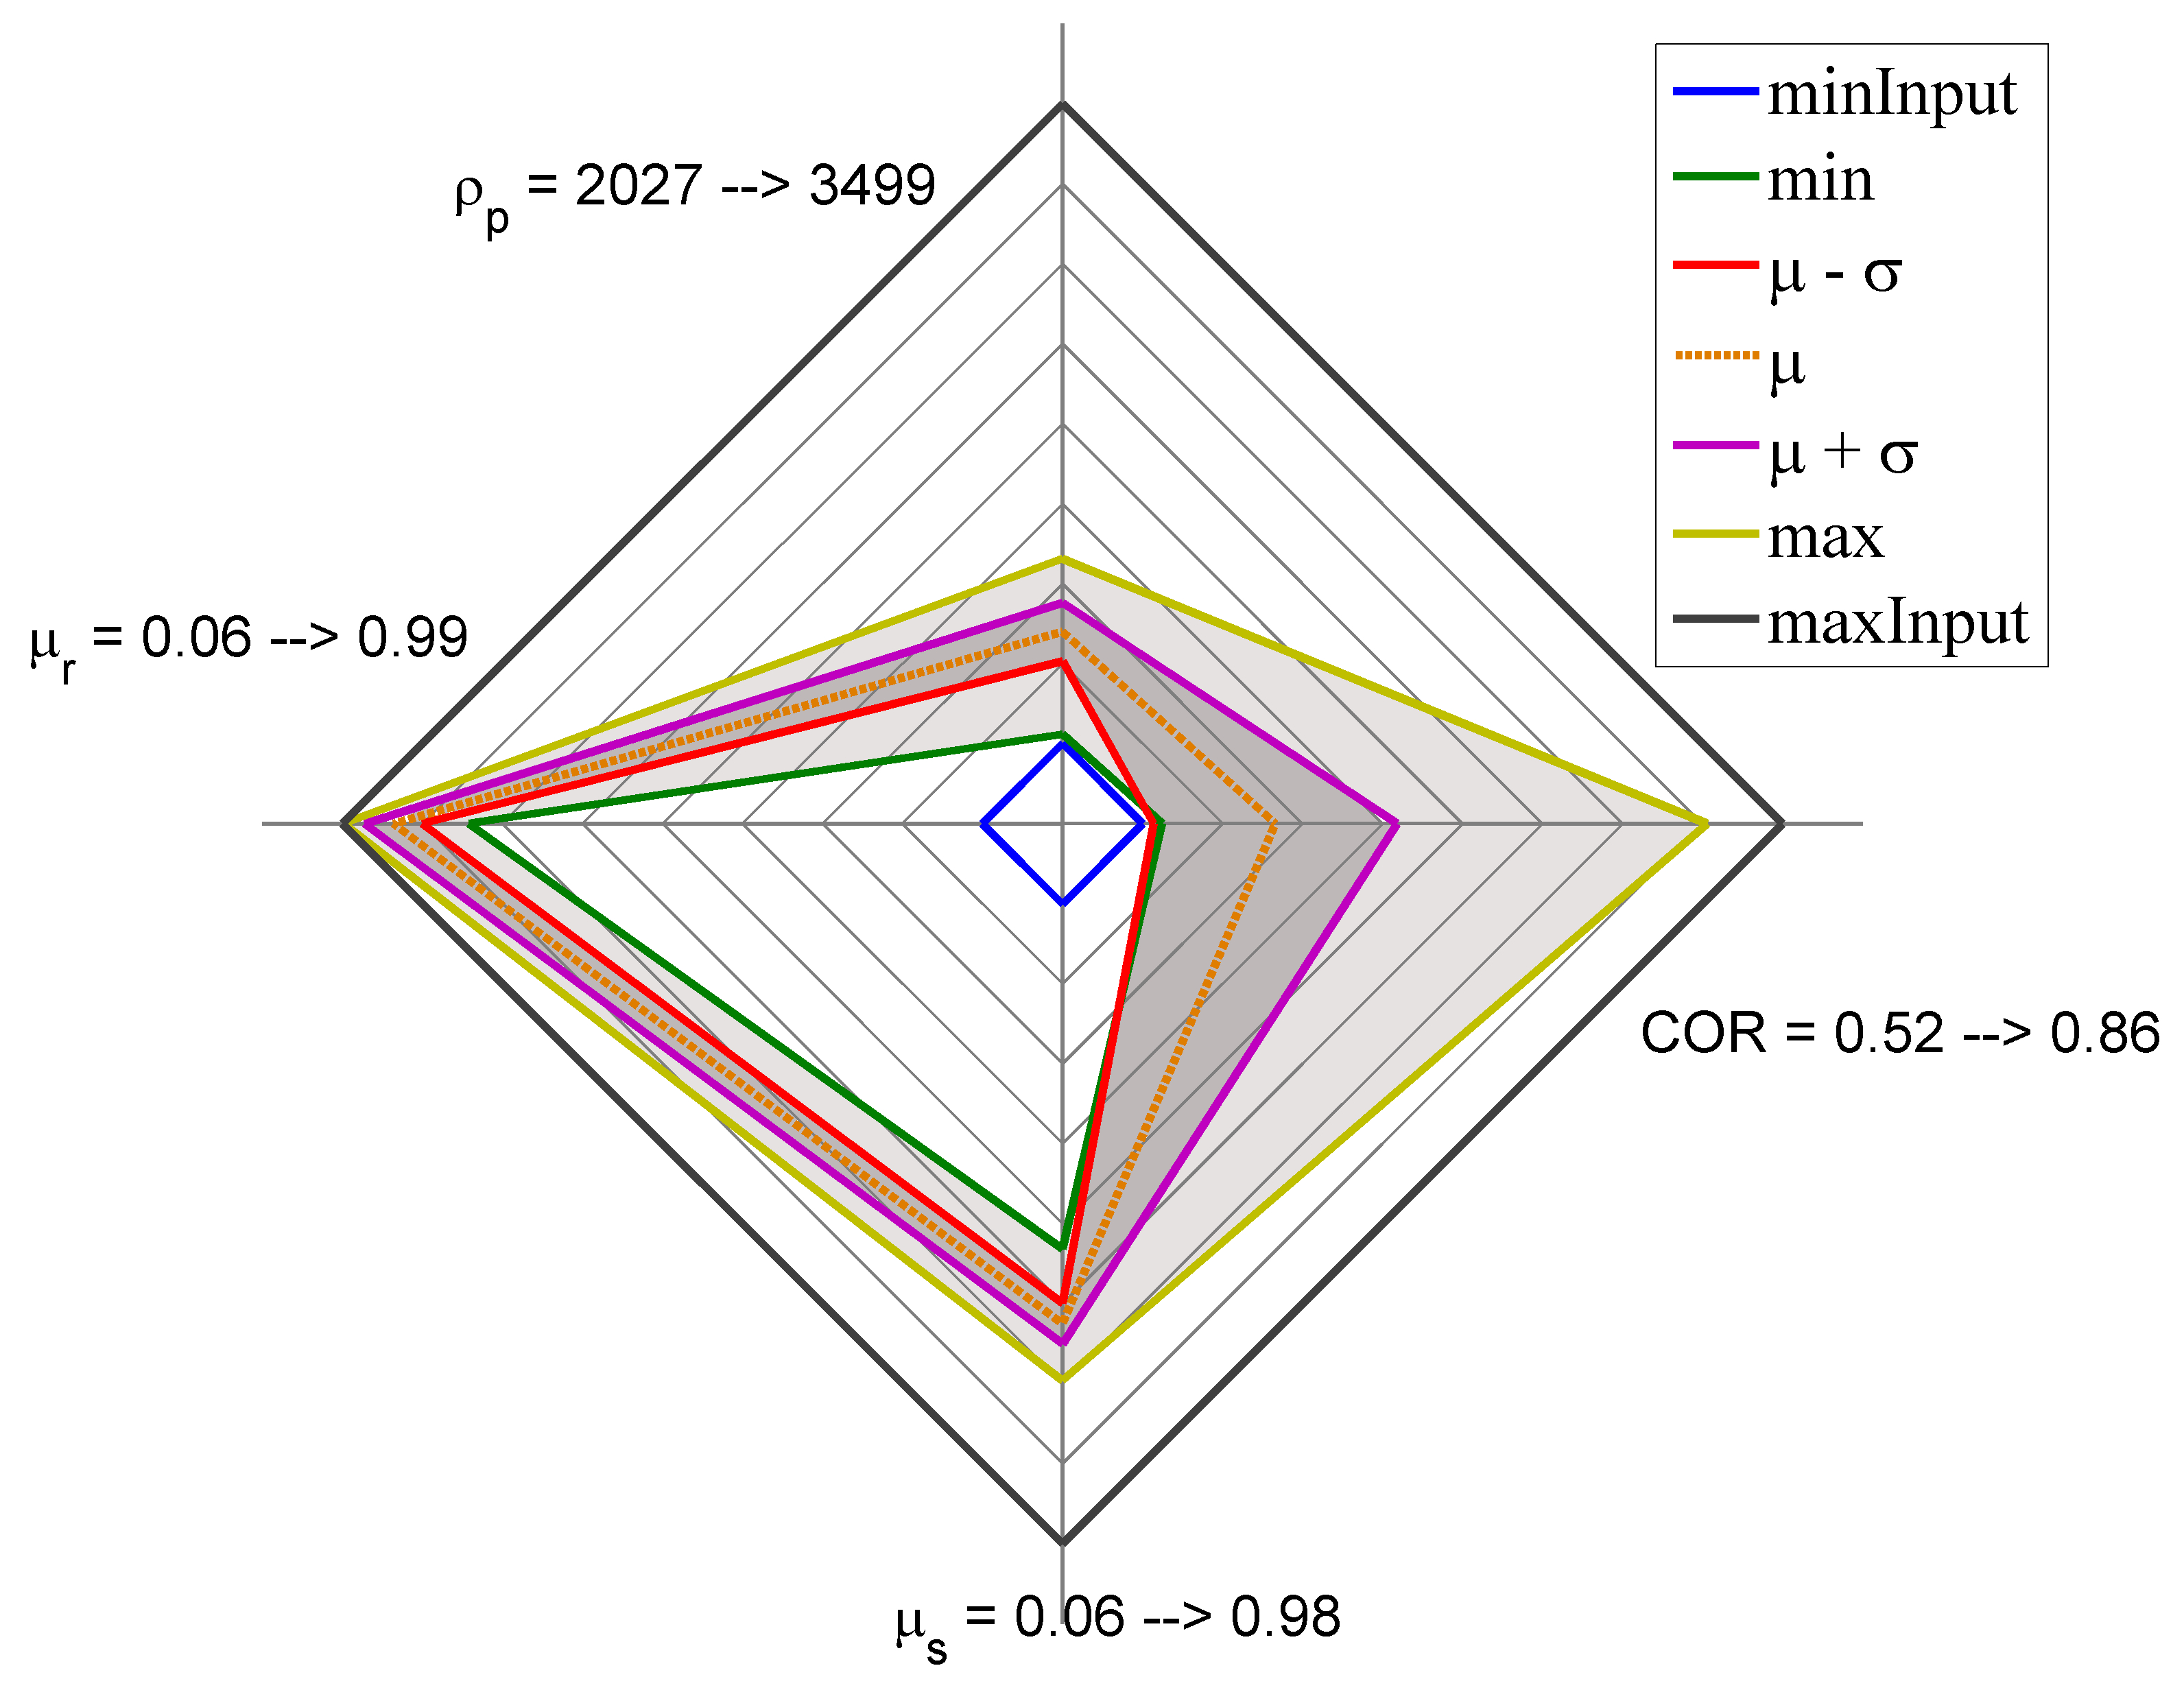
\includegraphics[width=.40\columnwidth]{images/033radarpirker1schulze10070aor}
	  \label{fig:033radarpirker1schulze10070aor}
  }
  \quad
    \subfloat[Box plot, $AoR_{exp} = 38.85
        ^\circ$ \& $SSC$: $\sigma_n=10070$ Pa.]{
	  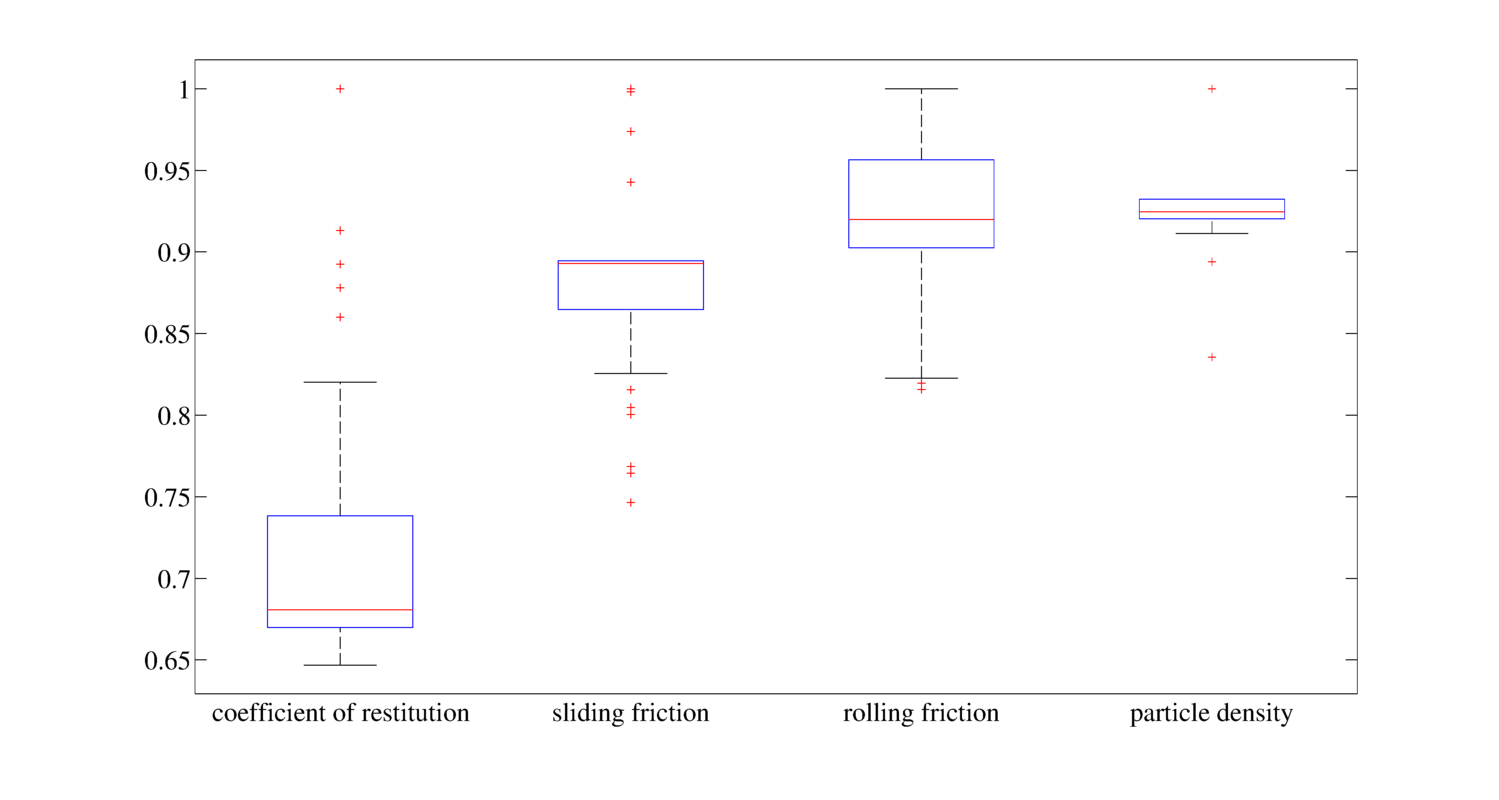
\includegraphics[width=.40\columnwidth]{images/078mergeboxplot}
	  \label{fig:078mergeboxplot}  }
  \\
  \caption{AoR and merge parameter space plots.}
  \label{fig:081aorandmergeparameterspaceplots}
\end{figure}



%************************************************
%************************************************

\section{Influence of poly-dispersity}
\label{sec:polydispersity}
%************************************************

\info{Some examples of the new images: relationship between the standard
deviation of the radius and the shape of the tile plot.}

\improvement{table similar to \ref{tab:12DEMRandominputvalues} here}
\wrong{separate all images into single with captions}
\change{add box plots?}

Fig. \ref{fig:082ironore0315}\\
\begin{figure}[!htb]
\centering
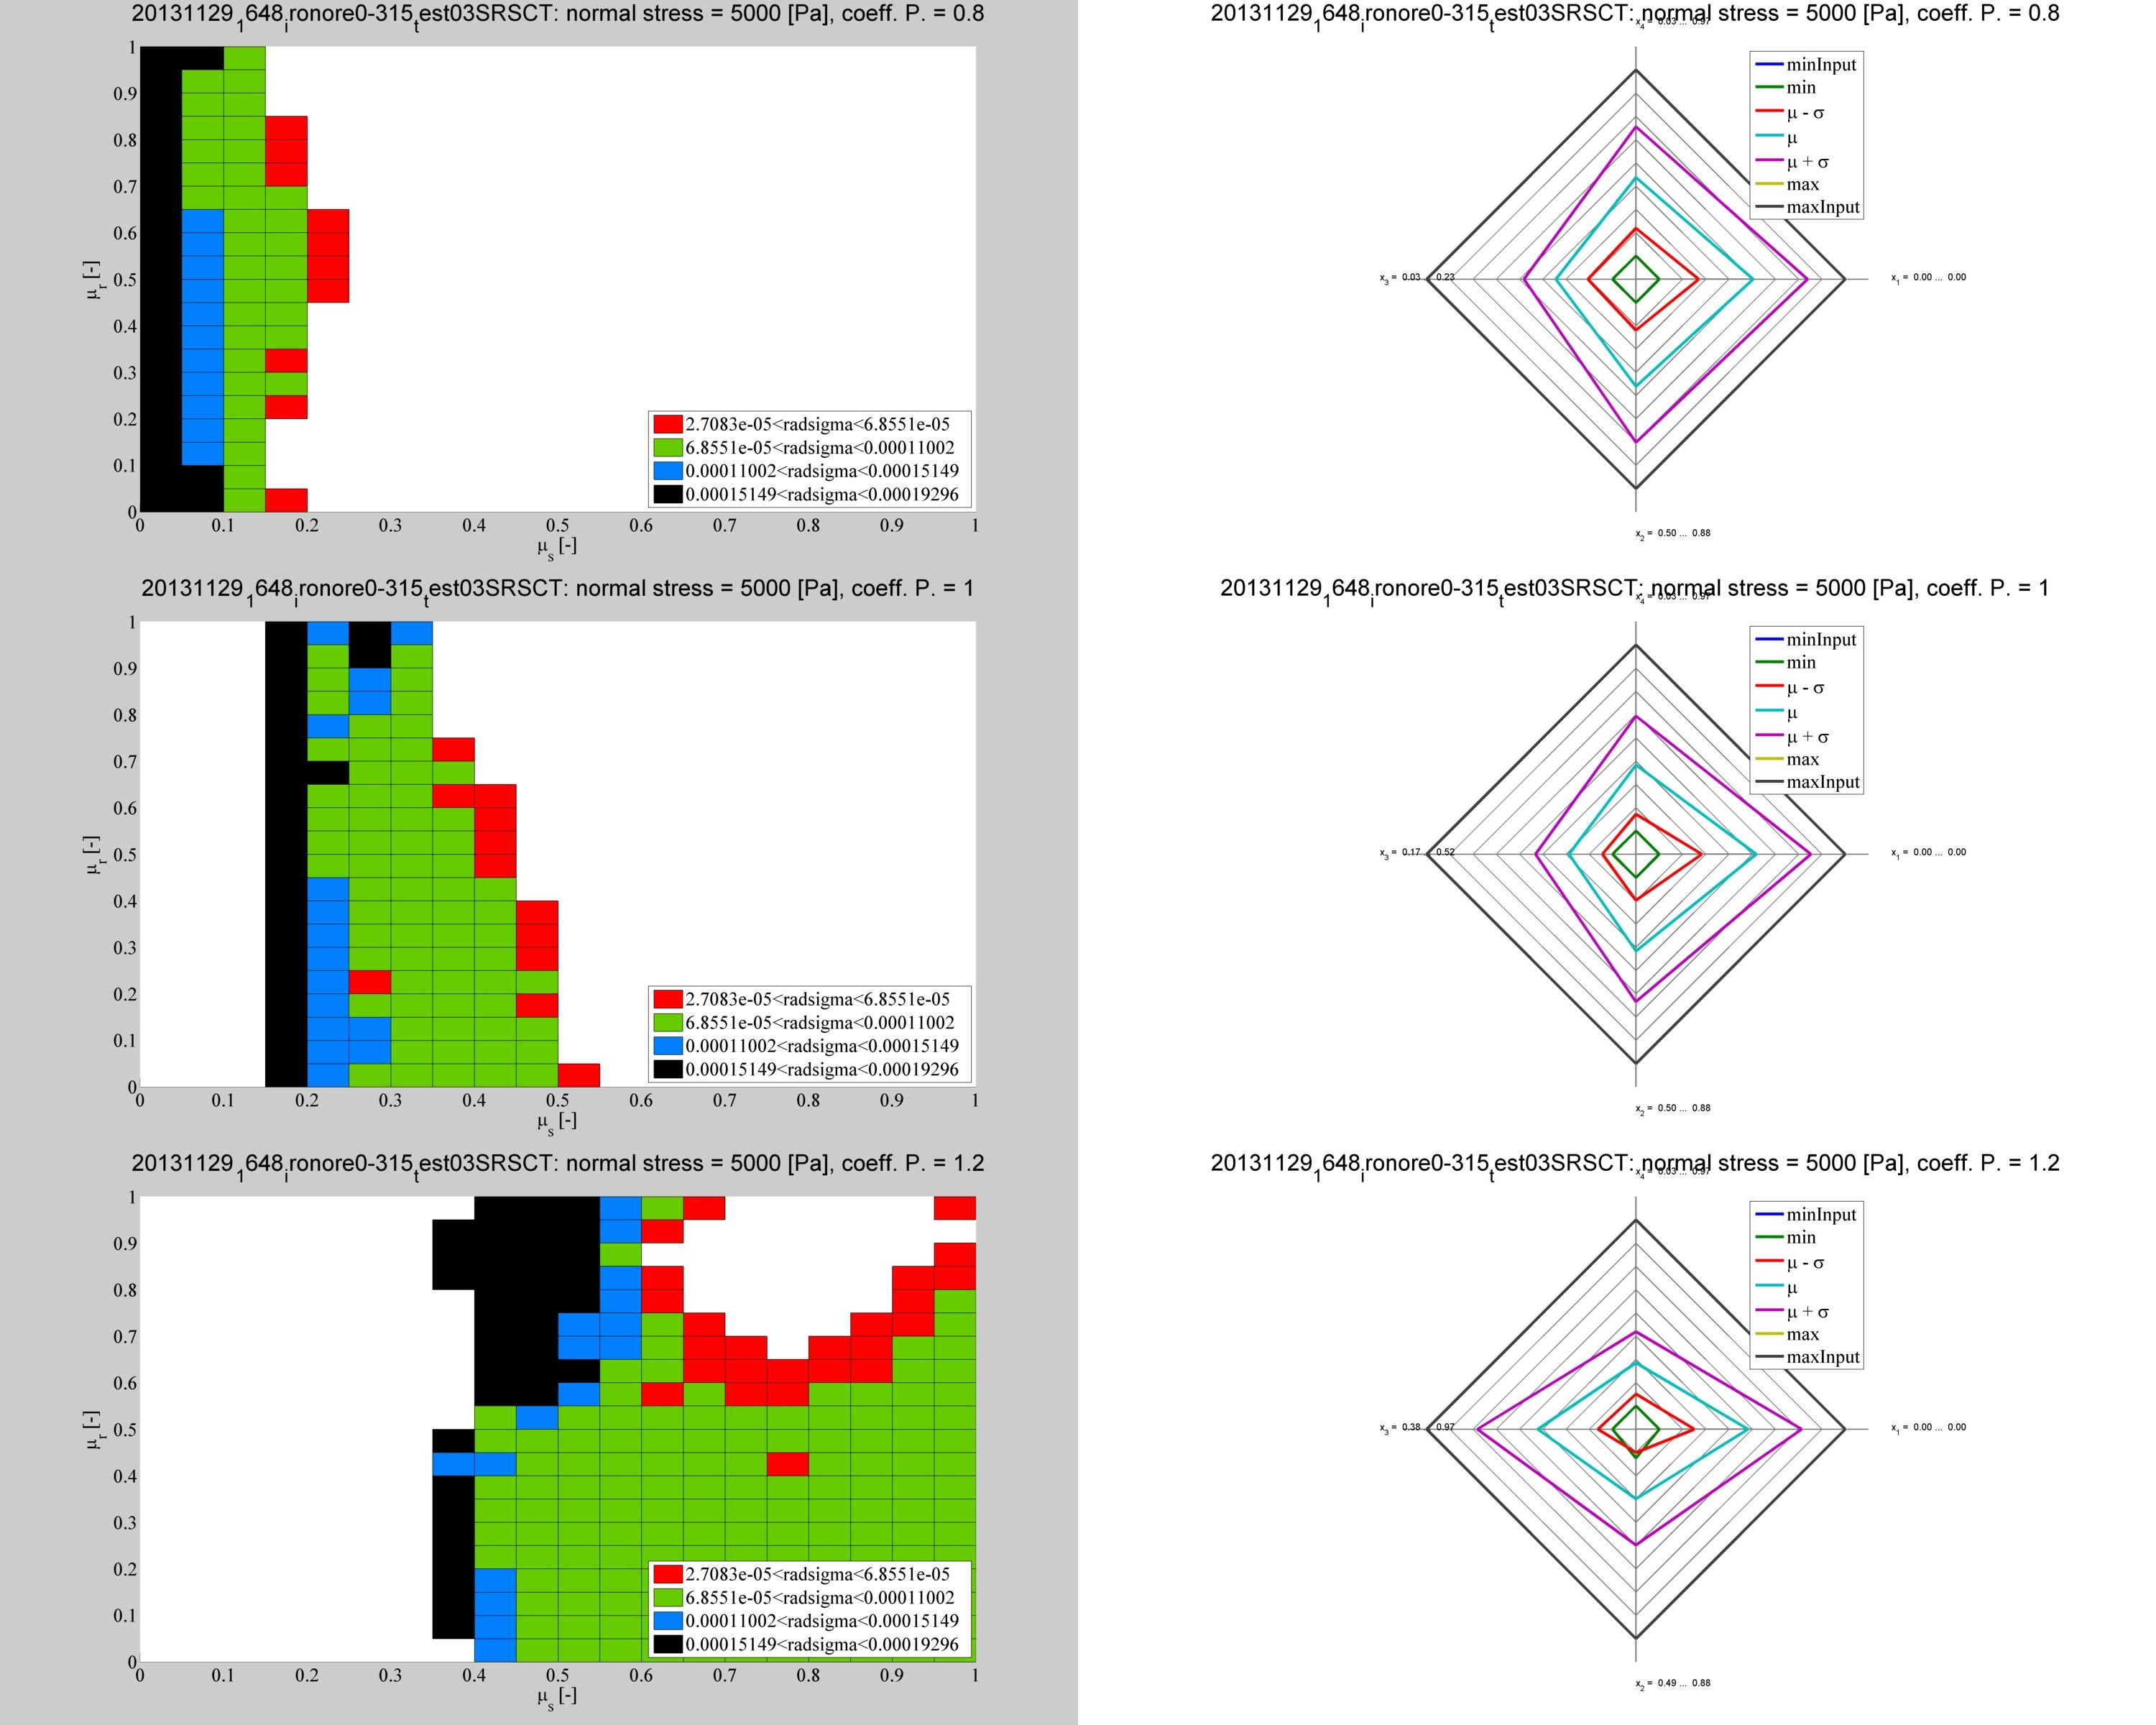
\includegraphics[width=.96\columnwidth]{images/082ironore0315}
\caption[Iron ore fine polidispersity evaluation]{Iron ore fine polidispersity evaluation.}
\label{fig:082ironore0315}
\end{figure}

Fig. \ref{fig:083ironore31510}\\
\begin{figure}[!htb]
\centering
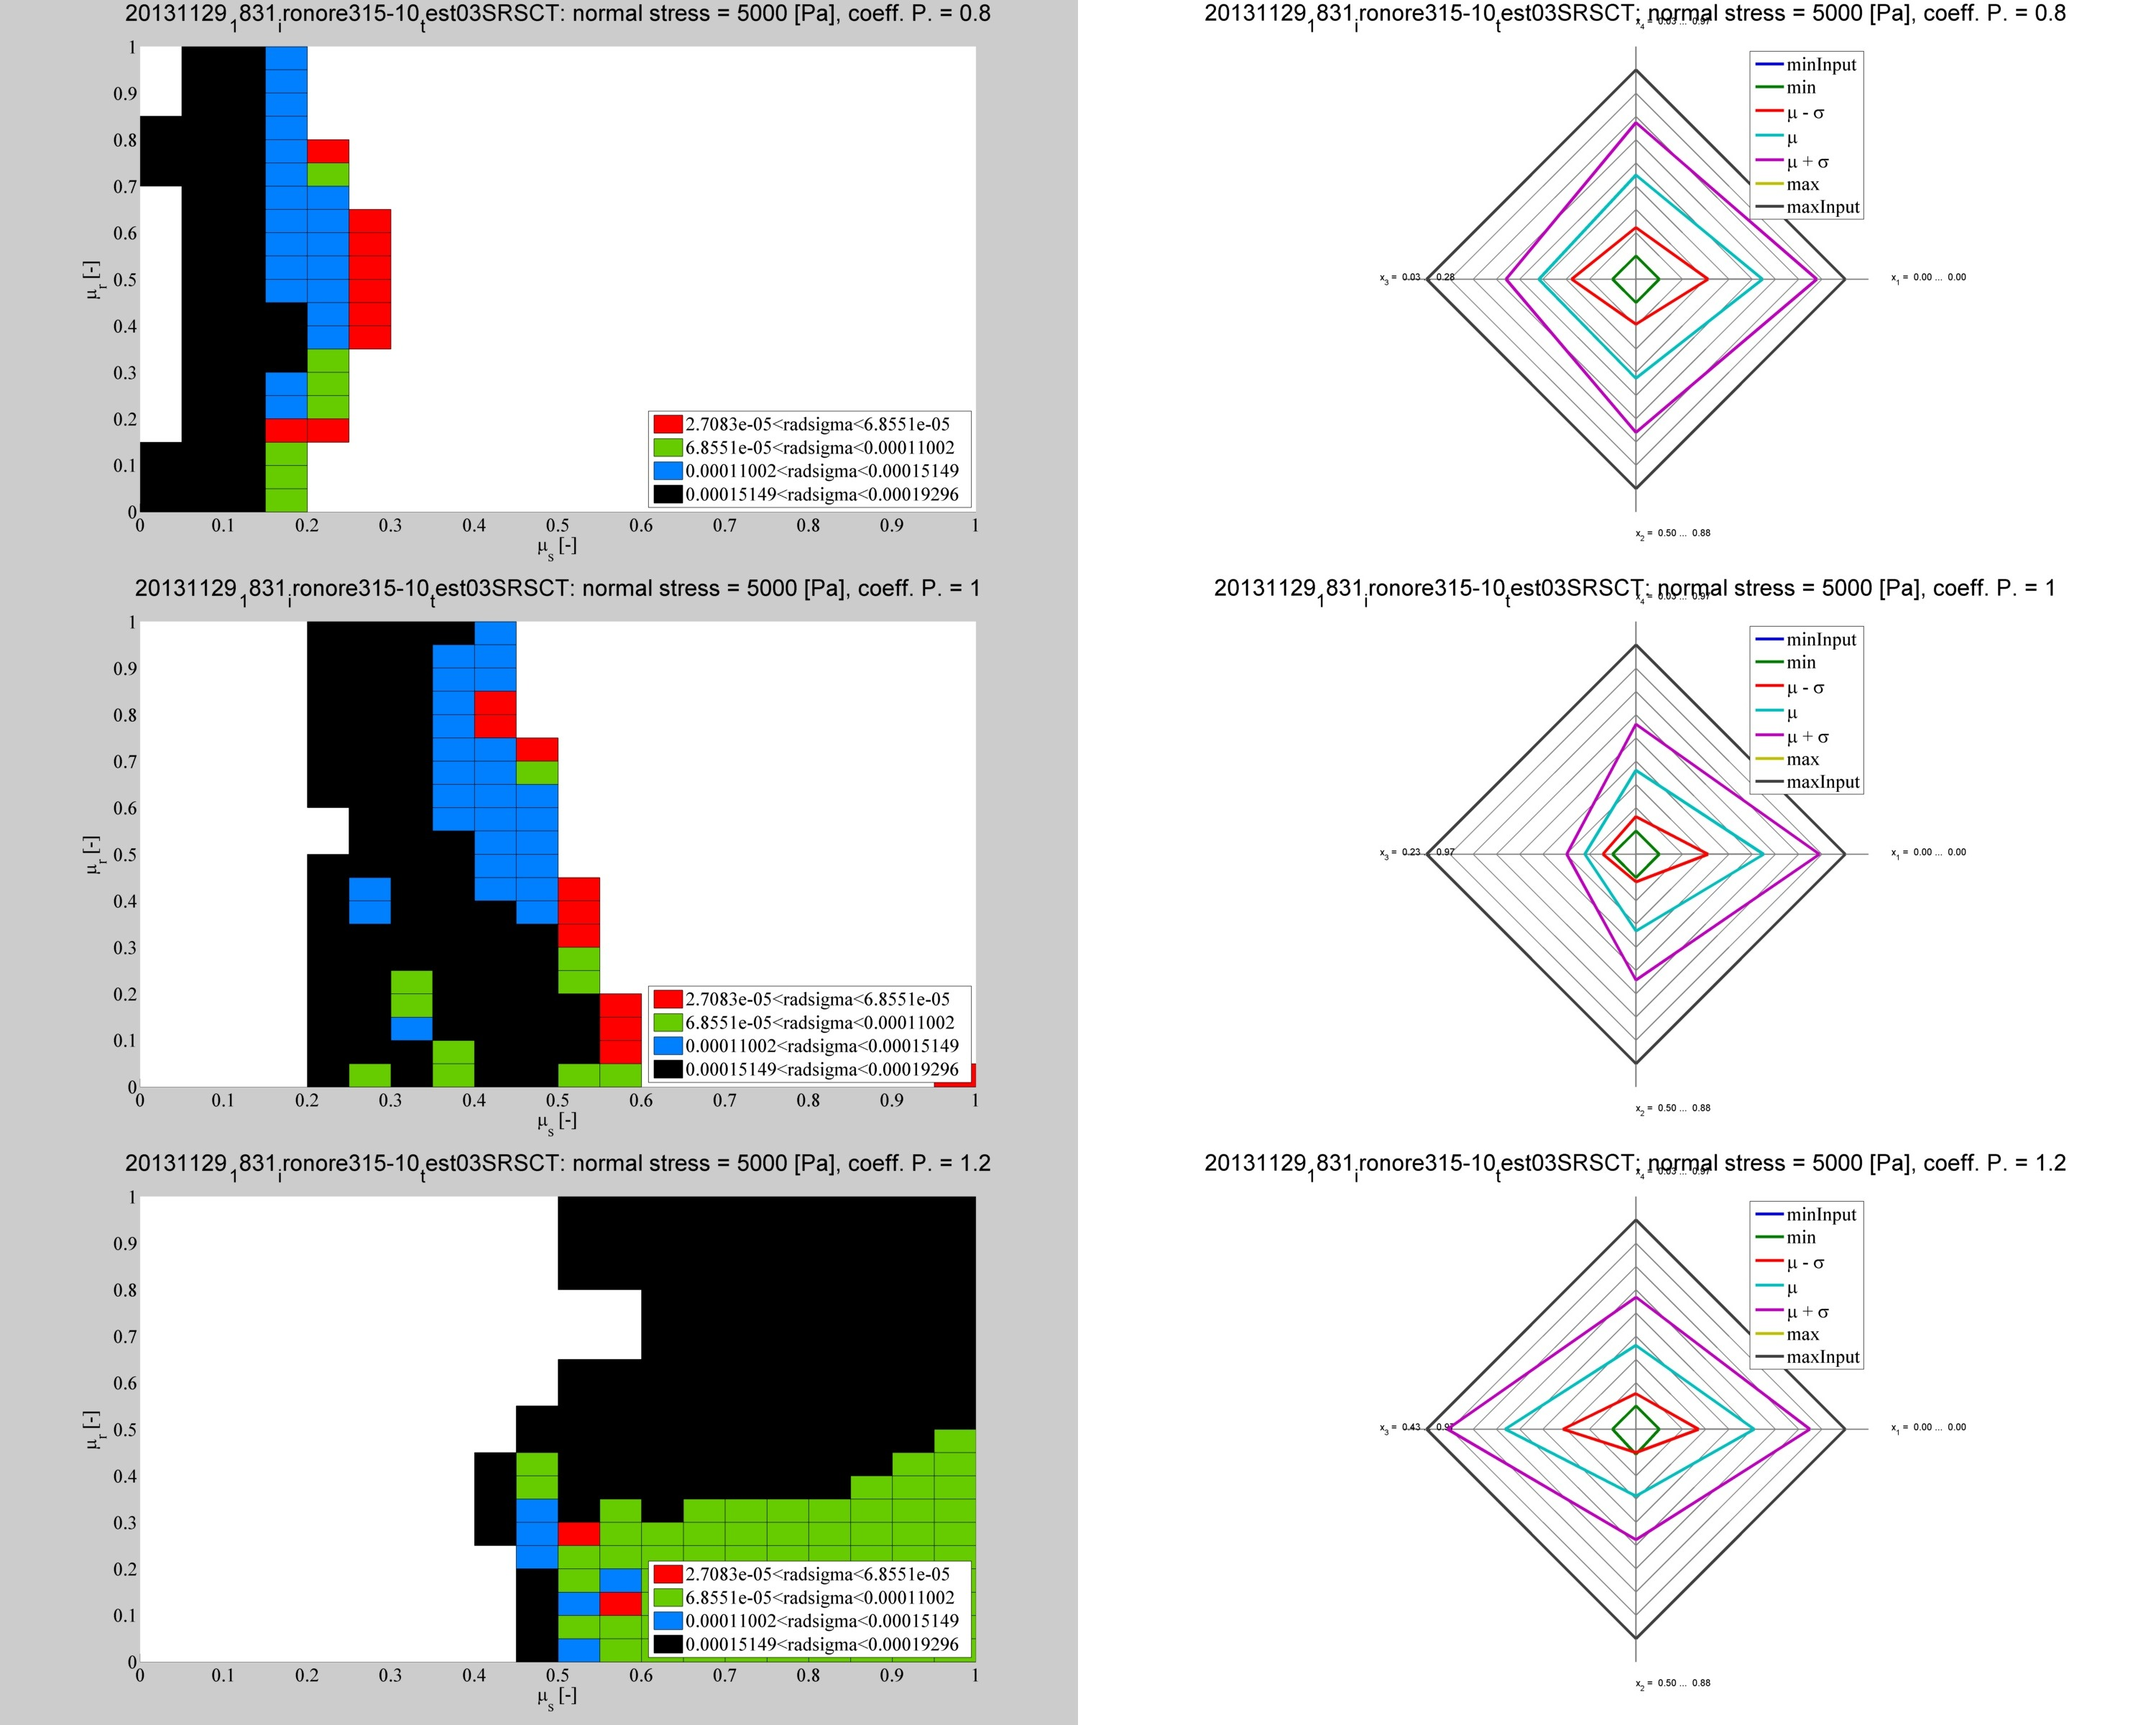
\includegraphics[width=.96\columnwidth]{images/083ironore31510}
\caption[Iron ore coarse polydispersity evaluation]{Iron ore coarse polydispersity
evaluation.}
\label{fig:083ironore31510}
\end{figure}

Fig. \ref{fig:084limestone0315}\\
\begin{figure}[!htb]
\centering
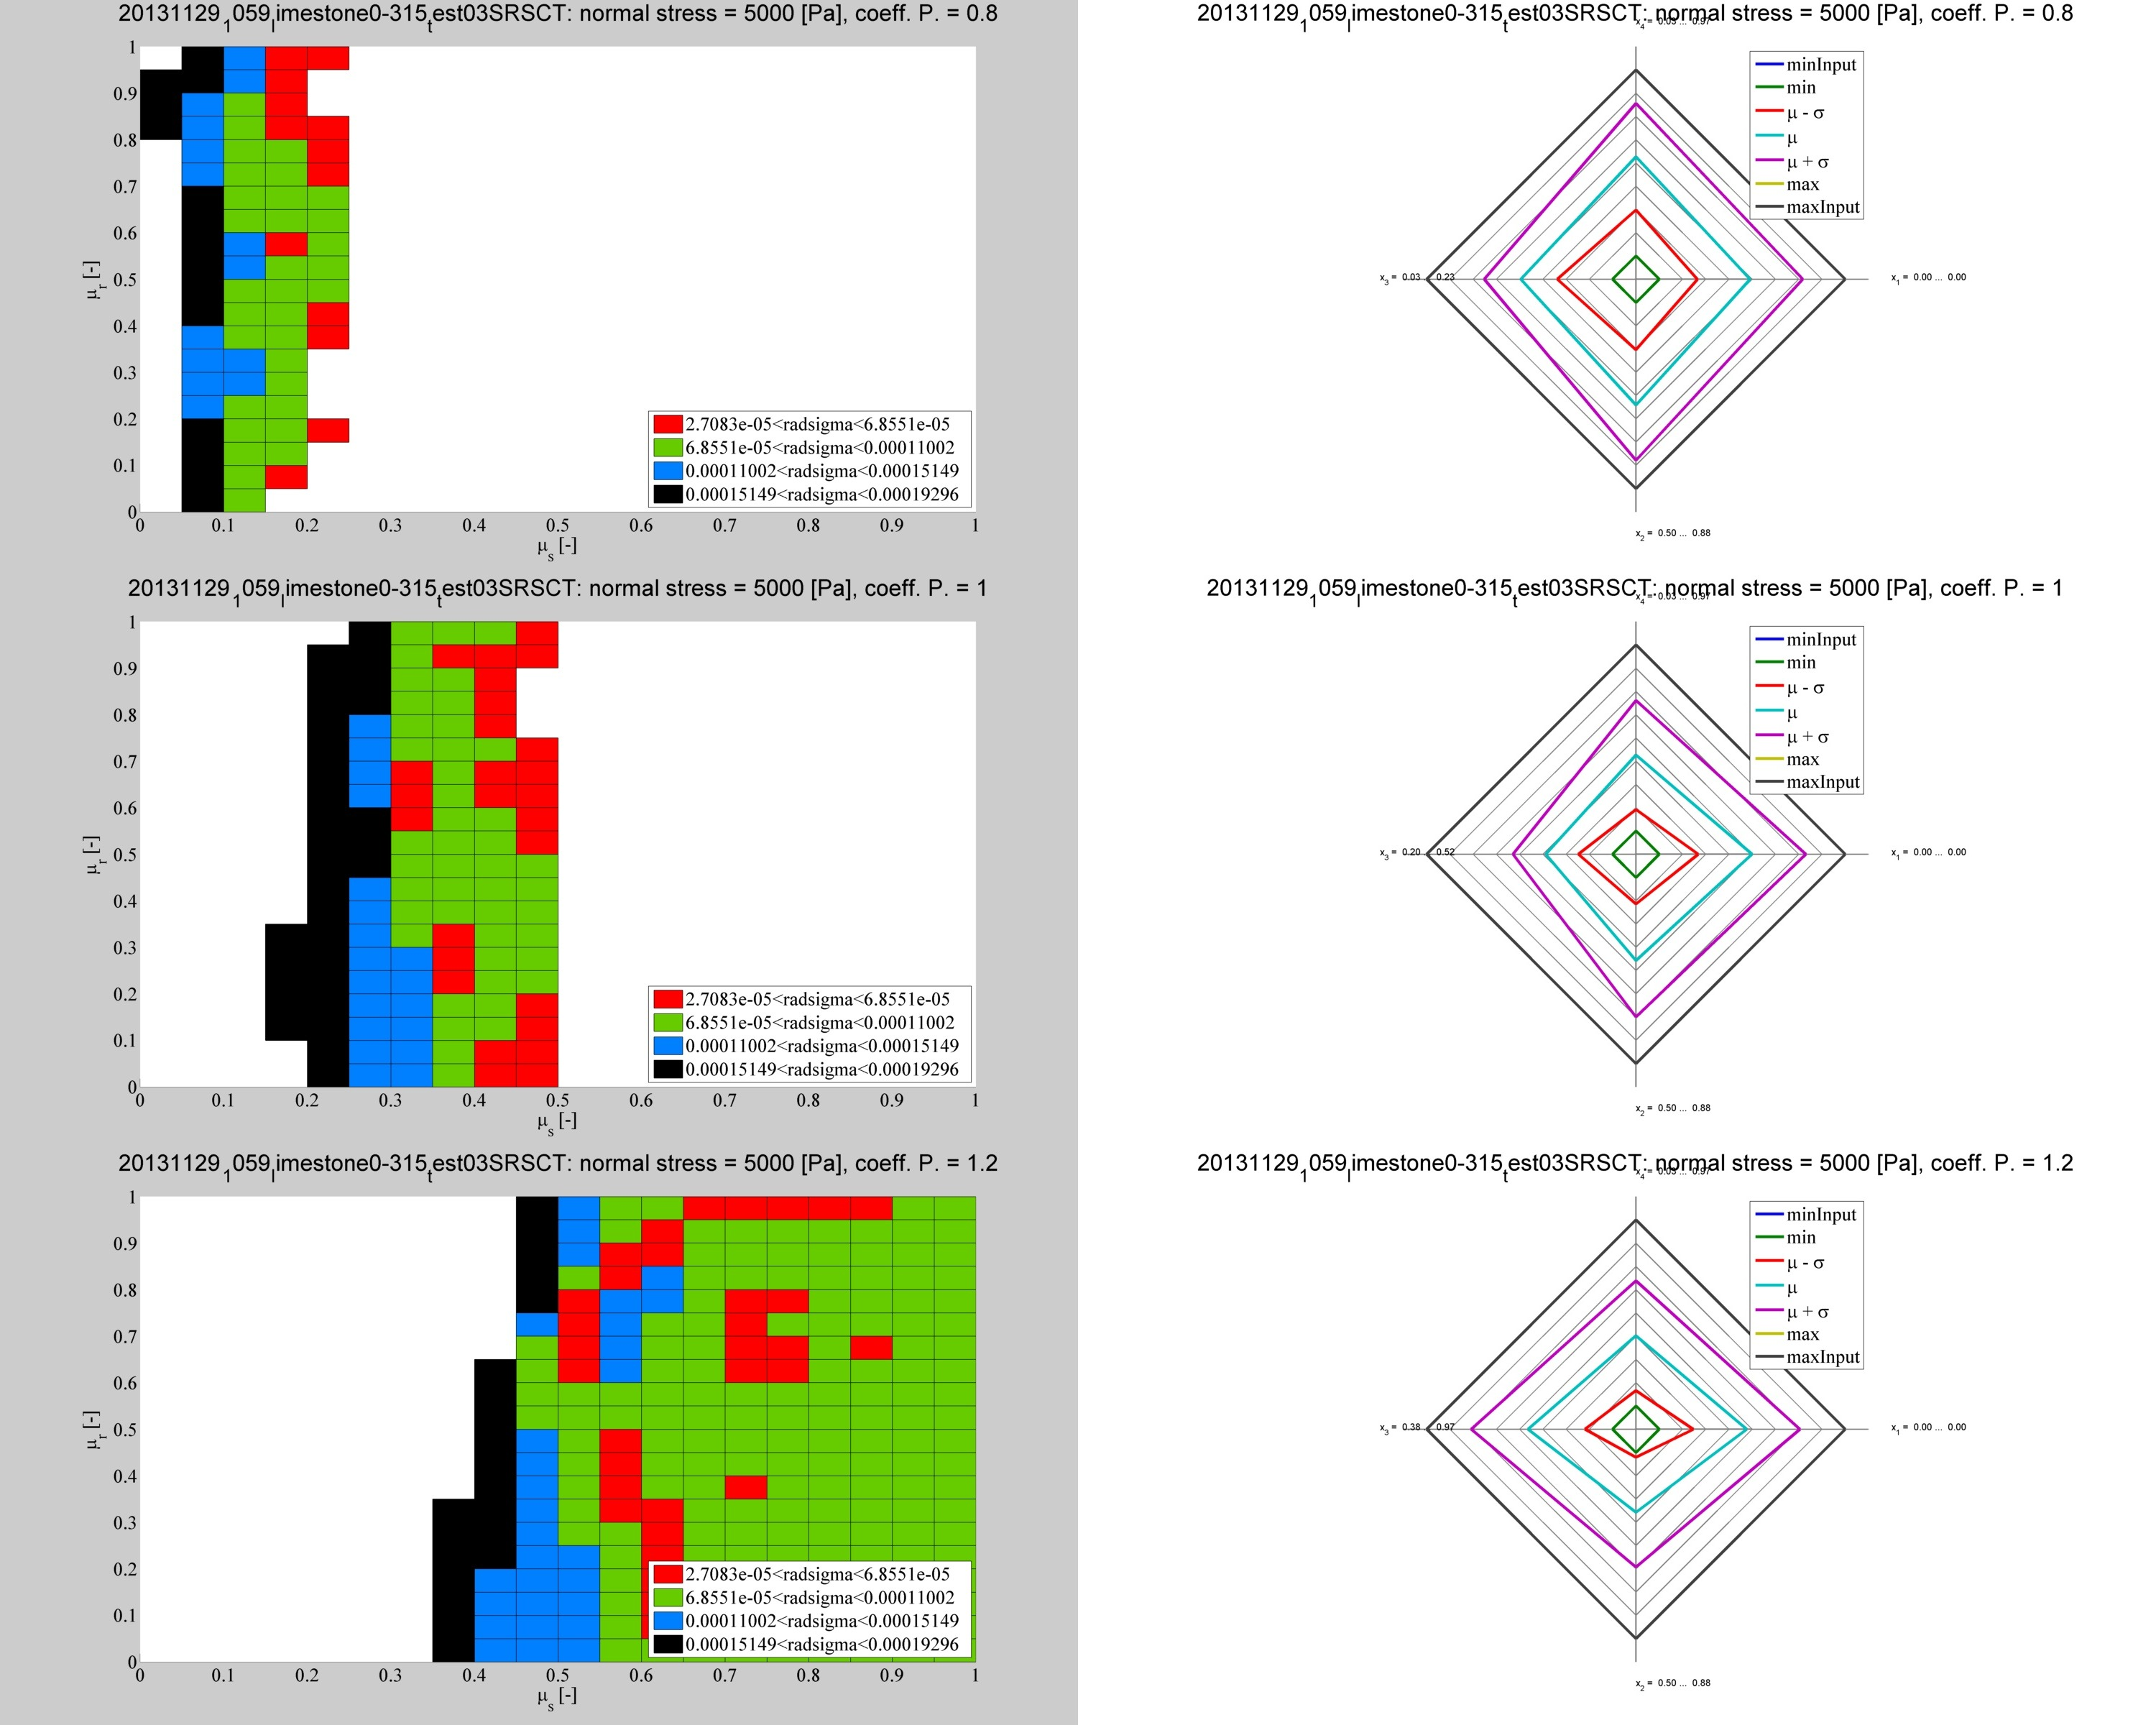
\includegraphics[width=.96\columnwidth]{images/084limestone0315}
\caption[Limestone fine polydispersity evaluation]{Limestone fine polydispersity evaluation.}
\label{fig:084limestone0315}
\end{figure}

Fig. \ref{fig:085limestone31510}\\
\begin{figure}[!htb]
\centering
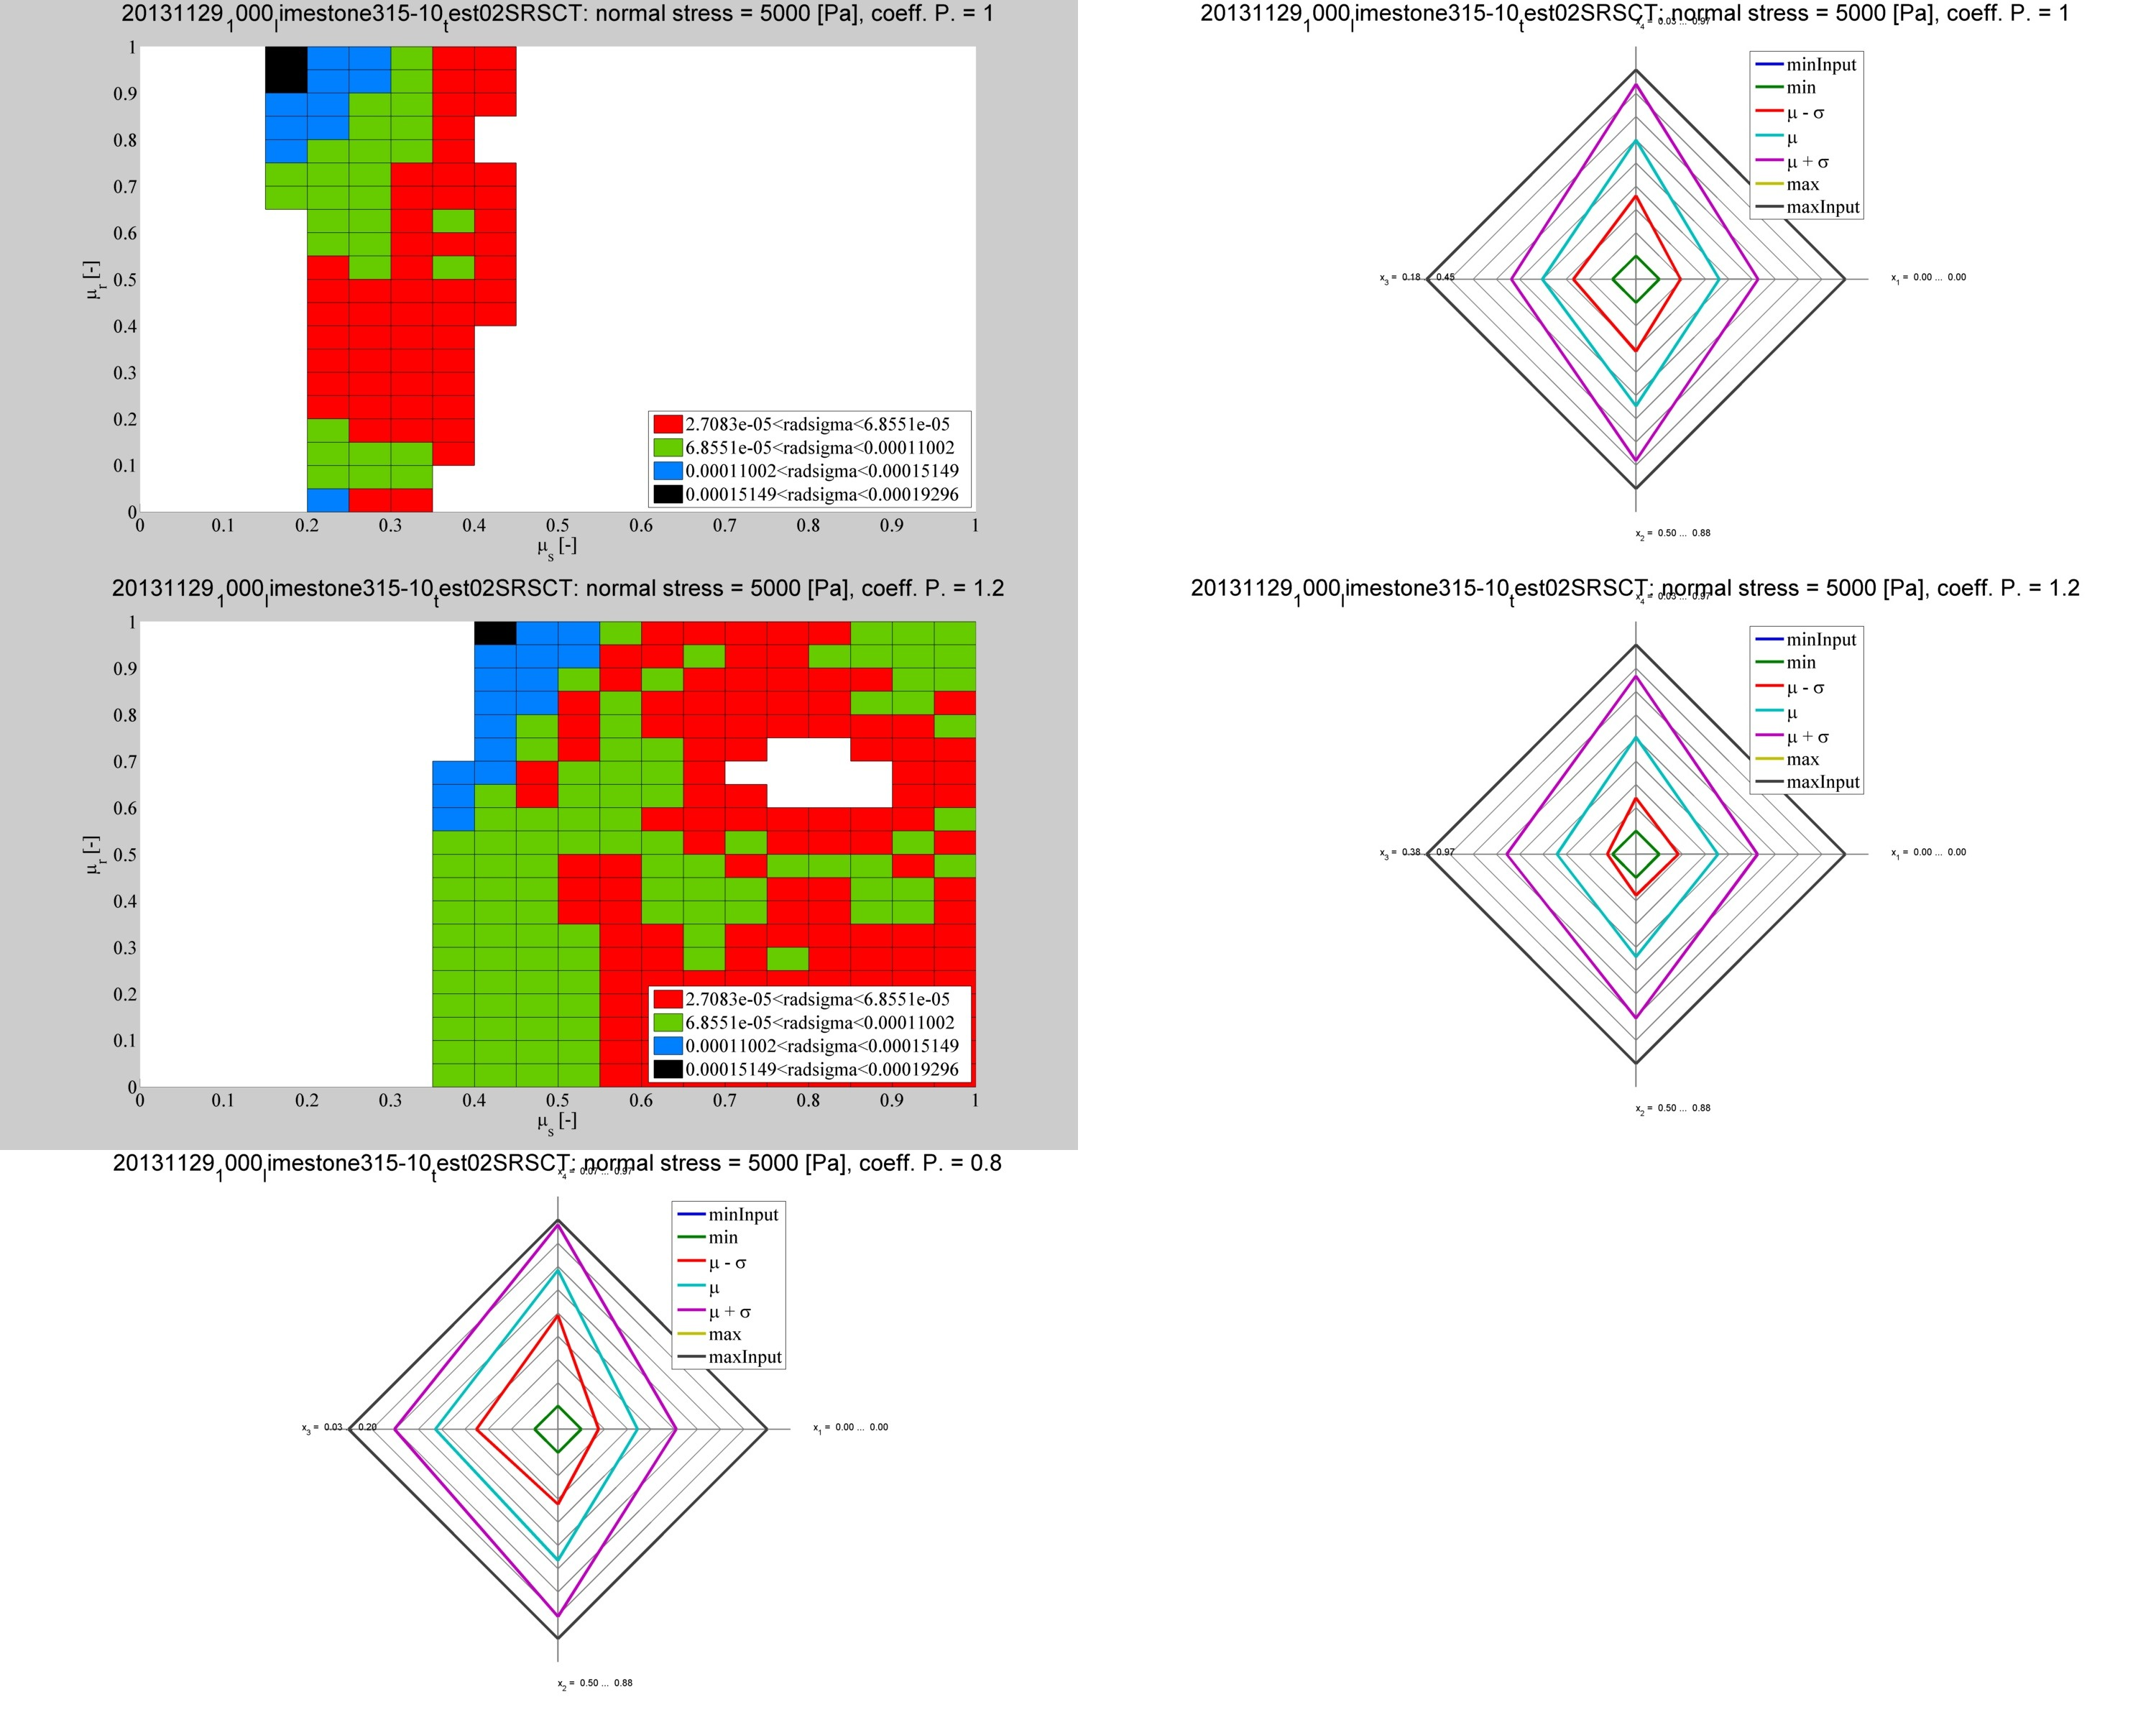
\includegraphics[width=.96\columnwidth]{images/085limestone31510}
\caption[Limestone coarse polydispersity evaluation]{Limestone coarse polydispersity
evaluation.}
\label{fig:085limestone31510}
\end{figure}

Fig. \ref{fig:086sinter0315}\\
\begin{figure}[!htb]
\centering
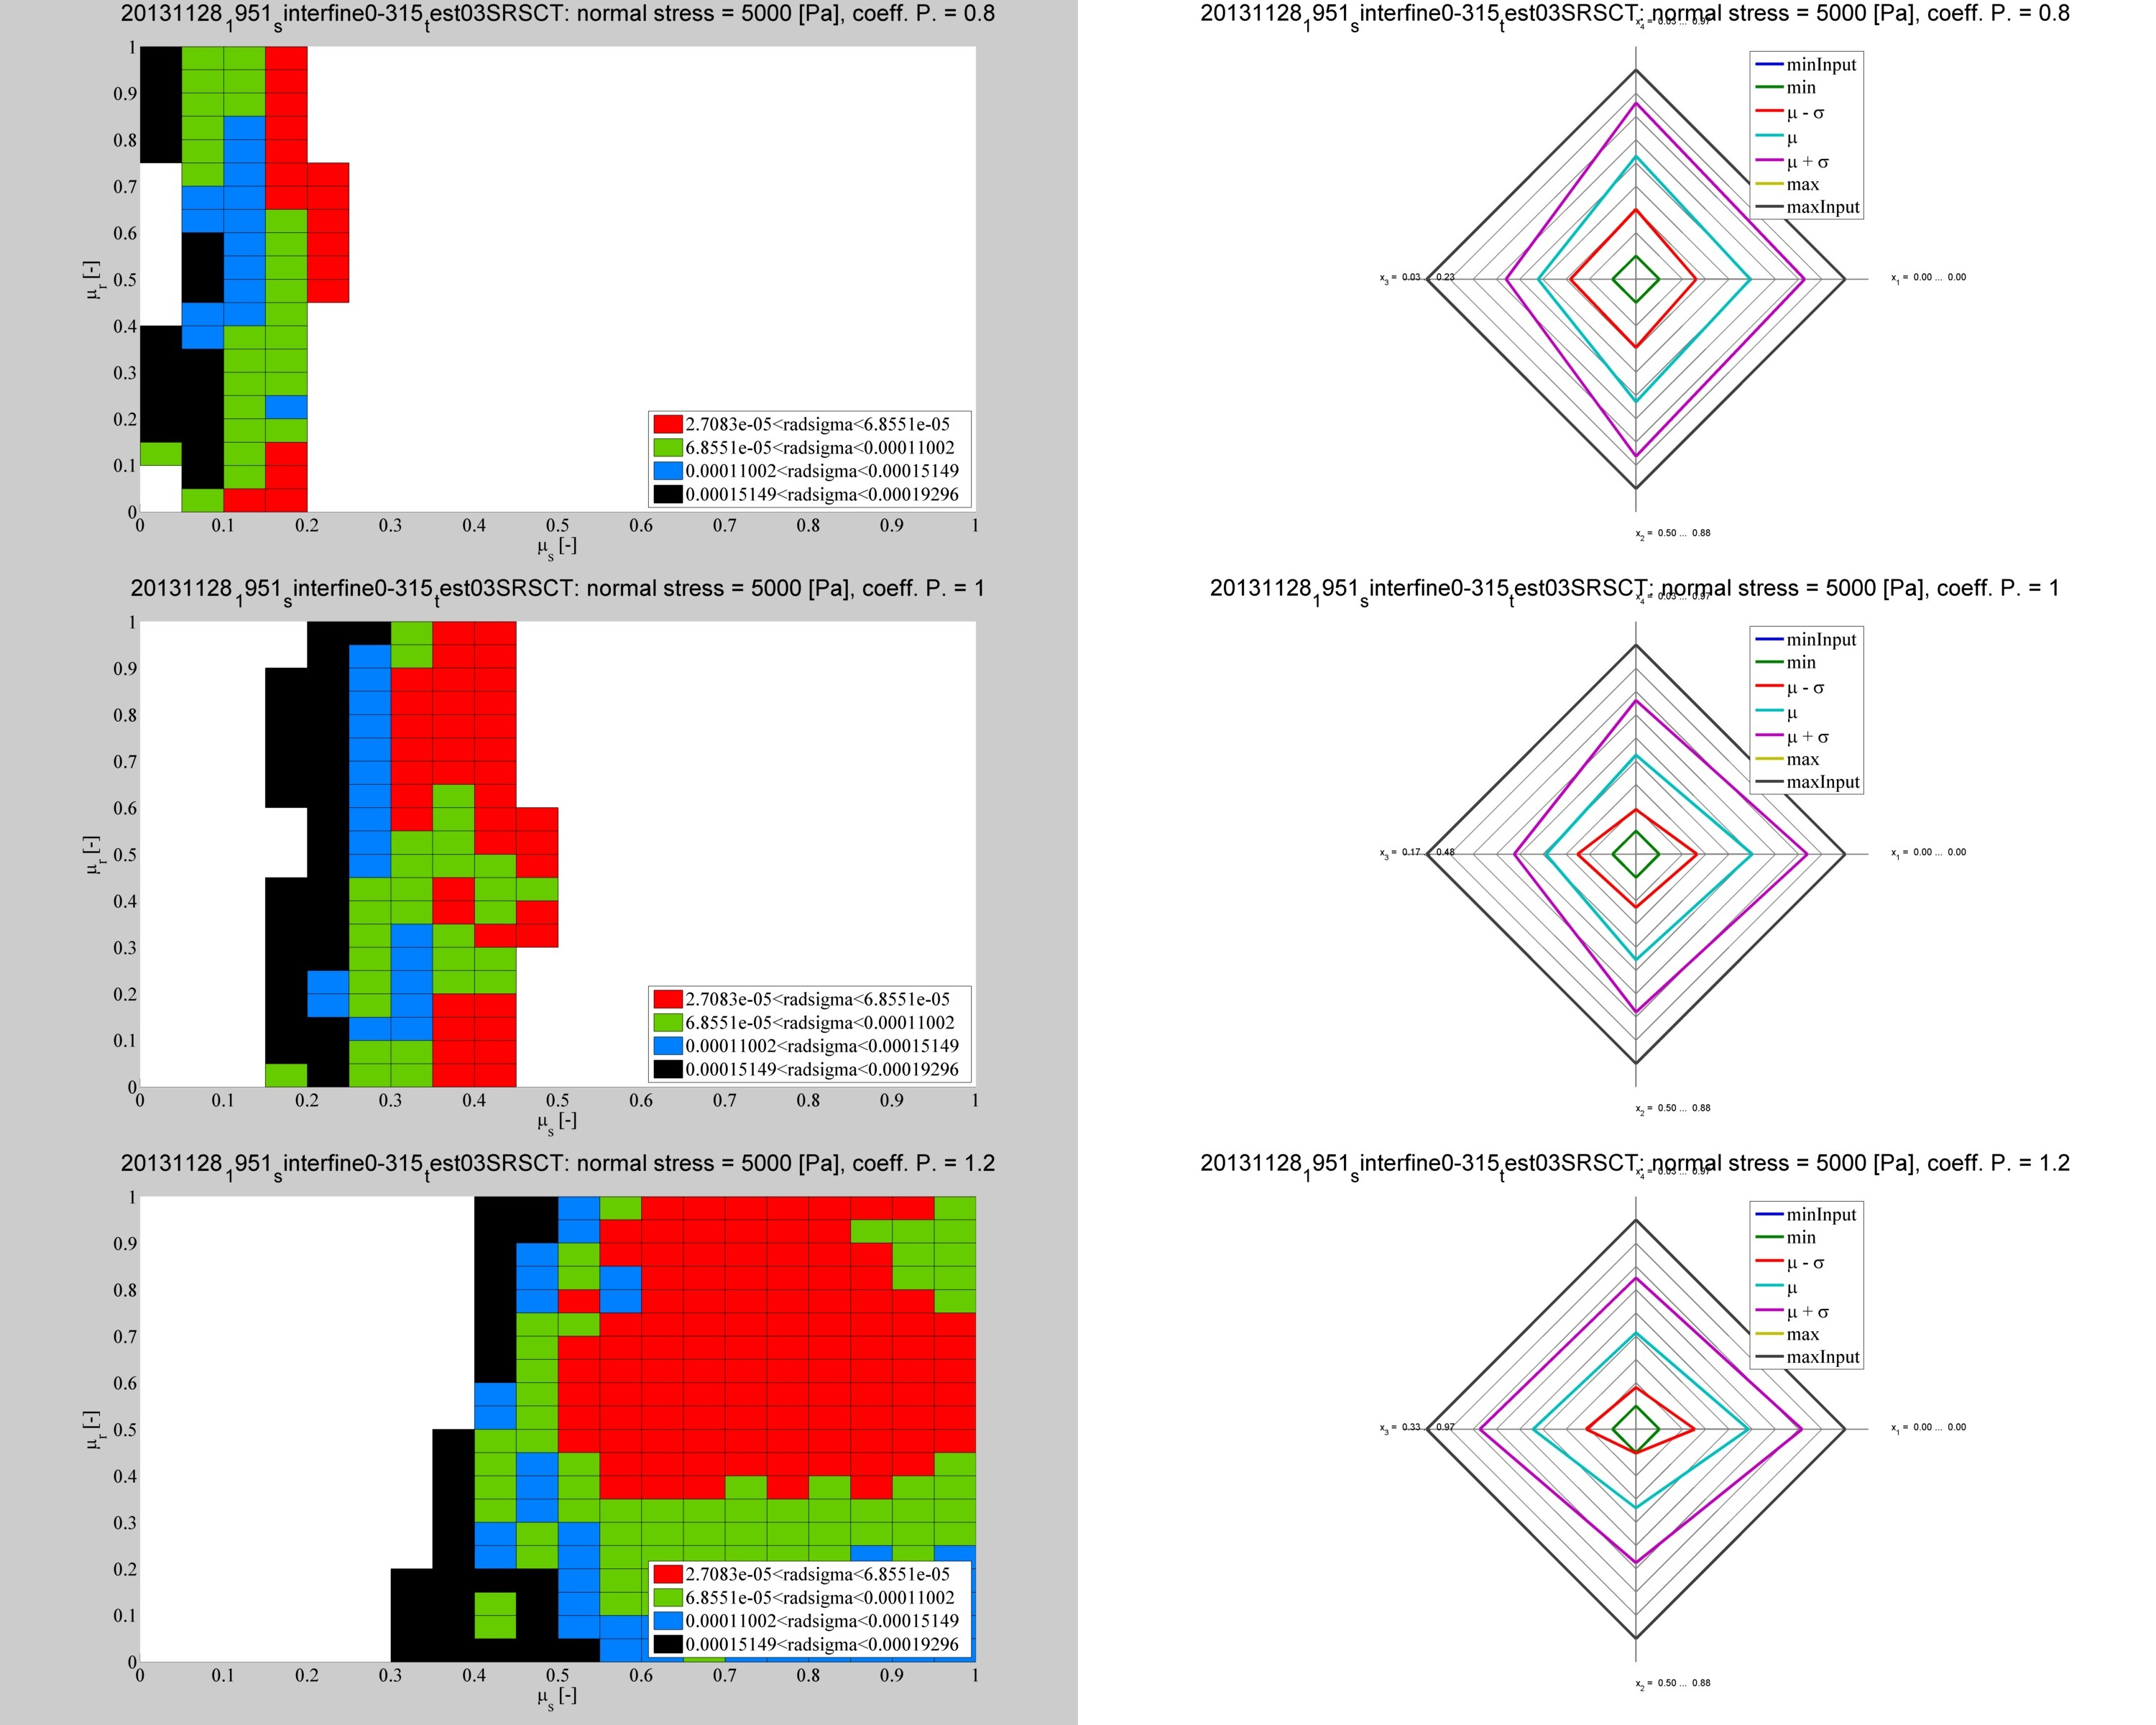
\includegraphics[width=.96\columnwidth]{images/086sinter0315}
\caption[Sinter fine polidispersity evaluation]{Sinter fine polidispersity evaluation.}
\label{fig:086sinter0315}
\end{figure}

Fig. \ref{fig:087sinter31510}\\
\begin{figure}[!htb]
\centering
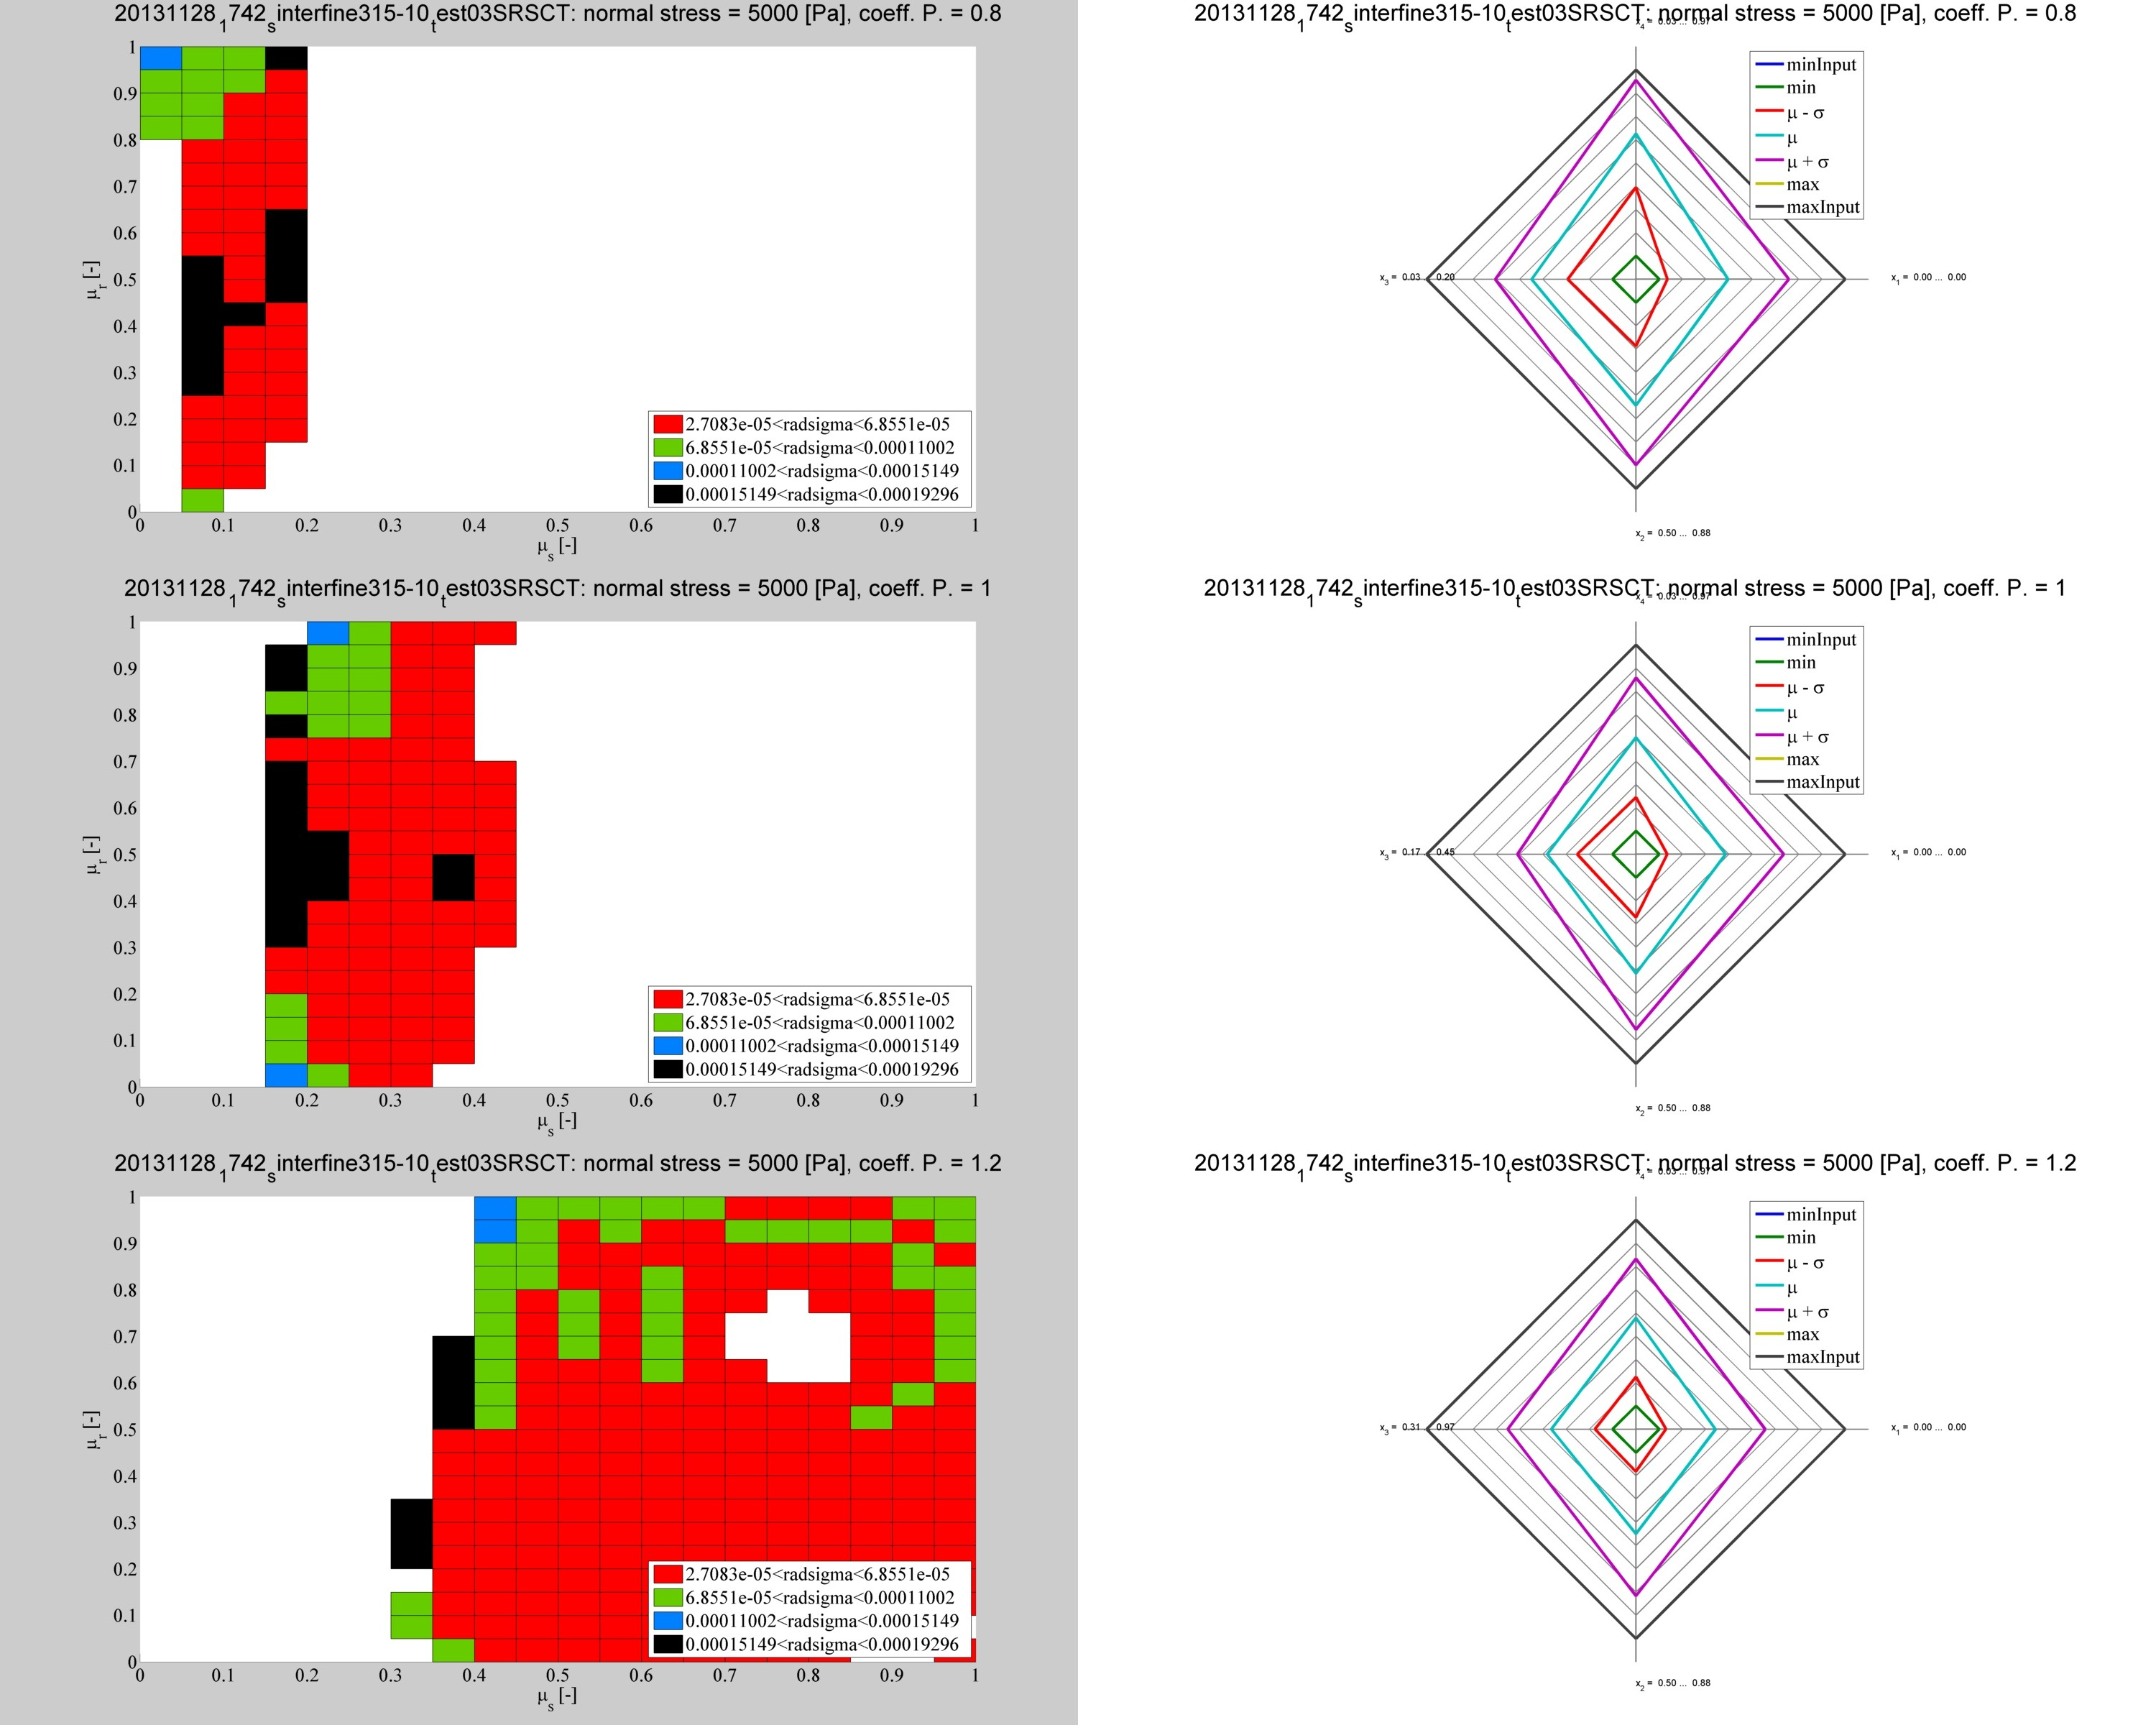
\includegraphics[width=.96\columnwidth]{images/087sinter31510}
\caption[Sinter coarse polydispersity evaluation]{Sinter coarse polydispersity
evaluation.}
\label{fig:087sinter31510}
\end{figure}